\documentclass[10pt]{article}
%\documentclass[11pt,twoside]{book}

\usepackage[utf8]{inputenc}

\usepackage{makeidx}
\usepackage{geometry}%[left=3.5cm,right=3cm,bottom=4cm]%,nohead]
%\geometry{
% a4paper,
% total={210mm,297mm},
% left=2mm,
% right=2mm,
% top=2mm,
% bottom=2mm,
% }
\usepackage{graphicx,graphics}
\usepackage{caption,subcaption}

%\usepackage{color}
%\usepackage{listings} %for algorithms to highlight. 
%%Add code in between \begin{lstlisting} CODE \end{lstlisting}
%\lstset{ %
%    language=MATLAB,                % choose the language of the code
%    basicstyle=\footnotesize,       % the size of the fonts that are used for the code
%    numbers=left,                   % where to put the line-numbers
%    numberstyle=\footnotesize,      % the size of the fonts that are used for the line-numbers
%    stepnumber=1,                   % the step between two line-numbers. If it is 1 each line will be numbered
%    numbersep=5pt,                  % how far the line-numbers are from the code
%    backgroundcolor=\color{white},  % choose the background color. You must add \usepackage{color}
%    showspaces=false,               % show spaces adding particular underscores
%    showstringspaces=false,         % underline spaces within strings
%    showtabs=false,                 % show tabs within strings adding particular underscores
%    frame=single,           % adds a frame around the code
%    tabsize=2,          % sets default tabsize to 2 spaces
%    captionpos=b,           % sets the caption-position to bottom
%    breaklines=true,        % sets automatic line breaking
%    breakatwhitespace=false,    % sets if automatic breaks should only happen at whitespace
%    escapeinside={\%*}{*)}          % if you want to add a comment within your code
%}

\usepackage{amsthm,amsmath,amsfonts,mathtools}

%\DeclareMathAlphabet\mathbfcal{OMS}{cmsy}{b}{n} %mathcal bold

\usepackage{amssymb}

%\usepackage{epsfig} % for postscript graphics files
\usepackage[outdir=./]{epstopdf,epsfig} % eps image attaching
%\usepackage{subfigure}
\usepackage[version=3]{mhchem}
\usepackage{bm}
\usepackage{breqn}
\bibliographystyle{unsrt}
\renewcommand{\baselinestretch}{2}
\usepackage{tikz}
\usetikzlibrary{shapes,shadows,arrows,matrix,positioning}
\usepackage{setspace}
%\onehalfspacing
\singlespacing
\usepackage{wrapfig}
%\usepackage{natbib}
\usepackage{color}
\usepackage{listings}
\usepackage{enumitem}
\setlist{nolistsep}
\raggedbottom %or \usepackage[bottom]{footmisc} %for not having random spacing in pages
\usepackage{pdfpages}
\usepackage{hyperref}
\hypersetup{pdfauthor={Midhun Kathanaruparambil Sukumaran},
    pdftitle={COPASI - a COmplex PAthway SImulator},
	pdfsubject={COPASI},
	pdfkeywords={http://uwaterloo.academia.edu/MidhunKS},
	baseurl={http://uwaterloo.academia.edu/MidhunKS},
	pdfproducer={Midhun Kathanaruparambil Sukumaran},
	pdfcreator={Latex},
	breaklinks=false,
	pdfdisplaydoctitle=true,
	pdfstartpage=1,
	colorlinks=true,
	allcolors=blue,
	%    pdfpagelayout=TwoColumnLeft ,
	%    pdfpagemode=FullScreen,
	%pdfnumcopies=2,
	%    pdfpagetransition=Wipe,
	%    pdftoolbar=false,
	%hidelinks
}
\usepackage{hypcap}
%\usepackage{titling}

\newcounter{example}[section]
\newenvironment{example}[1][]{\refstepcounter{example}\par\medskip
	\textbf{Step~\theexample. #1} \rmfamily}{\medskip}


\title{\LARGE COPASI - a COmplex PAthway SImulator}
\author{Midhun Kathanaruparambil Sukumaran and Brian P Ingalls\\
	2016 Connaught Summer Institute for Synthetic Biology\\
	University of Toronto}% <-this % stops a space
%%\thanks{*This work was supported by organization}% <-this % stops a space
%%\thanks{$^{1}$Albert Author is with Faculty of Electrical Engineering, Mathematics and Computer Science,
%% University of Twente, 7500 AE Enschede, The Netherlands
%% {\tt\small albert.author@papercept.net}}%
%%\thanks{$^{2}$Bernard D. Researcheris with the Department of Electrical Engineering, Wright State University,
%% Dayton, OH 45435, USA
%% {\tt\small b.d.researcher@ieee.org}}%
%}
\date{June 6-10, 2016}
%\title{\ttitle} % Defines the thesis title - don't touch this
\newtheorem{thm}{Theorem}%[chapter]
\newtheorem{prop}{Proposition}[thm]
\newtheorem{lem}{Lemma}[thm]
\newtheorem{cor}{Corollary}[thm]

\theoremstyle{definition}
\newtheorem{mydef}{Definition}[thm]
\newtheorem{ex}{Example}[thm]

\theoremstyle{remark}
\newtheorem{remark}[thm]{Remark}

\begin{document}
	\maketitle    
	\section*{Prerequisites}
	\begin{enumerate}
		\item Install COPASI : \href{http://copasi.org/Download/}{http://copasi.org/Download/}
		\item Download COPASI models from the summer school  \href{https://www.dropbox.com/sh/b2ue0vo0ujyiroc/AADXPVi5s3kFIeVIrPtR29Yaa?dl=0}{dropbox folder}
	\end{enumerate}
	
	\section*{Additional Information}
	\begin{enumerate}
		\item Documentation: \href{http://copasi.org/Support/User_Manual/}{http://copasi.org/Support/User\_Manual/}
		\item Video Tutorial: \href{http://copasi.org/Support/Video_Tutorials/}{http://copasi.org/Support/Video\_Tutorials/}
	\end{enumerate}
	\section{Interface-Figure~\ref{1png}}
	\begin{figure}[h]
		\centering
		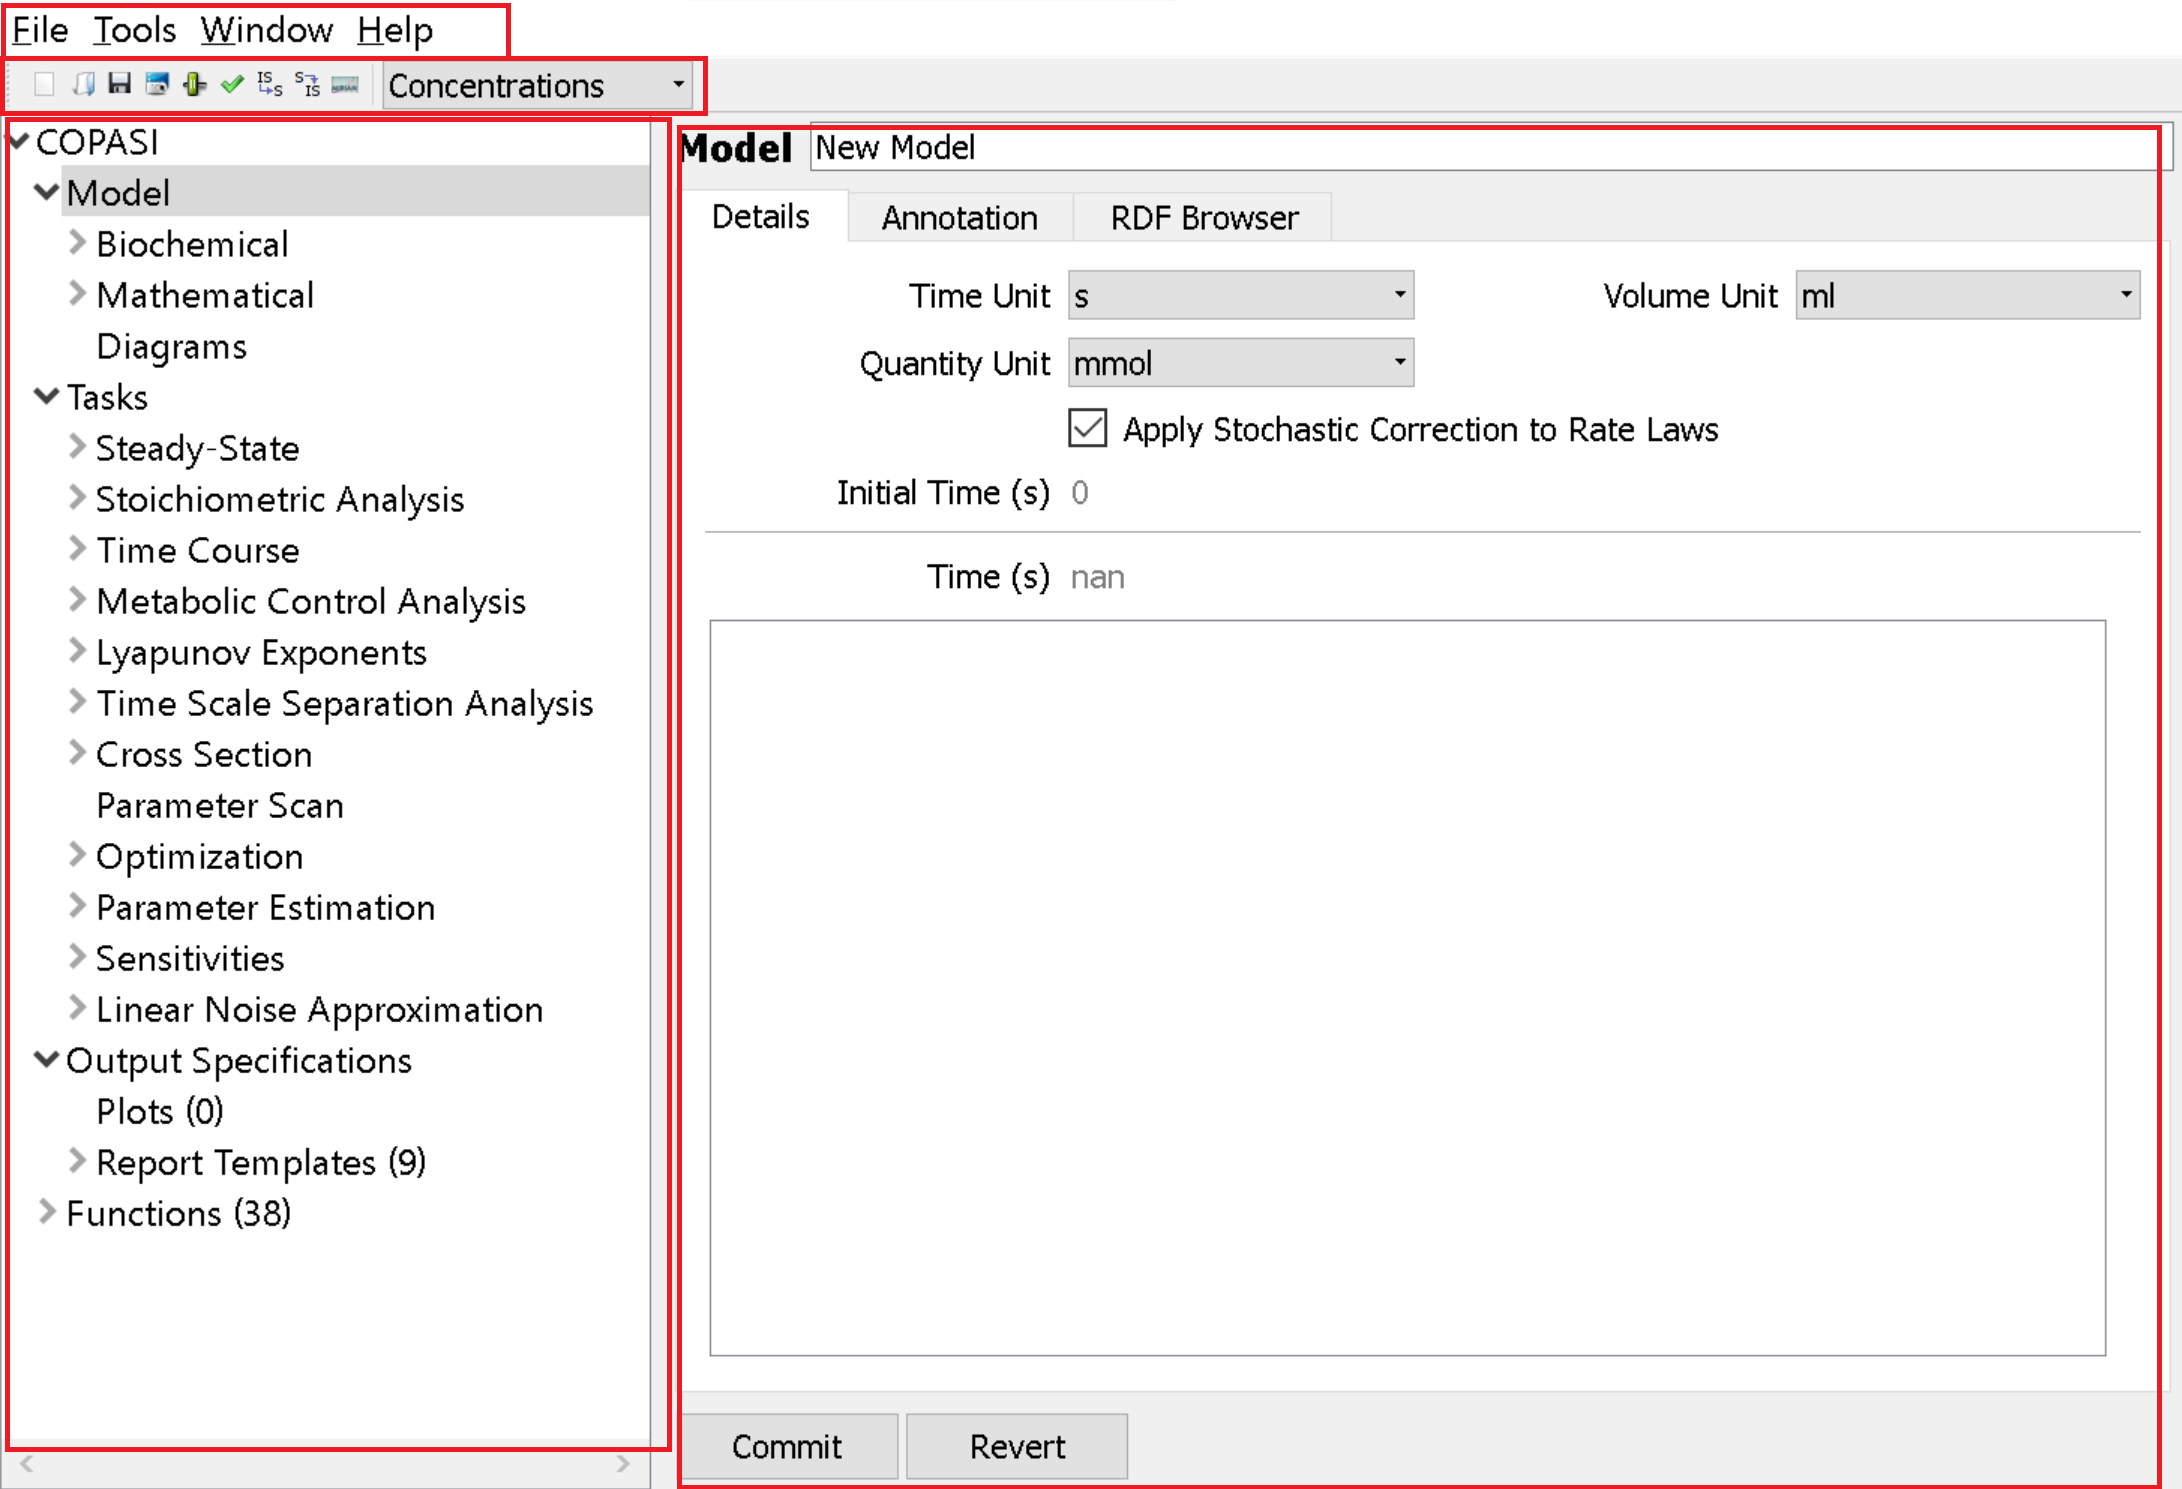
\includegraphics[height=10cm]{Images/1.png}
		\caption{Interface}
		\label{1png}
	\end{figure}
	COPASI's interface split into four parts including the major workspace which is divided into two parts (\textbf{Object tree} and \textbf{Editor}).
	
	\subsection{Menu Bar}
	Position : Top row\\
	Components: \textbf{File}, \textbf{Tools}, \textbf{Window}, \textbf{Help}
	
	\subsection{Tool Bar}
	Position: Row below \textbf{Menu bar}\\
	Components: \textbf{Open}, \textbf{Save}, \textbf{Print}, etc.
	
	\subsection{Object Tree}
	Position: Left column below \textbf{Tool bar}\\
	Components: Main routines such as \textbf{Model}, \textbf{Tasks}, \textbf{Output specifications}, and \textbf{Functions}. Each of these has subroutines such as \textbf{Biochemical}, \textbf{Mathematical}, etc.
	
	\subsection{Editor}
	Position : Right column below \textbf{Tool bar}\\
	Components: Varies according to the chosen routine in the \textbf{Object tree}
	
	\section{Model Creation}
	Basic requirements to generate a COPASI model is the knowledge of the biochemical network, rate laws, and possible compartments. Parameters such as initial concentration and rate constants can be identified through parameter estimation methods using experimental data. Let's start with a simple linear chemical system
	\[\ce{A <=>[10][20] B <=>[15][50] C}\]
	Species: A, B, and C.\\
	Rate constants: 10/s, 20/s, 15/s, and 50/s.\\
	Initial molecular population: A= 0.1$\mu$mol, B=1$\mu$mol, and C =$0$.\\
	Compartment Volume:$10 fl$.\\
	\begin{enumerate}\def\makelabel{\textbf{Step}~}
		\item Open \textbf{Copasi UI}
		\item Expand \textbf{COPASI} in the \textbf{Object tree}
		\item Expand \textbf{Model}\\
		\item {\Large\textbf{Model initial setup}}-Figure~\ref{2png}\\
		The first step is to define the model name, units of different types of parameters, and a little description about the model.
		\begin{figure}[!htb]
			\centering
			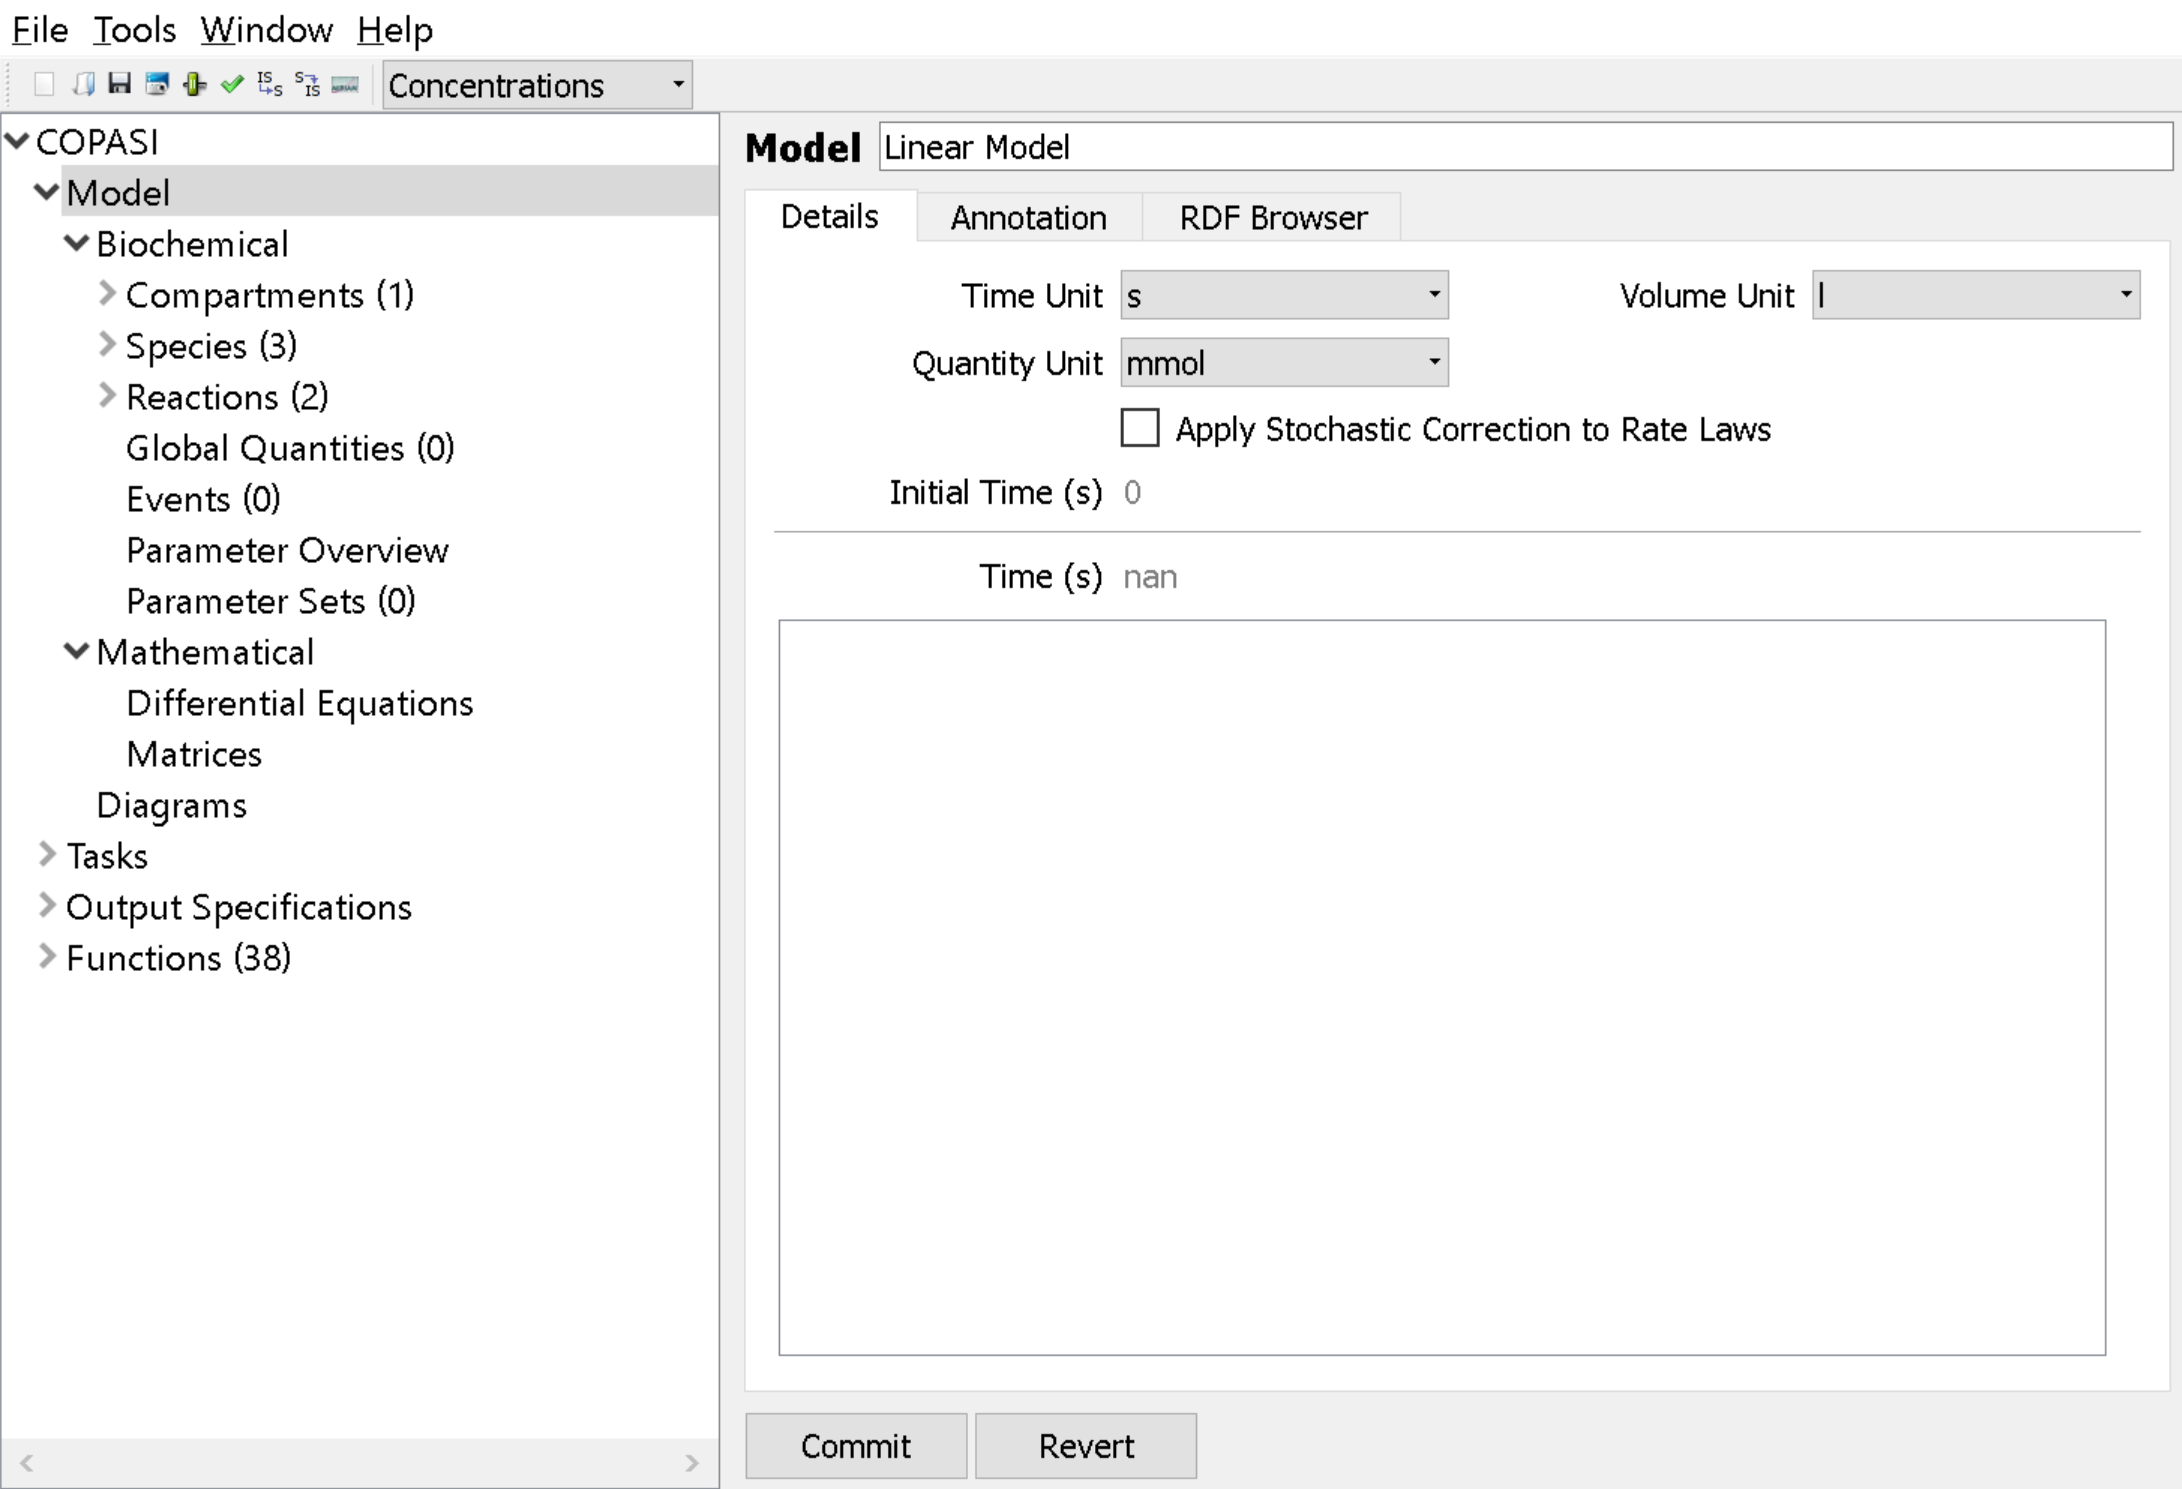
\includegraphics[height=10cm]{Images/2.png}    
			\caption{model initial setup}
			\label{2png}
		\end{figure}
		\begin{enumerate}
			\item Select \textbf{Biochemical}
			\item Type a model name (\textbf{Linear Model}) in the cell next to \textbf{model} in the editor pane.
			\item In the \textbf{Details} tab, choose units for time (\textbf{s}), volume (\textbf{l}), and quantity (\textbf{mol}).
			\item (optional) Check \textbf{Apply Stochastic Correction to Rate Laws}.
			\item (optional) Type a description of the model.\\
		\end{enumerate}
		\item {\Large\textbf{Reactions setup}}-Figure~\ref{3png}\\
		The second step is to define the biochemical network by entering reactions of the system. This step will define species, reaction rates, and compartments in COPASI. Therefore, we can skip two routines (\textbf{Compartment} and \textbf{Species}) which are generated automatically.
		
		\begin{figure}[!htb]
			\centering
			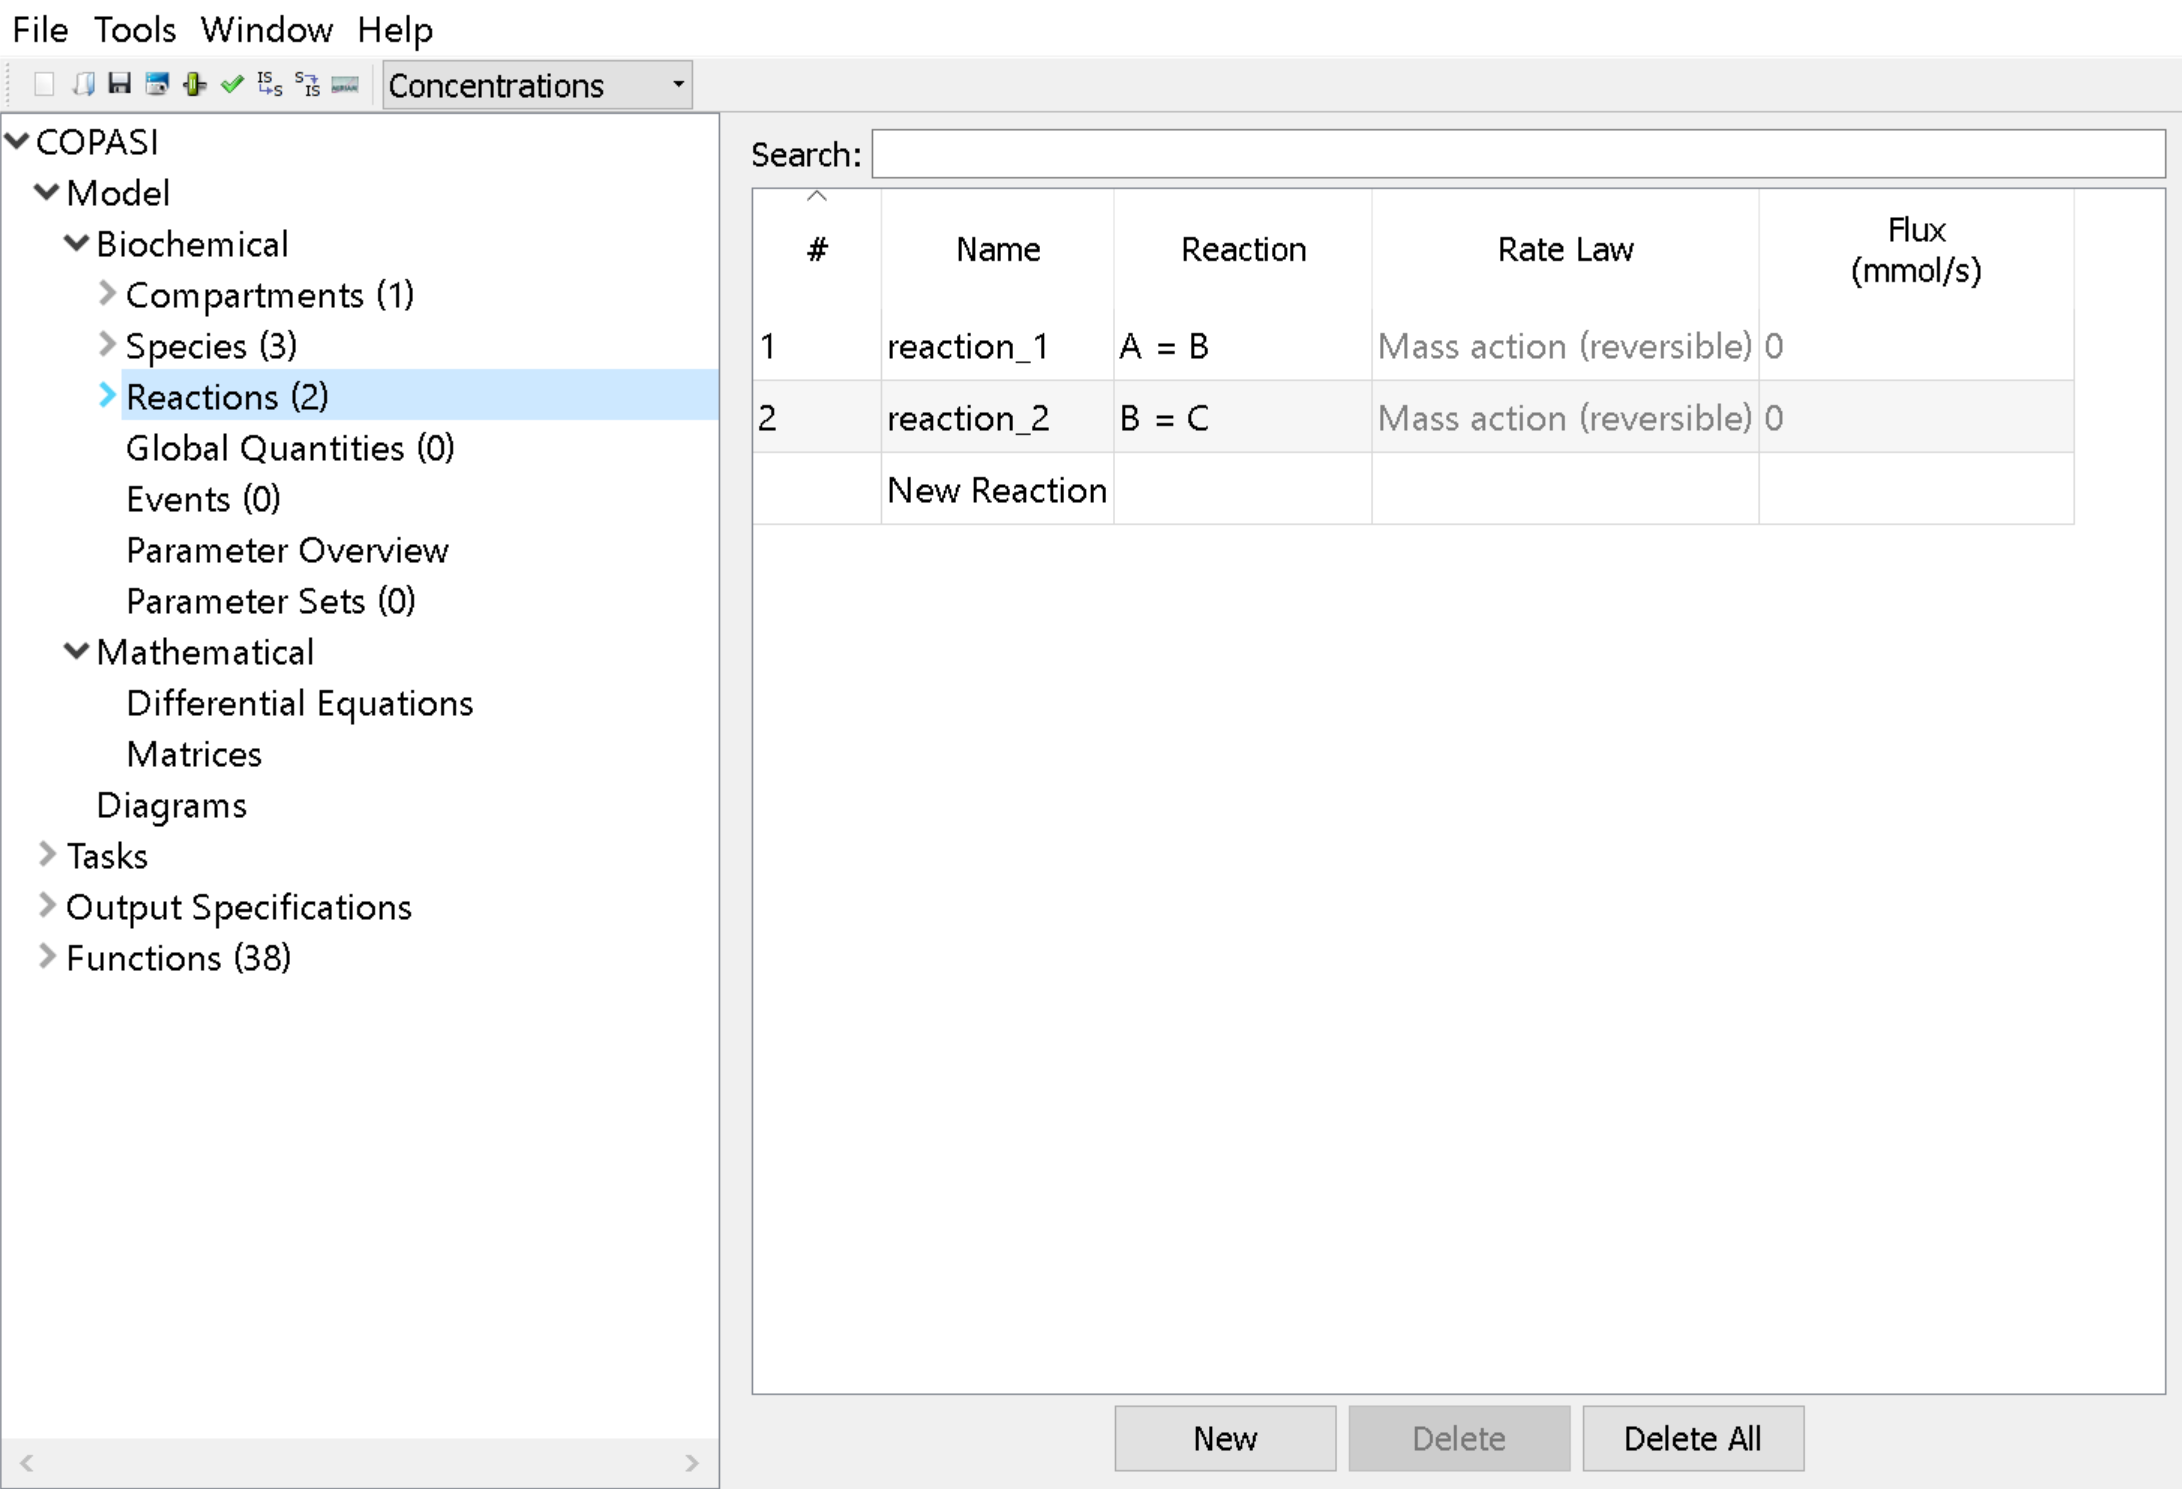
\includegraphics[height=5cm]{Images/3a.png}
			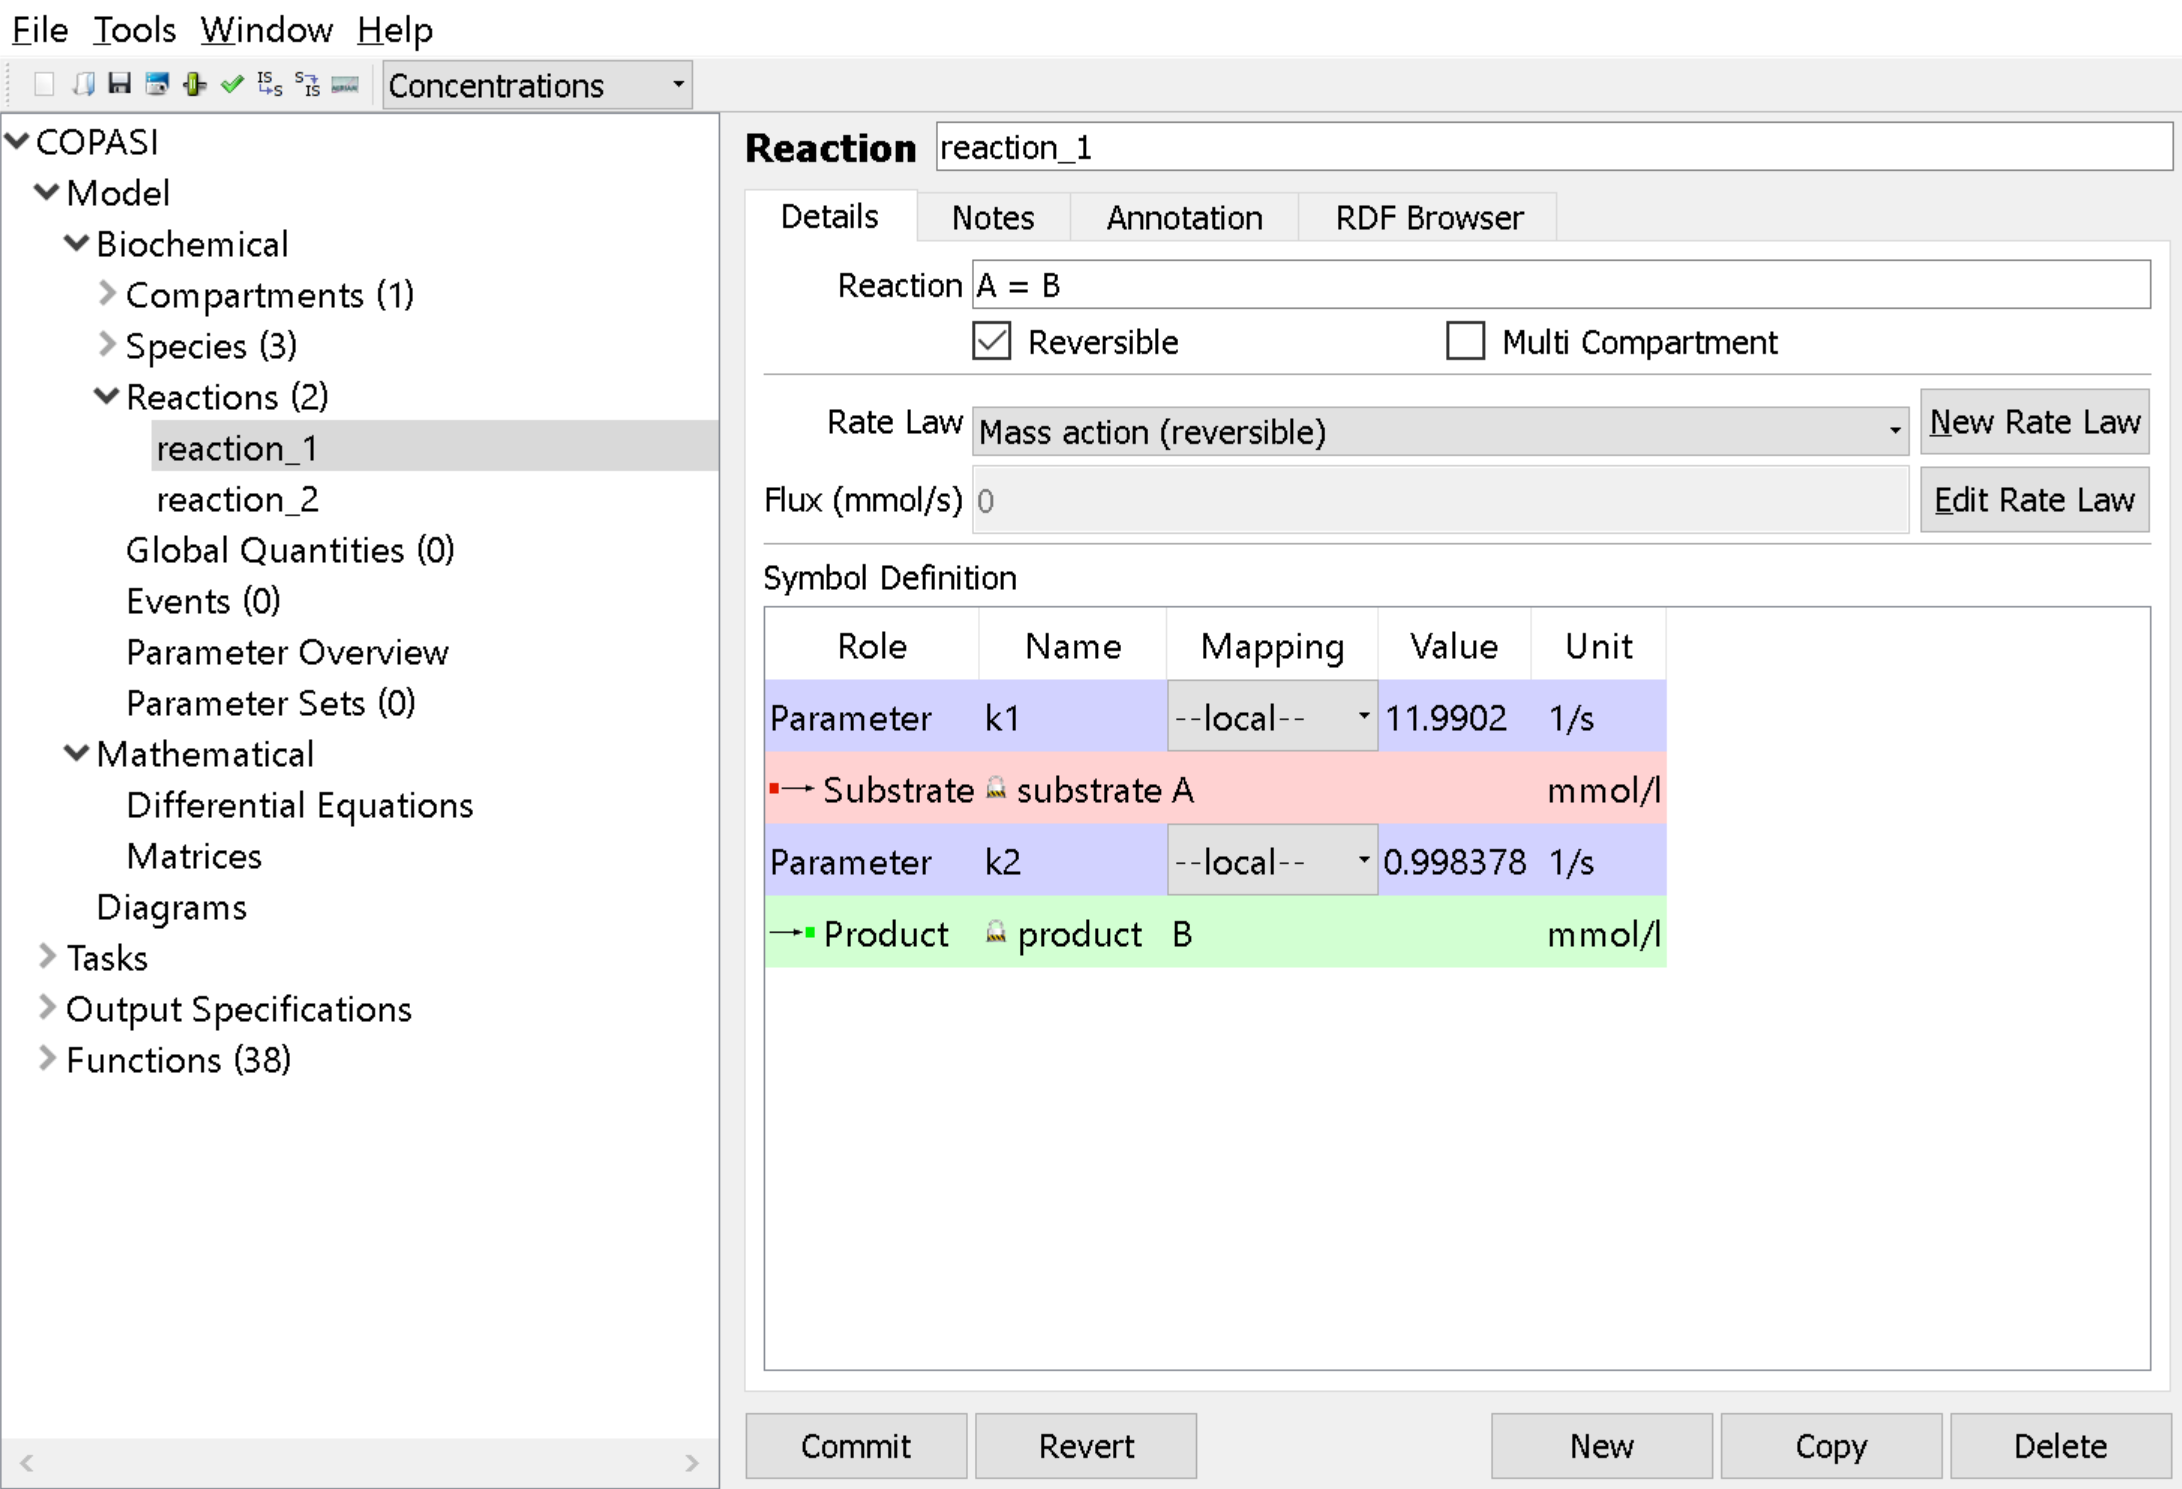
\includegraphics[height=5cm]{Images/3b.png}
			%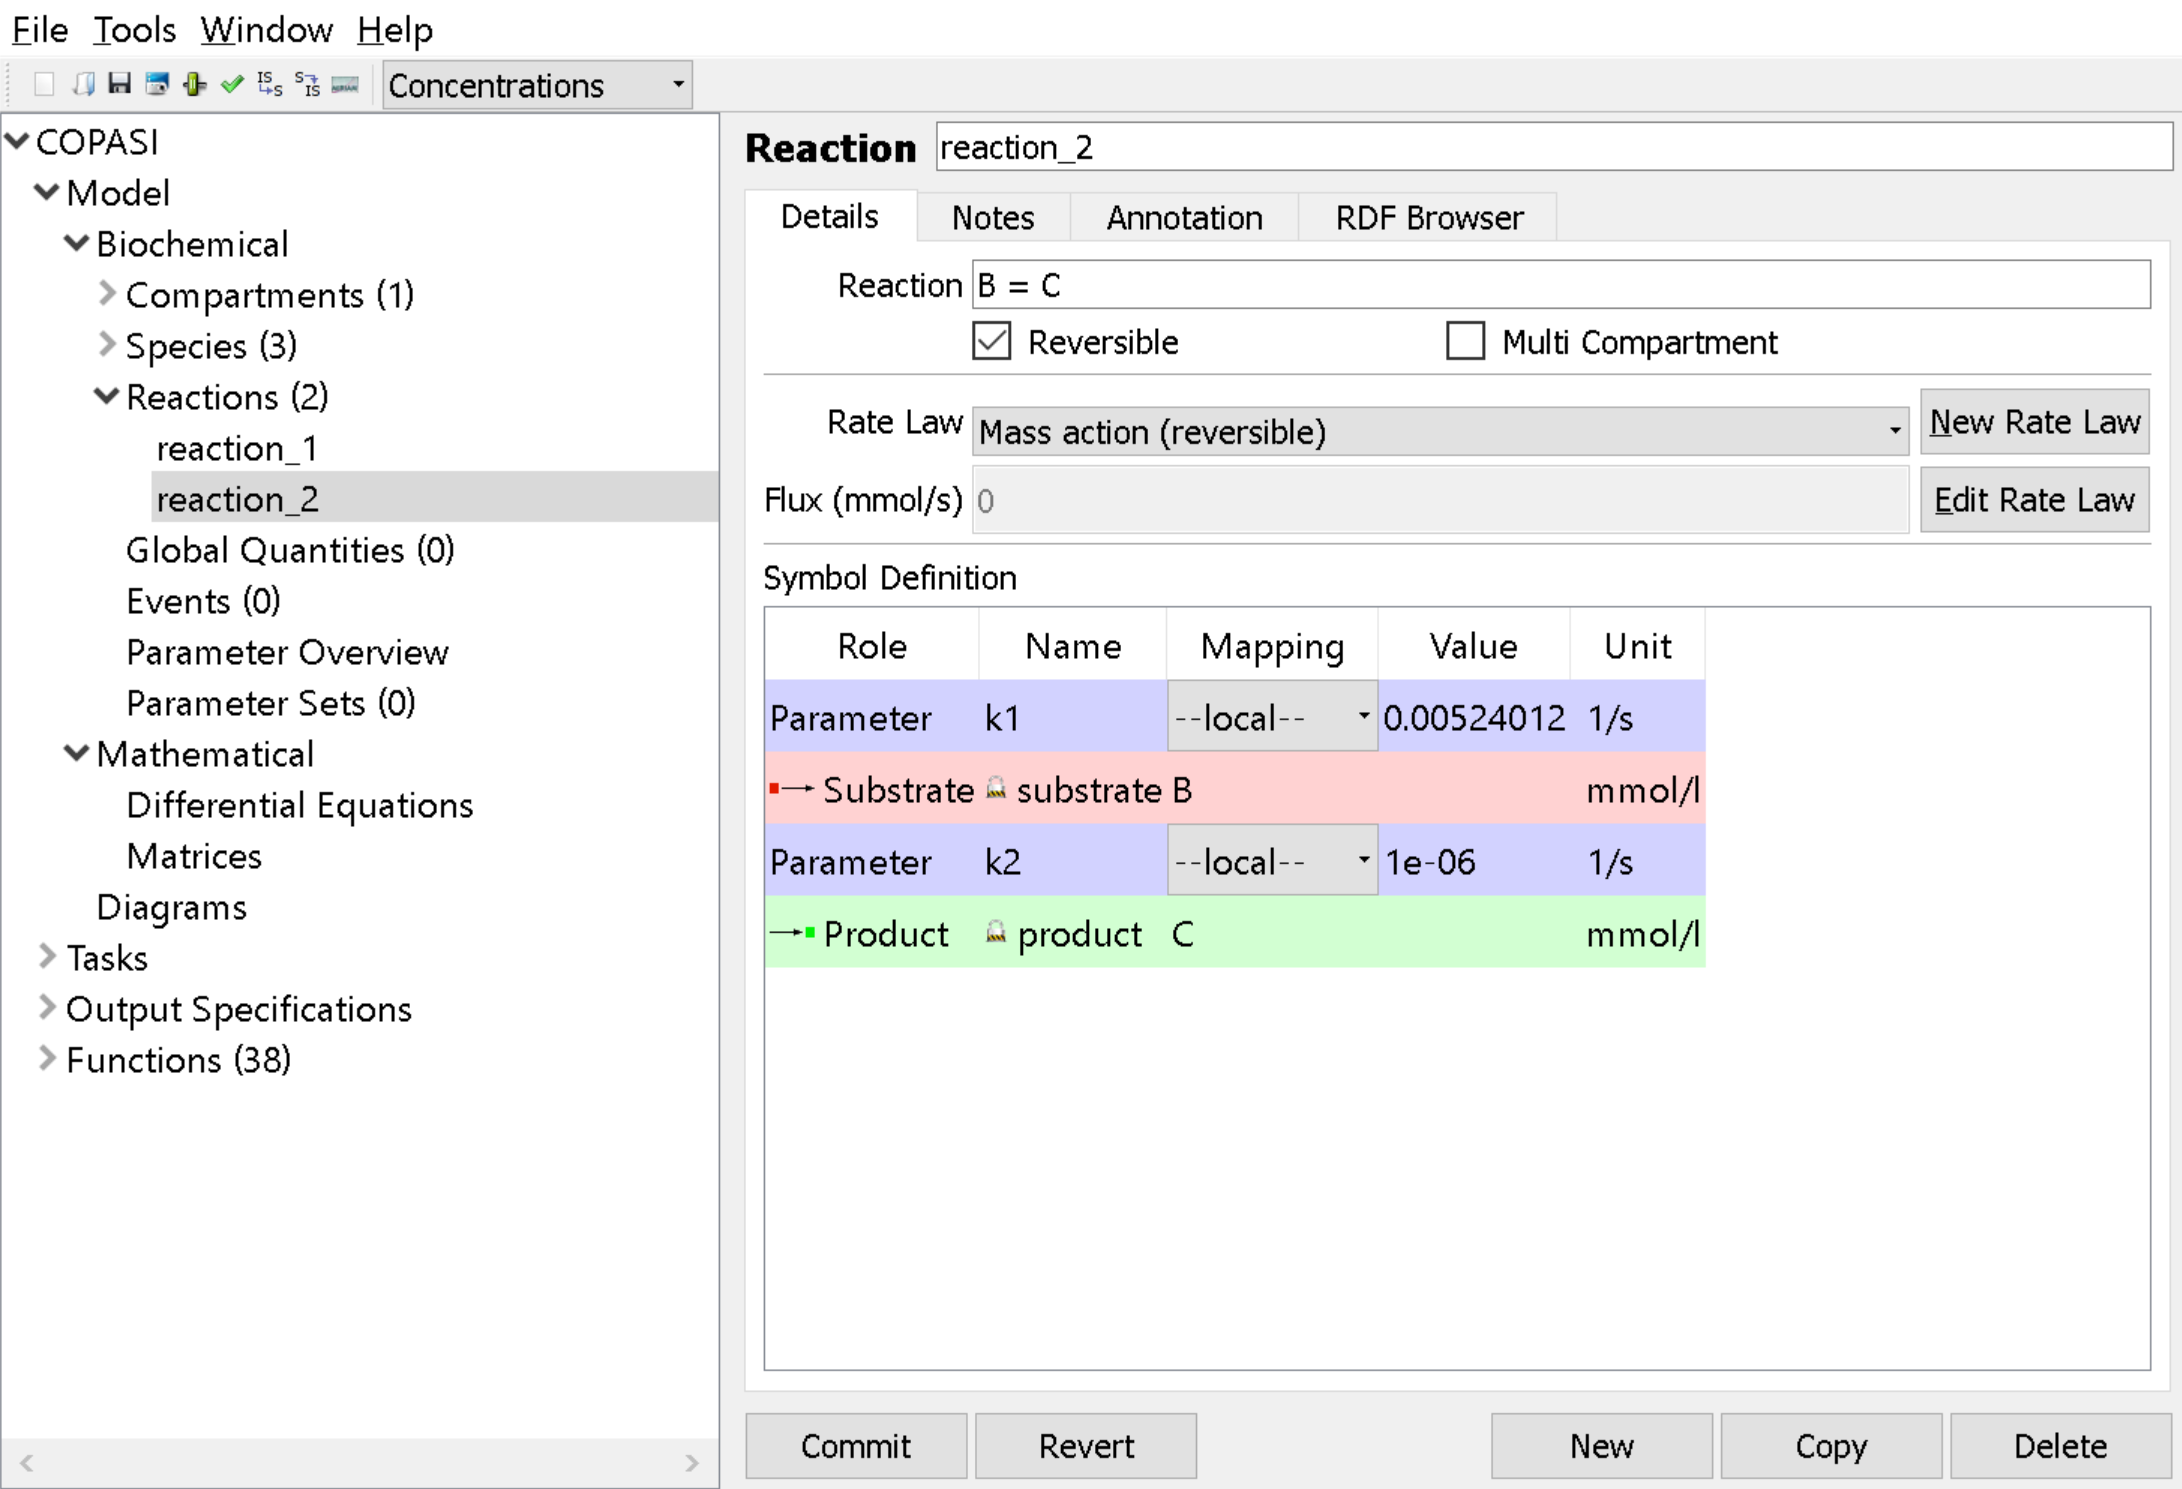
\includegraphics[height=5cm]{Images/3c.png}    
			\caption{Reaction setup}
			\label{3png}
		\end{figure}
		\begin{enumerate} 
			\item Select \textbf{Reactions} in the \textbf{Object tree}.
			\item Select \textbf{New} two times in the \textbf{Editor} pane to create two reactions (Note: see newly created reactions in the \textbf{Object tree} under \textbf{Reactions} -  expand \textbf{Reactions} if needed).
			\item Select \textbf{reactions\_1} under \textbf{Reactions} in the \textbf{Object tree}.
			\item (optional) In the \textbf{Editor} pane, choose a name (cell next to \textbf{Reaction}) for \textbf{reaction\_1}.
			\item In the \textbf{Details} tab, enter first reversible reaction $\ce{A <=>[10][20] B}$ as \textbf{A = B}. (Note the space before and after equal sign) Equal sign represents a reversible reaction and $-$$>$ represents an irreversible reaction.
			\item Choose the \textbf{Rate law} for the reaction. In default, rate law is \textbf{Mass action}. However, we can choose the one we needed. For now, we keep the rate law as \textbf{Mass action (reversible)}. 
			\item In \textbf{Symbol definition} box, under \textbf{Value} column, change the rate constant values to \textbf{10} and \textbf{20}.
			\item Repeat the steps e-g for \textbf{reaction\_2}.\\
		\end{enumerate}
		\item {\Large\textbf{Compartments setup}}-Figure~\ref{4png} \\
		\begin{figure}[!htb]
			\centering
			%     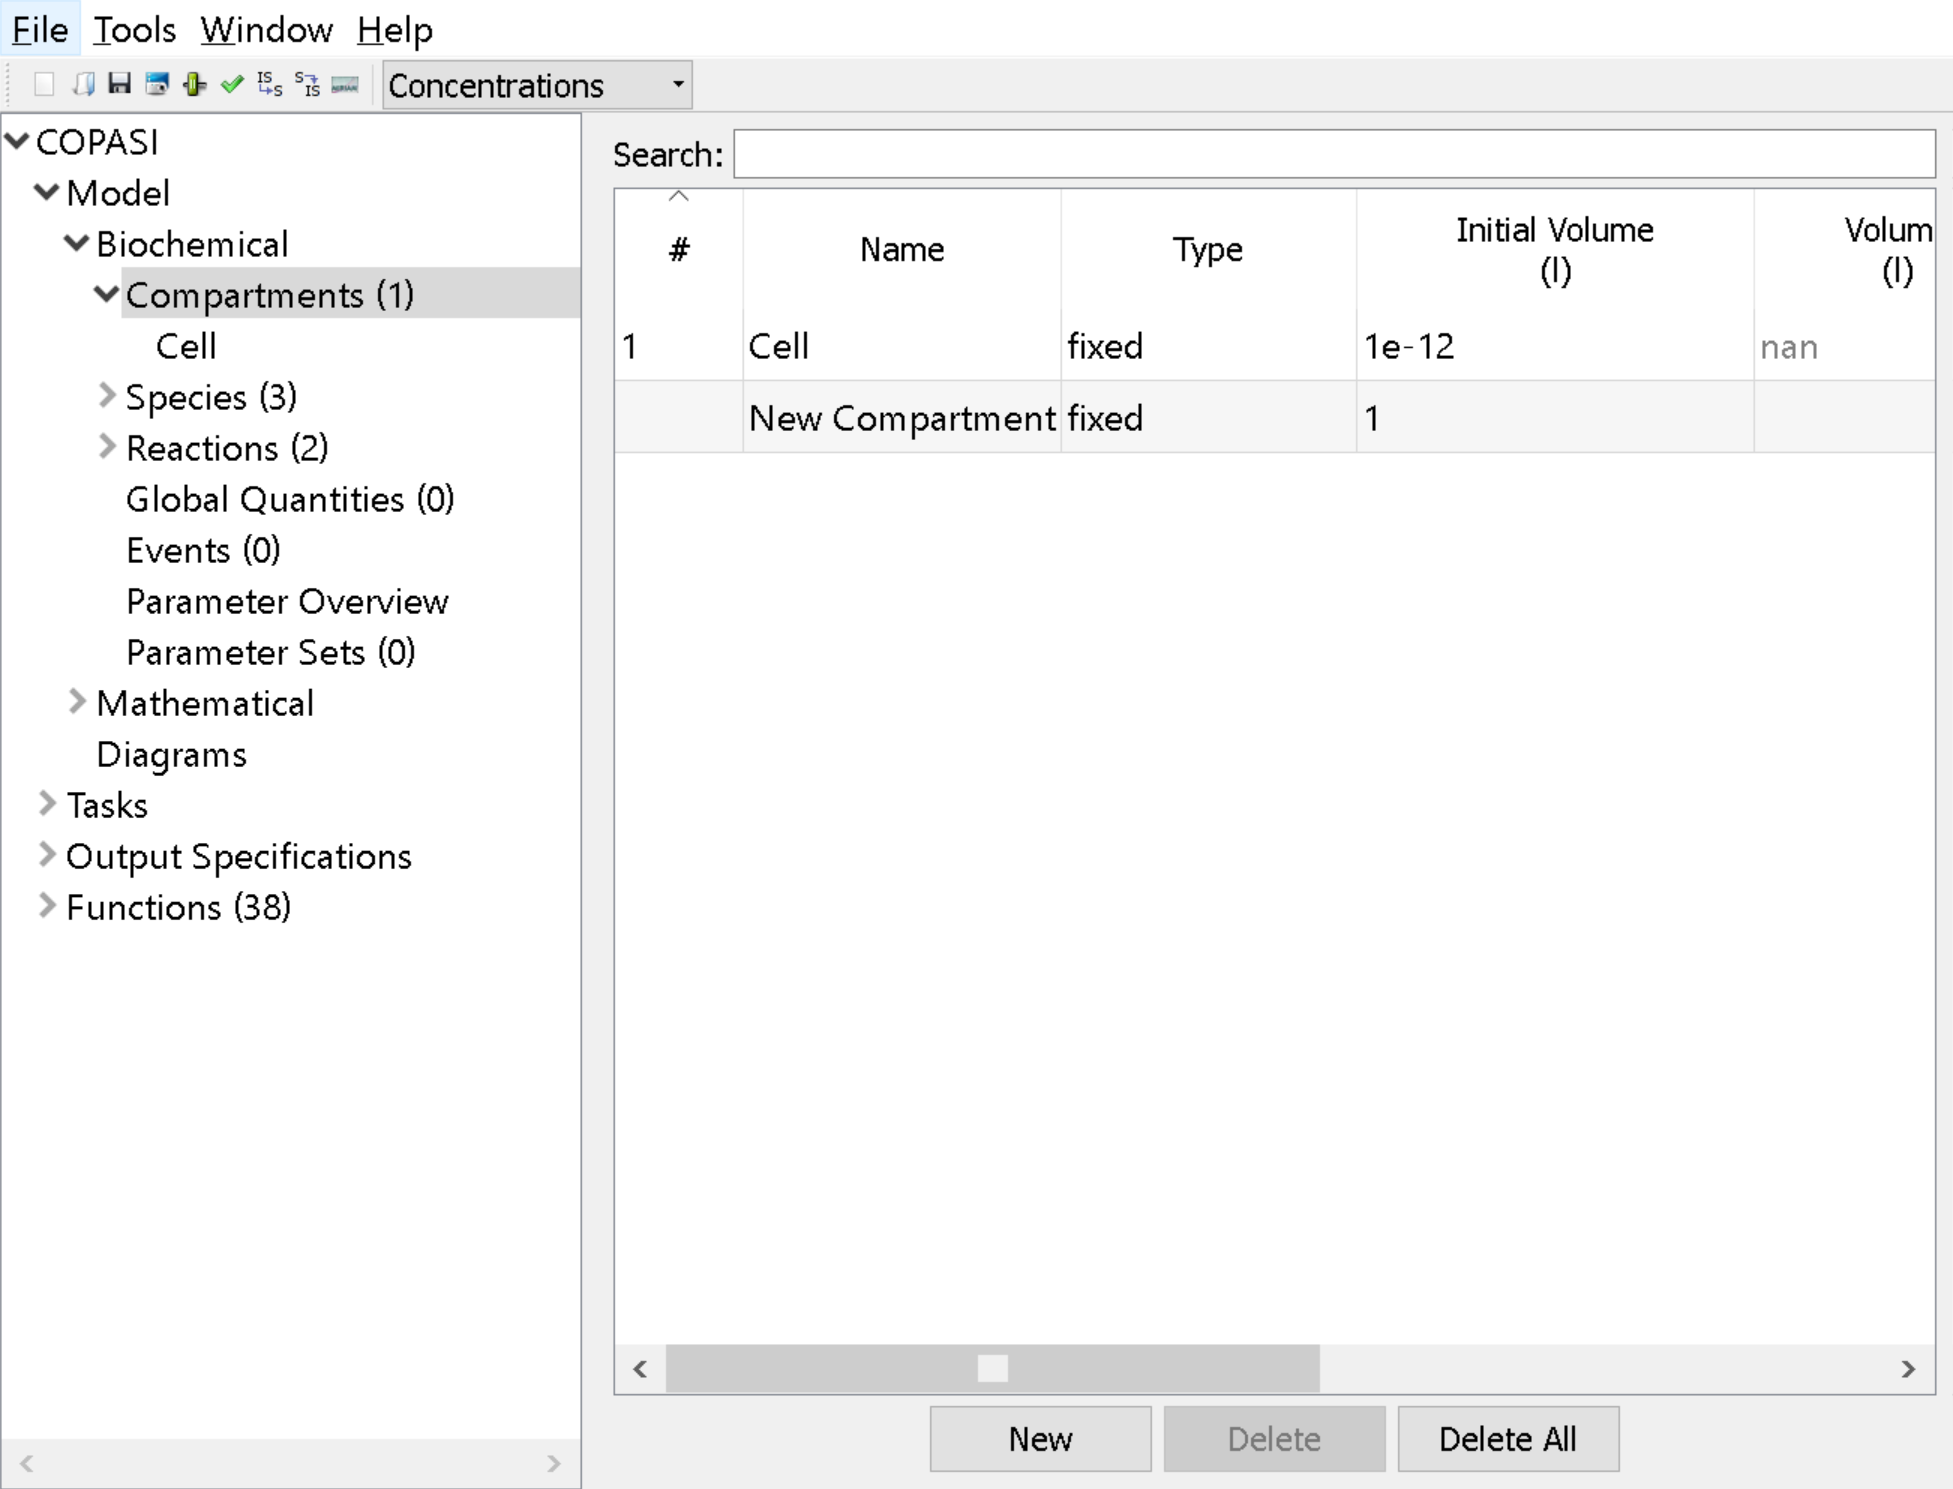
\includegraphics[height=5cm]{Images/4a.png}
			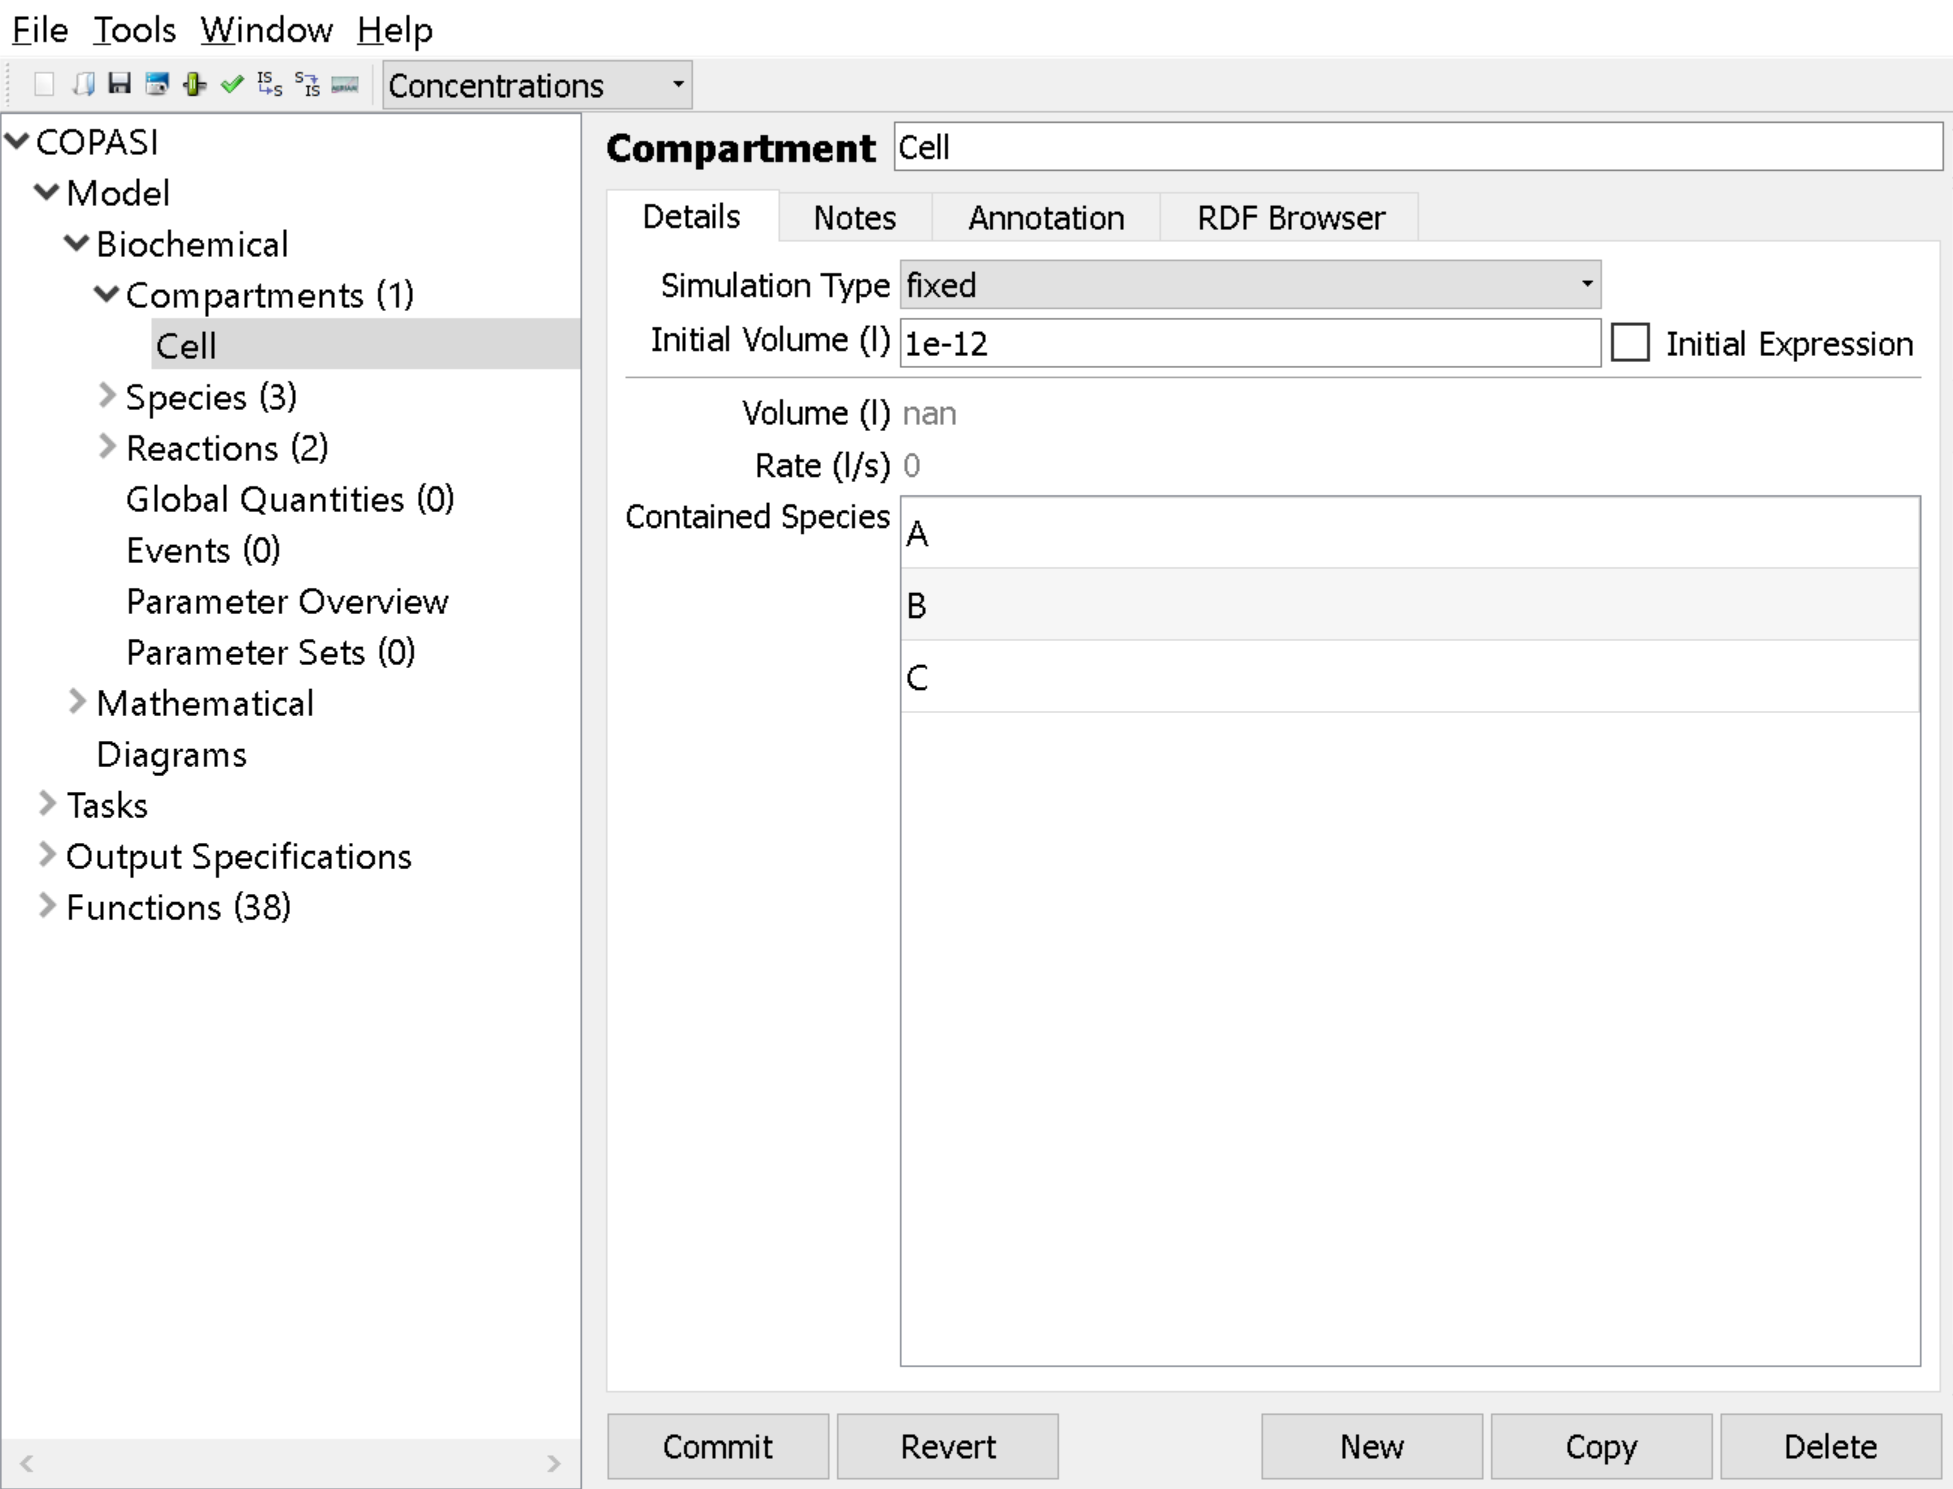
\includegraphics[height=10cm]{Images/4b.png}
			\caption{Compartment setup}
			\label{4png}
		\end{figure}
In COPASI, all reactions are happening in compartments. For e.g. reactions occurring in different organelles of a cell. Even though compartments are generated after reaction setup, we need to define the volume and type of variability of each compartment's volume. 
		\begin{enumerate} 
			\item In \textbf{Object tree}, under \textbf{Compartments}, select \textbf{compartment}.
			\item (optional) In the \textbf{Editor} pane (next to \textbf{Compartment}), Change compartment name (\textbf{Cell}).
			\item Under \textbf{Details} tab, enter \textbf{initial volume} as $10e-15$(represents $10^{-15}$).\\
		\end{enumerate}
		\item {\Large\textbf{Species setup}}-Figure~\ref{5png}\\
		\begin{figure}[!htb]
			\centering
			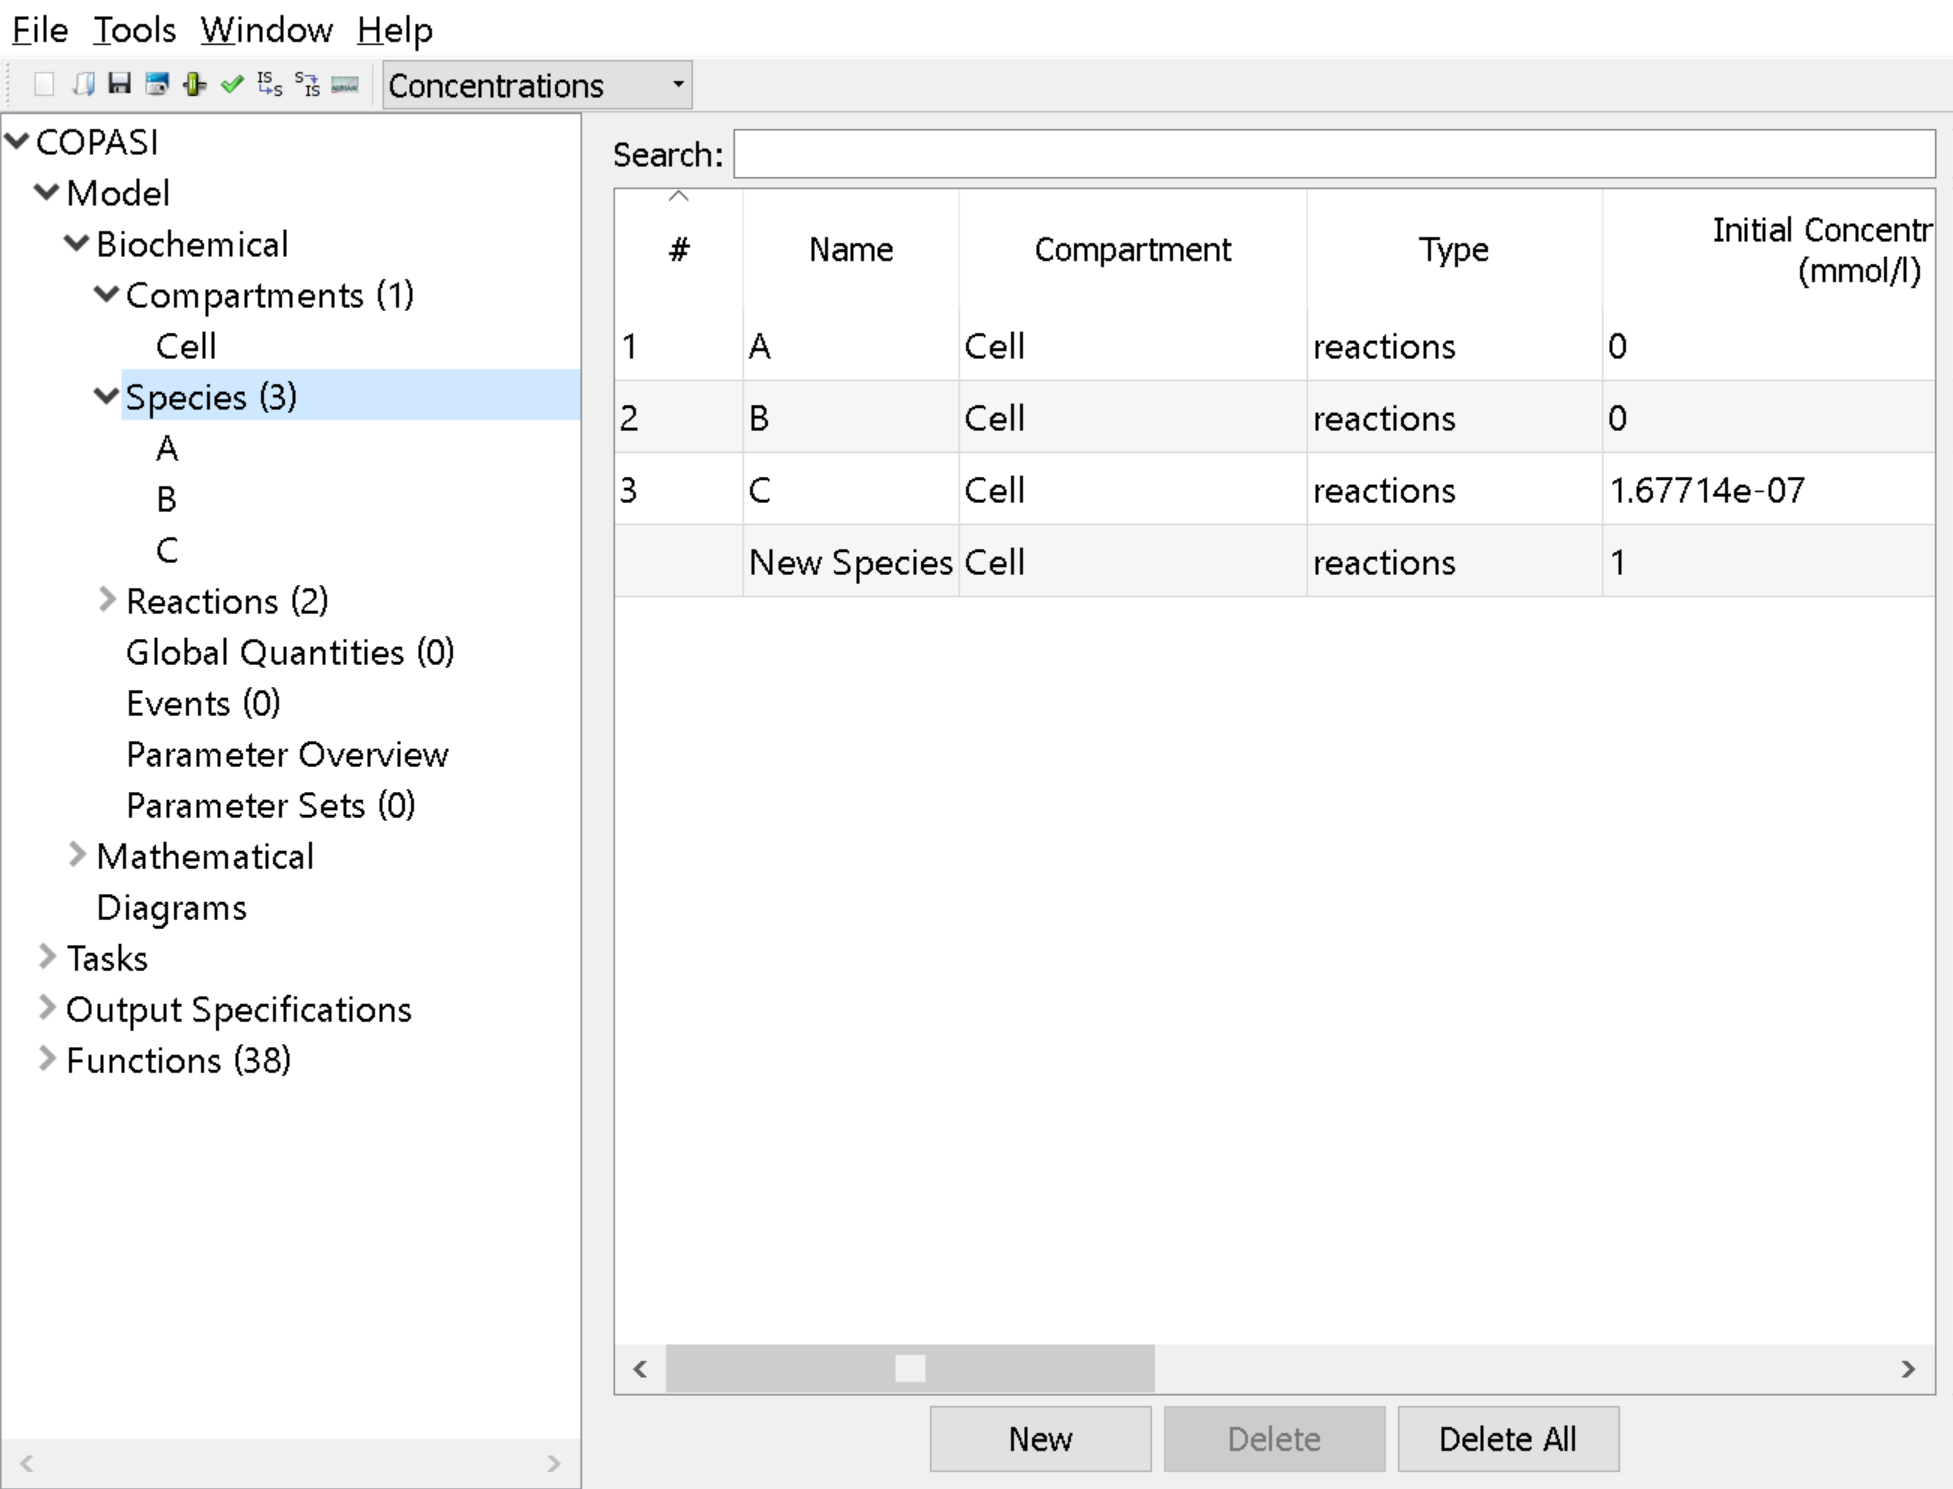
\includegraphics[height=5cm]{Images/5a.png}
			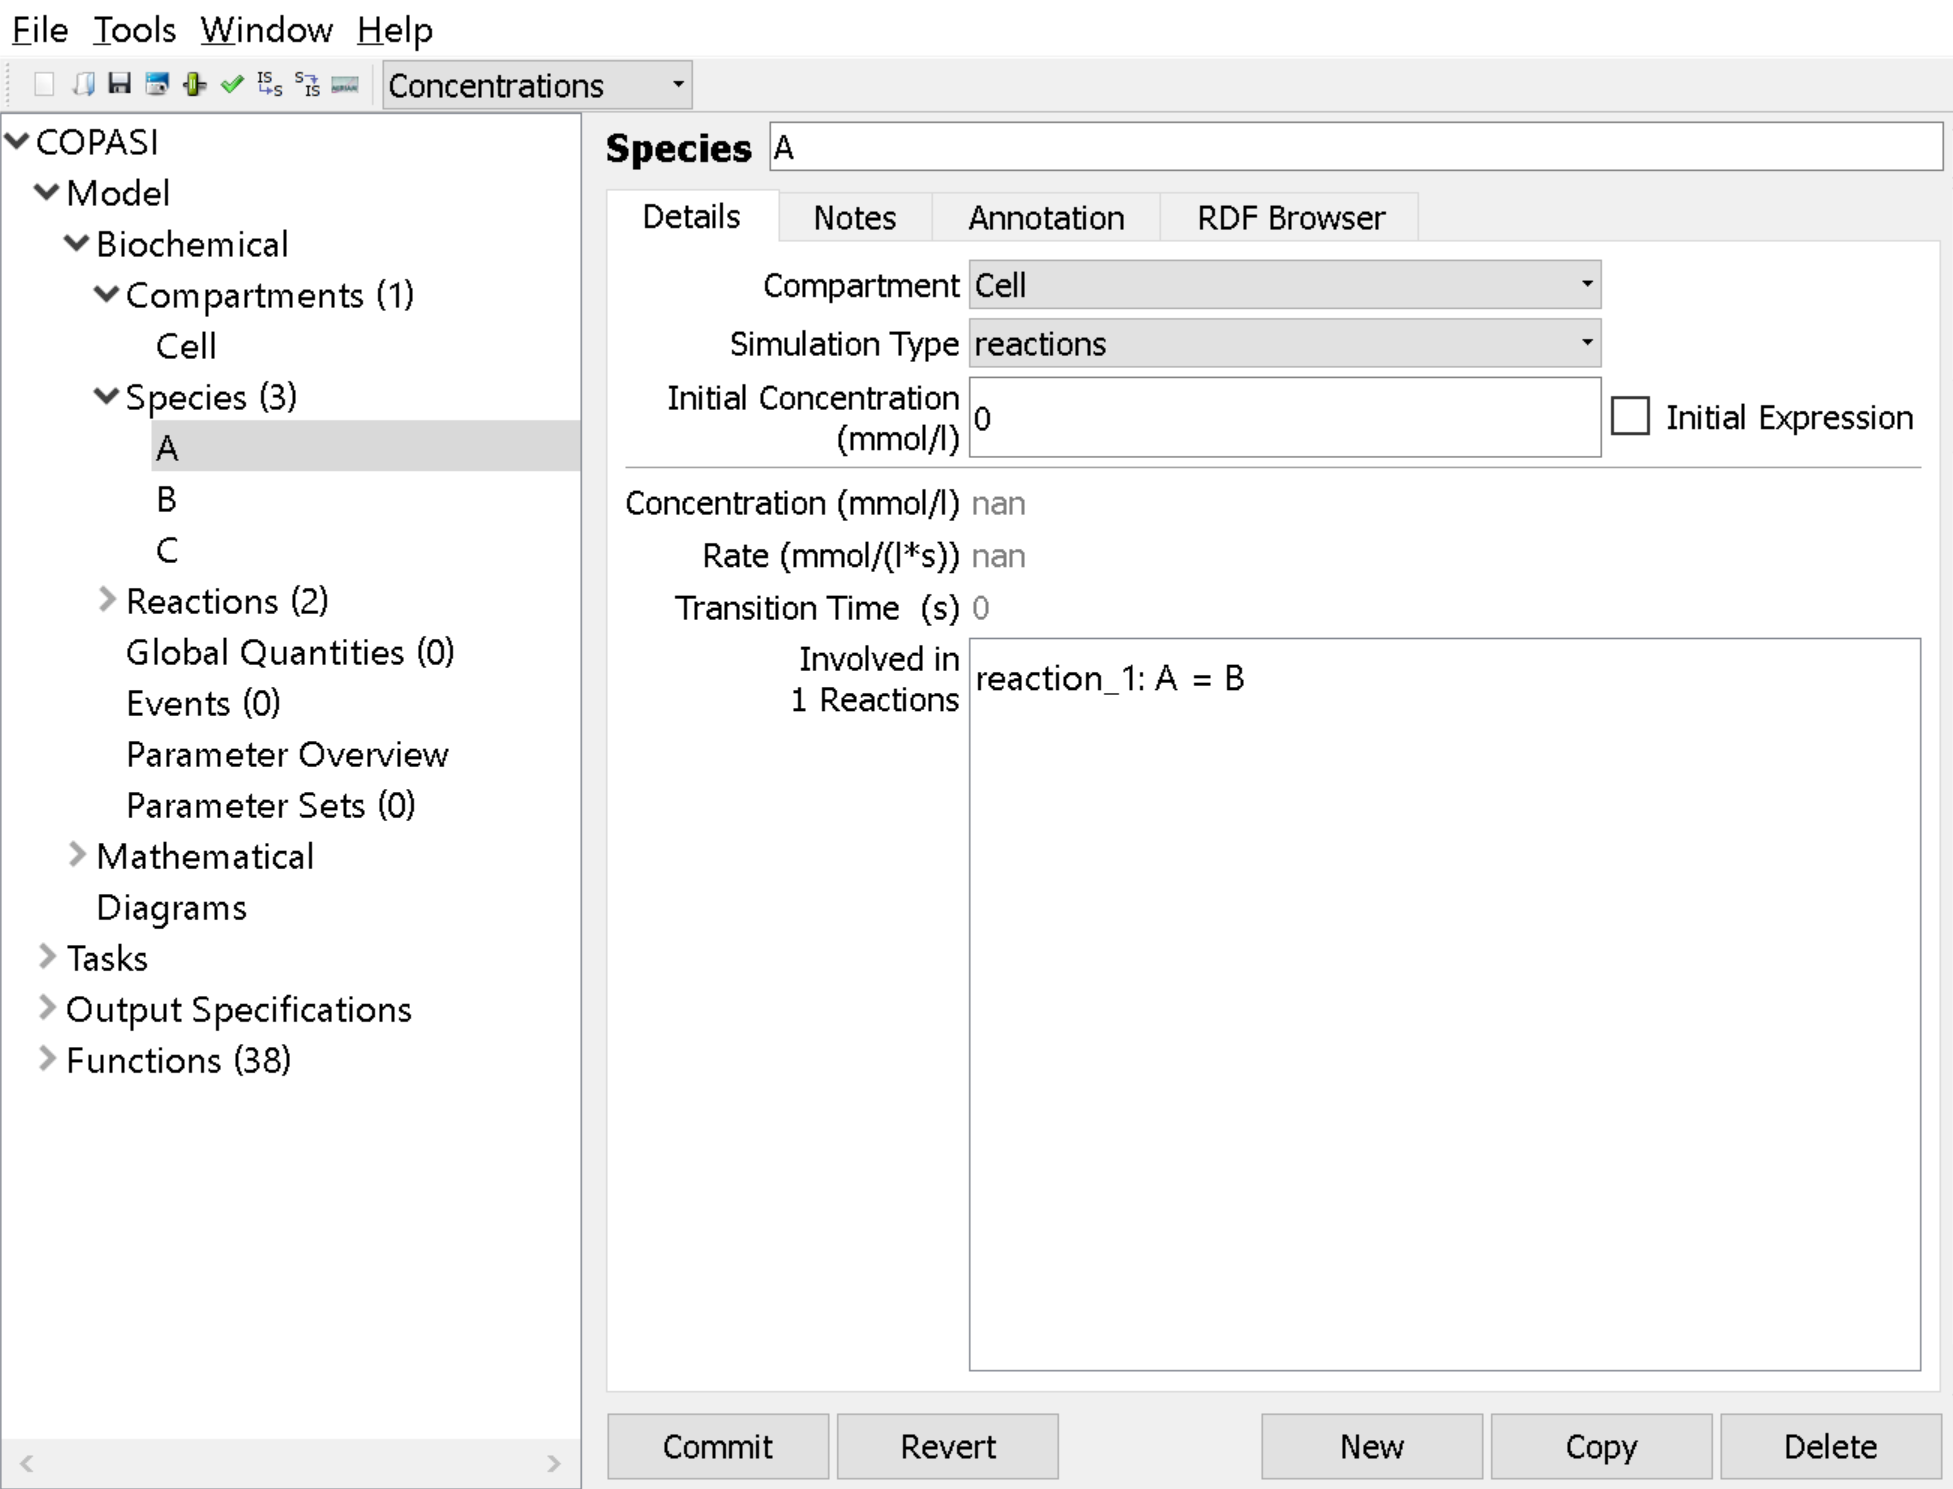
\includegraphics[height=5cm]{Images/5b.png}
			\caption{Species setup}
			\label{5png}
		\end{figure}
Similar to compartments, species are also generated automatically without defining the location of the species (compartment), initial concentration, and variability type. These values need to be assigned to each species.
\begin{enumerate} 
			\item In the \textbf{Object tree}, under \textbf{Species}, select species A.
			\item In the \textbf{Editor} pane, under \textbf{Details} tab, choose the \textbf{Compartment} of species A as \textbf{Cell}. 
			\item Choose the variability of species A (\textbf{Simulation Type}) as \textbf{reactions} from the drop-down menu.
			\item Enter \textbf{Initial Concentration} of species A (1 $\mu$mol).
			\item Repeat the steps a-d for each species.\\
		\end{enumerate}
	\end{enumerate}
Here we complete the model creation. Now an overview of the model can be seen under \textbf{Parameter Overview} in the \textbf{Object tree}. In \textbf{Parameter Overview}, we can modify (only) values of all parameters.
\subsection{Model Visualization-Figure~\ref{6png}}
	\begin{figure}[!htb]
		\centering
		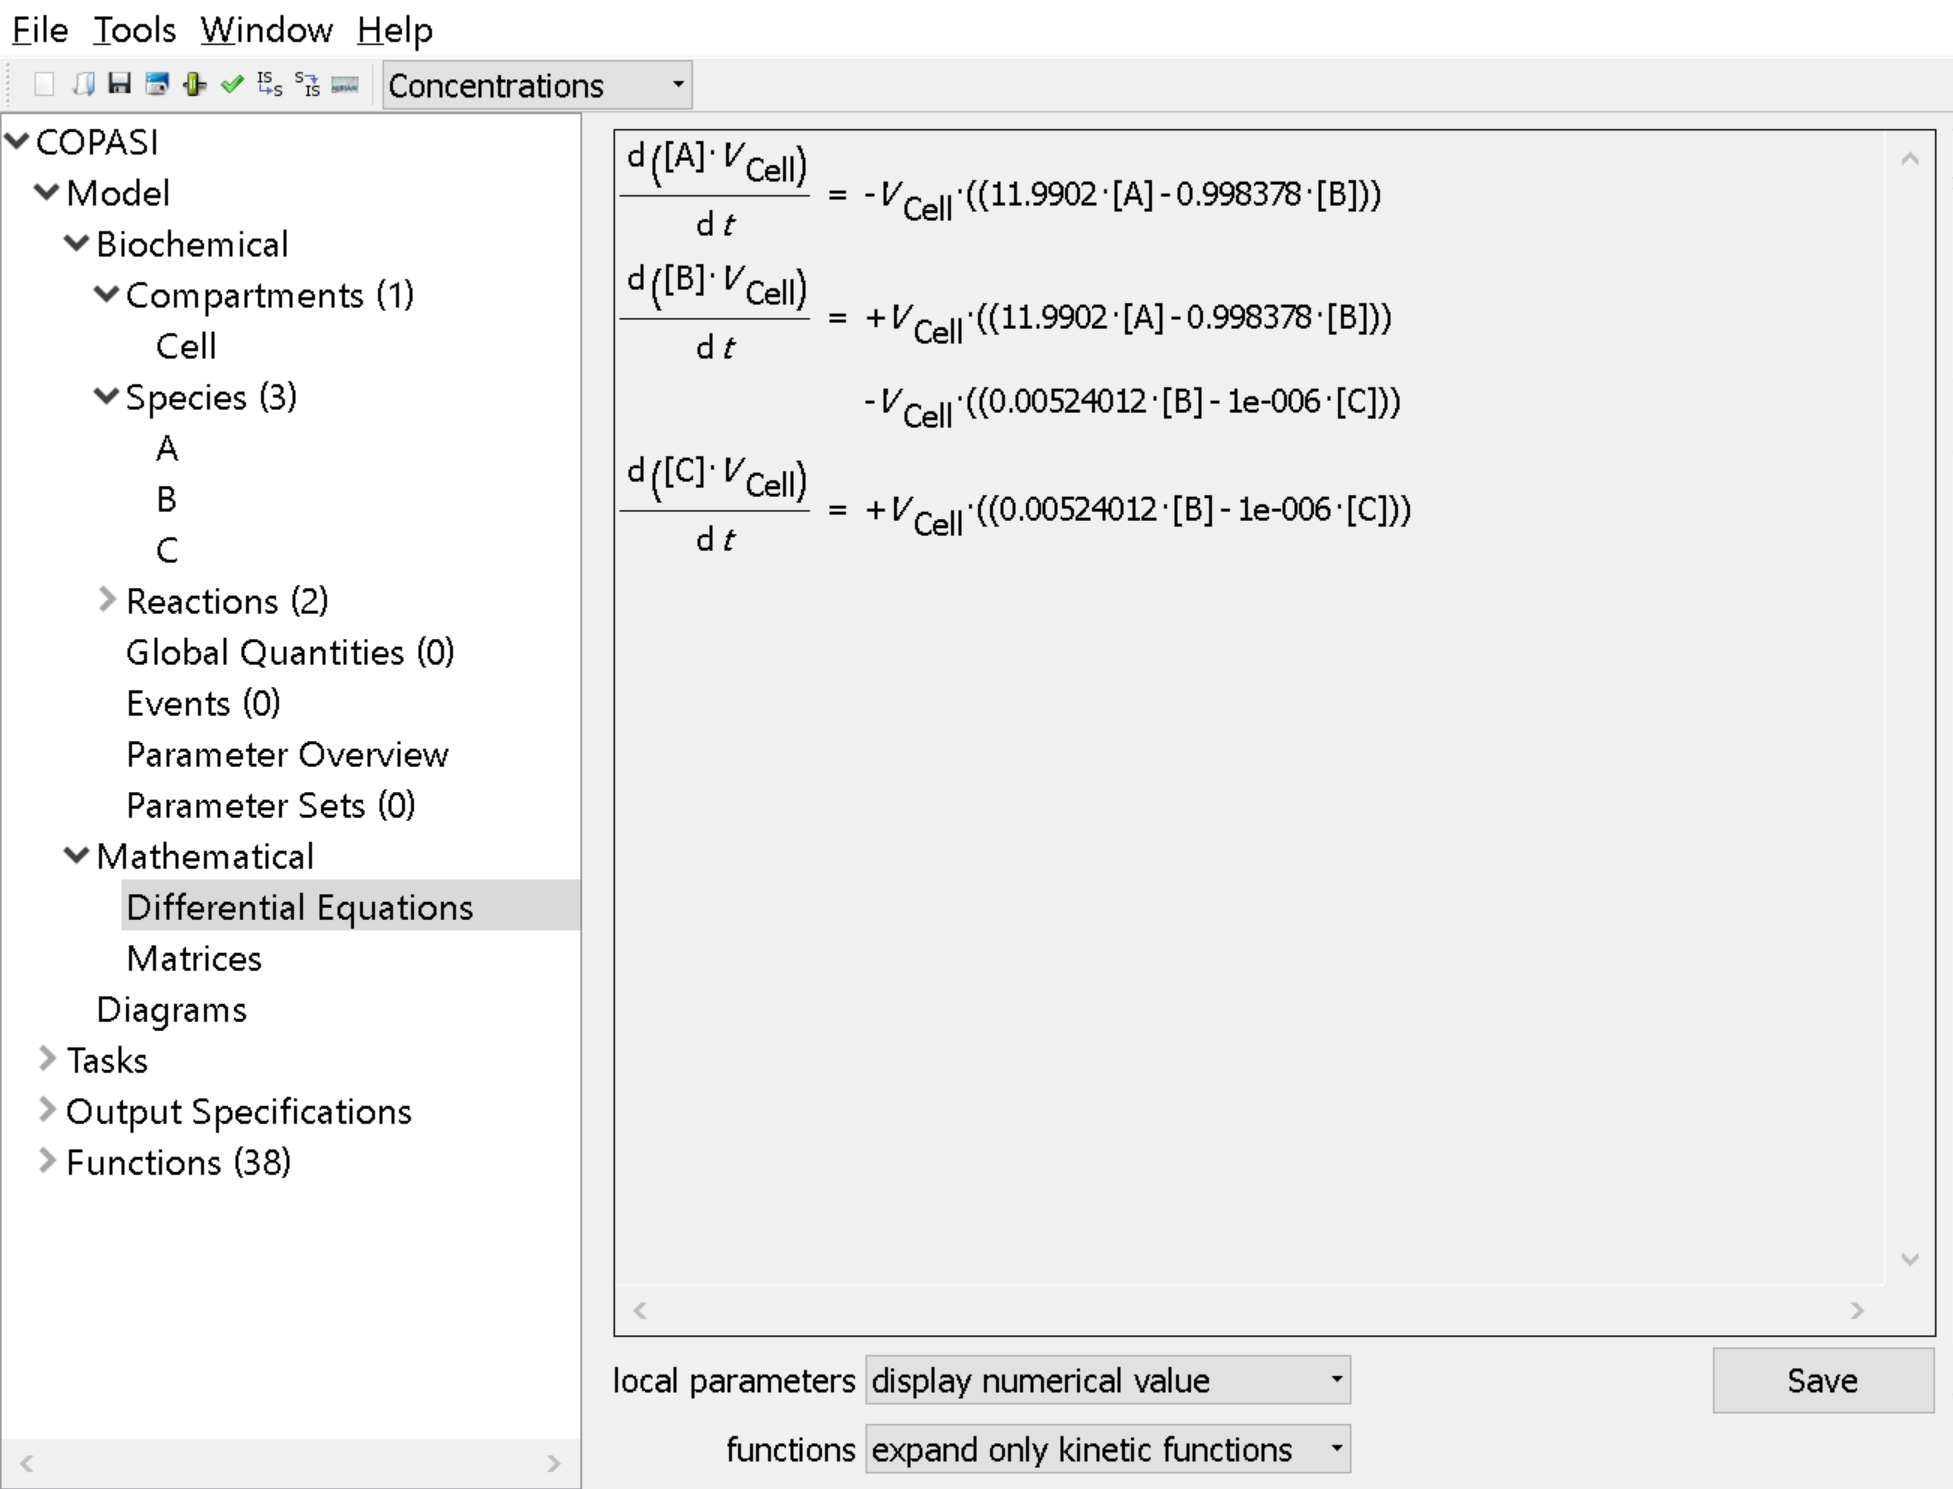
\includegraphics[height=5cm]{Images/6a.png}
		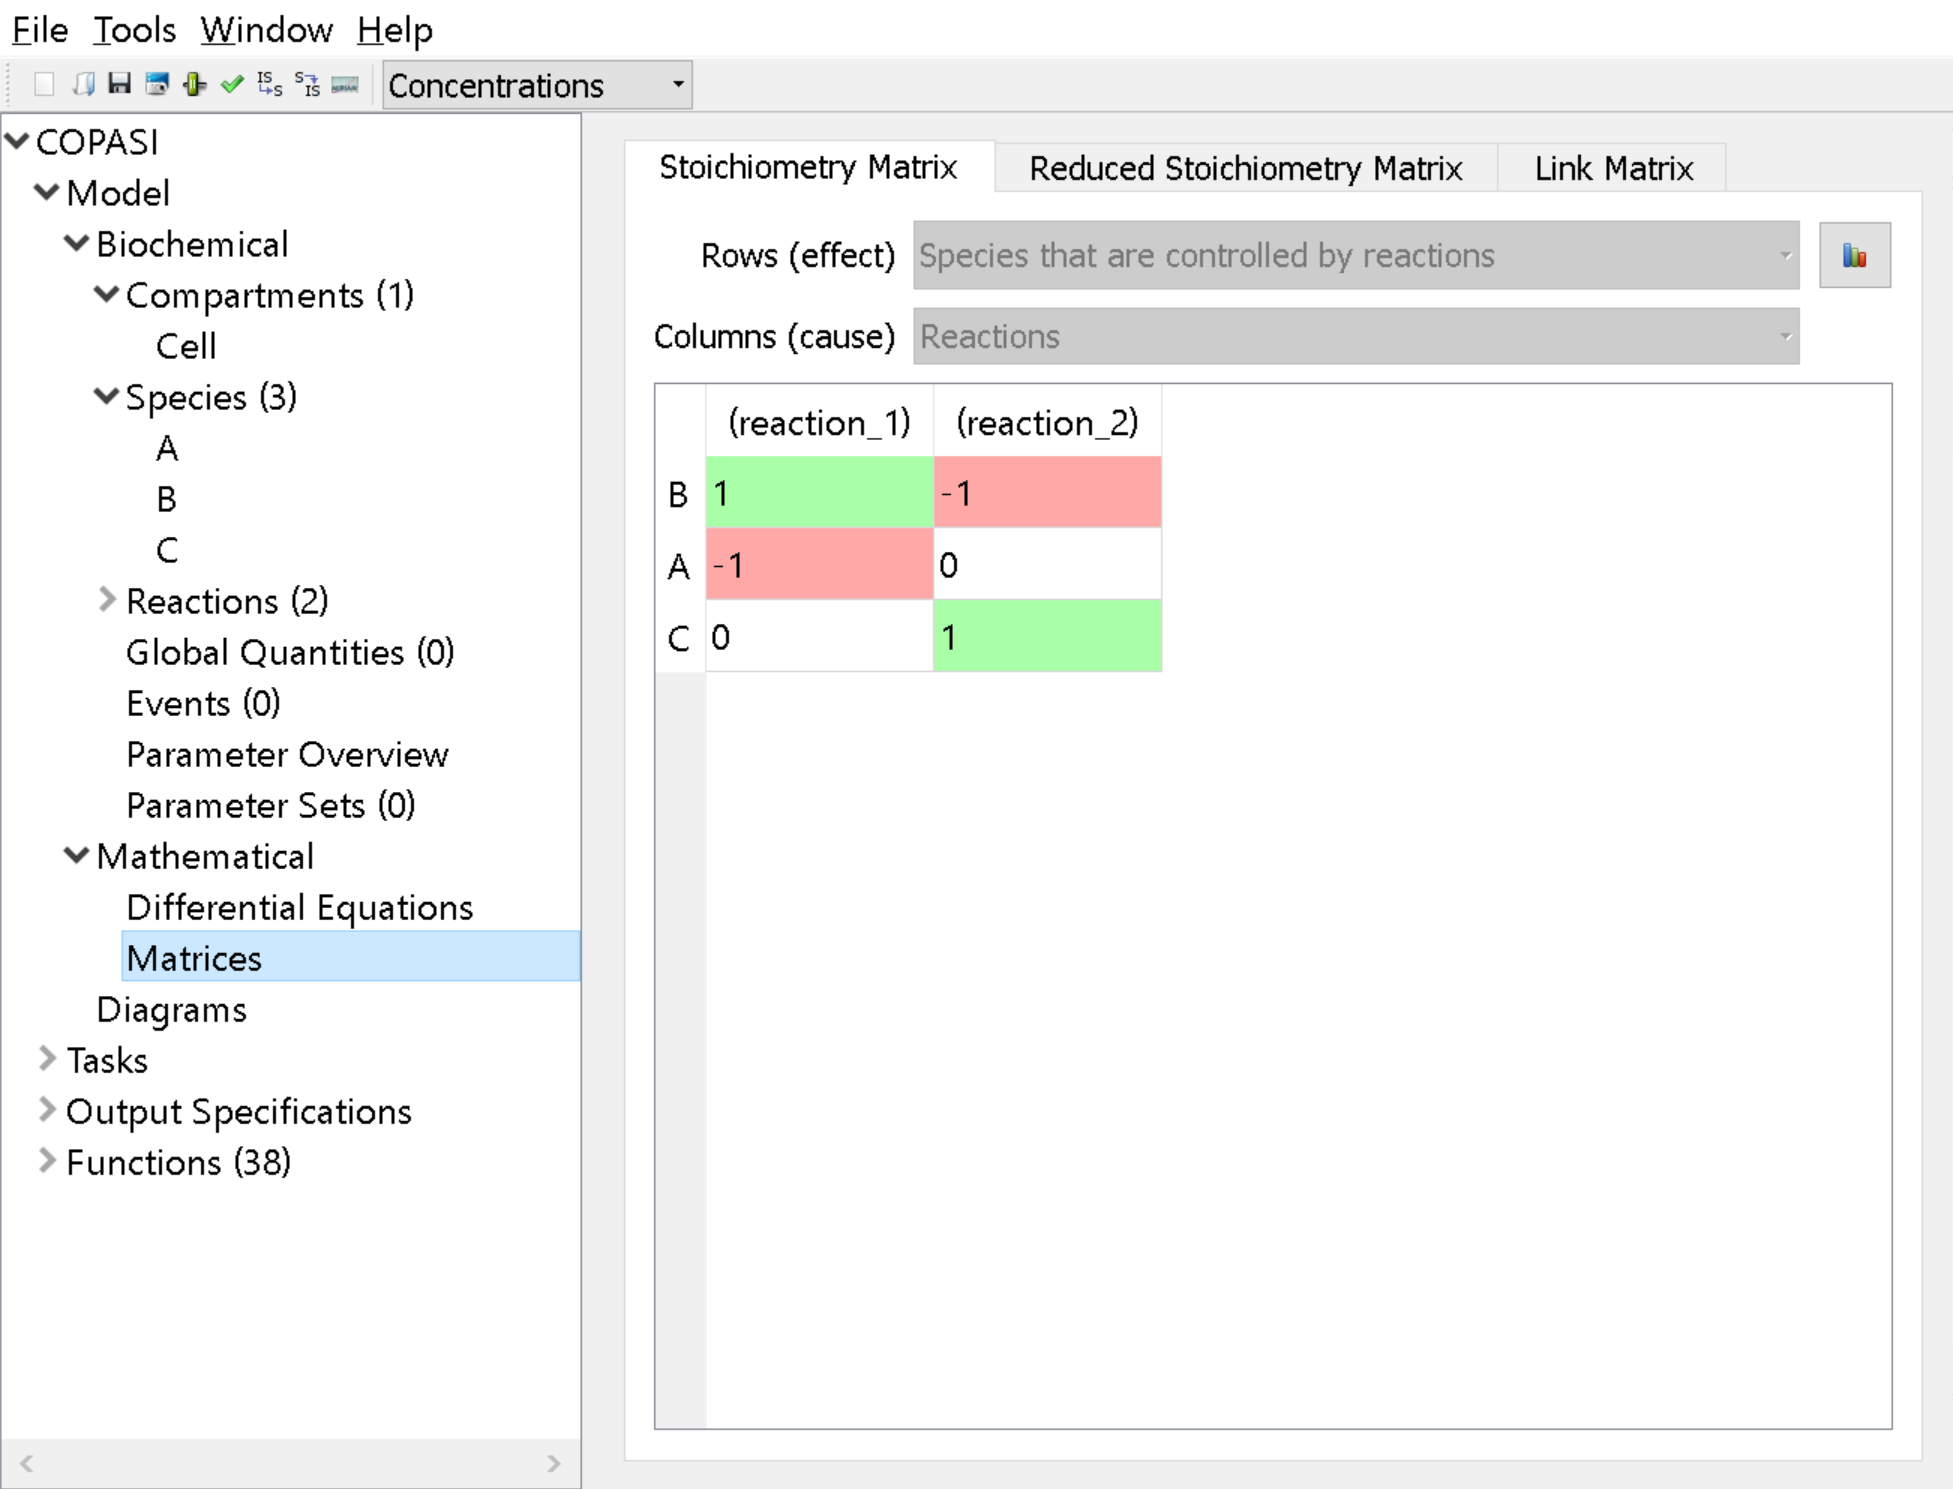
\includegraphics[height=5cm]{Images/6b.png}
		\caption{Mathematical model visualization}
		\label{6png}
	\end{figure}
    Once we set up the model, we can visualize the model mathematically by selecting \textbf{Mathematical} under \textbf{Model} in the \textbf{Object tree}. Mathematically, there are two ways to visualize the model. First, the model described in terms of differential equations which is a system of reaction rate equations (RREs) displayed in the Editor of \textbf{Differential Equations} under \textbf{Mathematical}. 
    

Second mathematical visualization comes in terms of stoichiometry matrix and possible reductions due to conservation laws.  In the \textbf{Object tree}, Under \textbf{Mathematical}, select \textbf{Matrices}. In the \textbf{Editor} pane, under \textbf{Stoichiometry Matrix} tab, we can see how the molecular population (discrete) changes due to different reactions.

	Other than mathematical visualization, we can also see the biochemical system as a network using \textbf{Diagrams} in the \textbf{Object tree}.
	
	\section{Tasks}
	In COPASI, analysis of biochemical models is grouped into multiple tasks. In each task, there are multiple ways to see results such as raw data, plots, and reports. 
	
	\subsection{Time-Course-Figure~\ref{7png}}
    One of the primary analysis of a biochemical system that is of common interest is the time evolution of the system. COPASI offers three types of methods, deterministic, stochastic and hybrid algorithms, to generate the time evolution.
\begin{figure}[!htb]
		\centering
		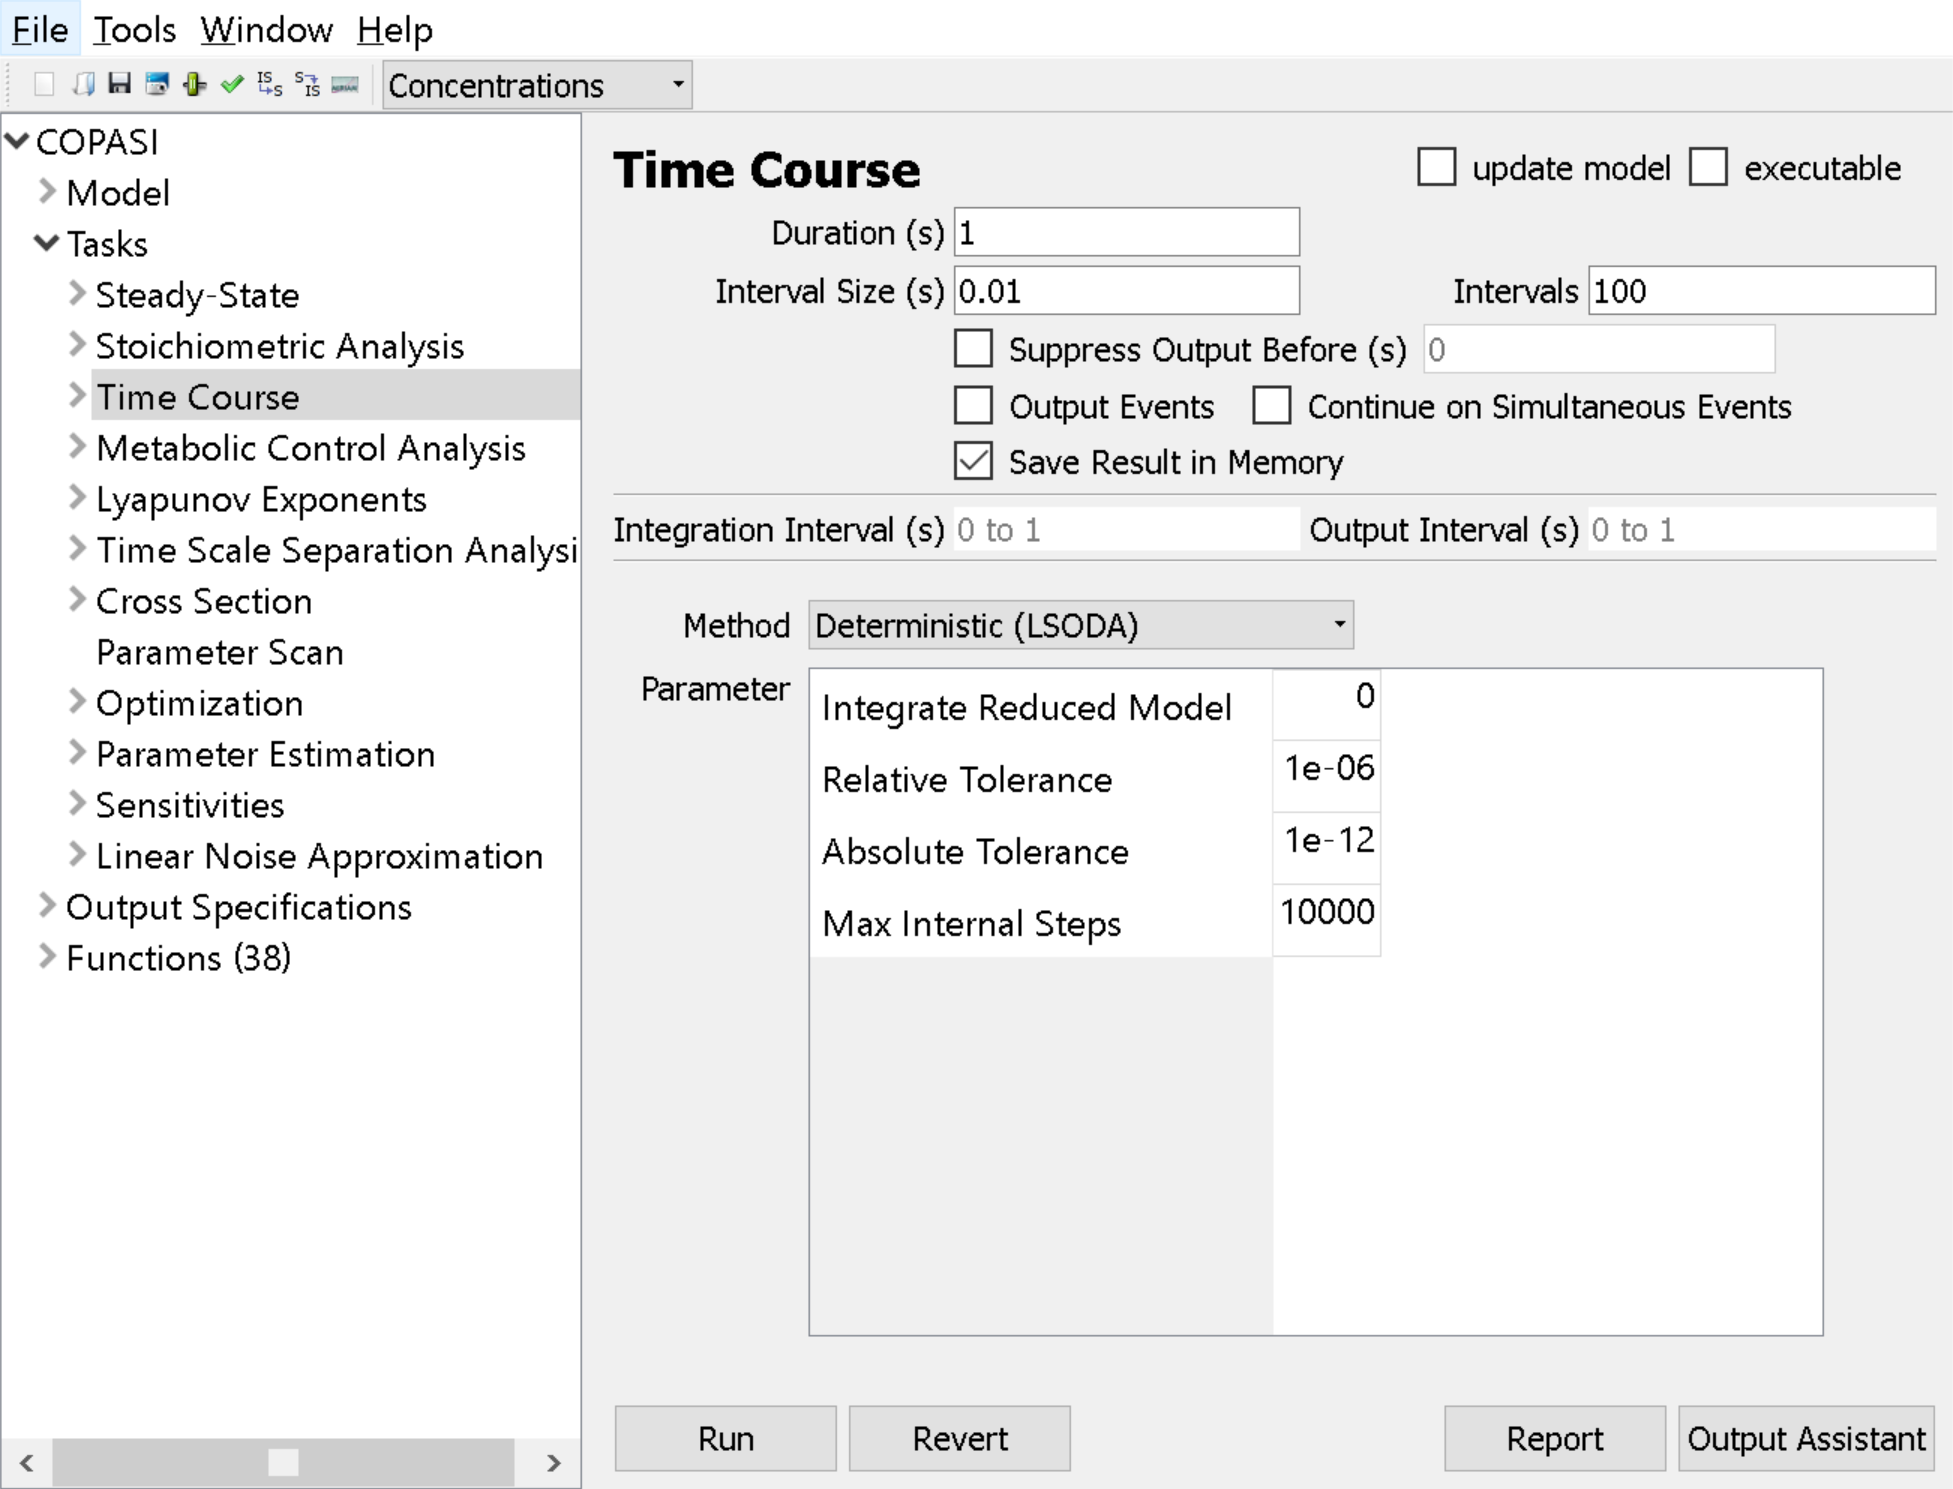
\includegraphics[height=8cm]{Images/7a.png}
		\caption{Time-Course}
		\label{7png}
	\end{figure}
	\subsubsection*{Set up}
	\begin{enumerate}[start=1]\def\makelabel{\textbf{Step}~}
		\item In the \textbf{Object tree}, under \textbf{Tasks}, select \textbf{Time Course}.
		\item In the \textbf{Editor} pane, choose the \textbf{Duration} of the analysis (\textbf{1})
		\item Choose the \textbf{Interval Size} ($\textbf{0.001}$) or \textbf{Intervals} (\textbf{1000}). Only one of these needs to be entered. Other quantity will update automatically using the parameter in \textbf{Duration}.
		\item (optional) Check \textbf{Suppress Output Before} and type from what time point need to analyze the model
		\item Check \textbf{Save Result in Memory}
		\item Choose the \textbf{Method} of analysis (\textbf{Deterministic (LSODA)})
		\item select \textbf{Run}
	\end{enumerate}
	\subsubsection*{Results-Figure~\ref{Result1}}			\begin{figure}[!htb]
	\centering
	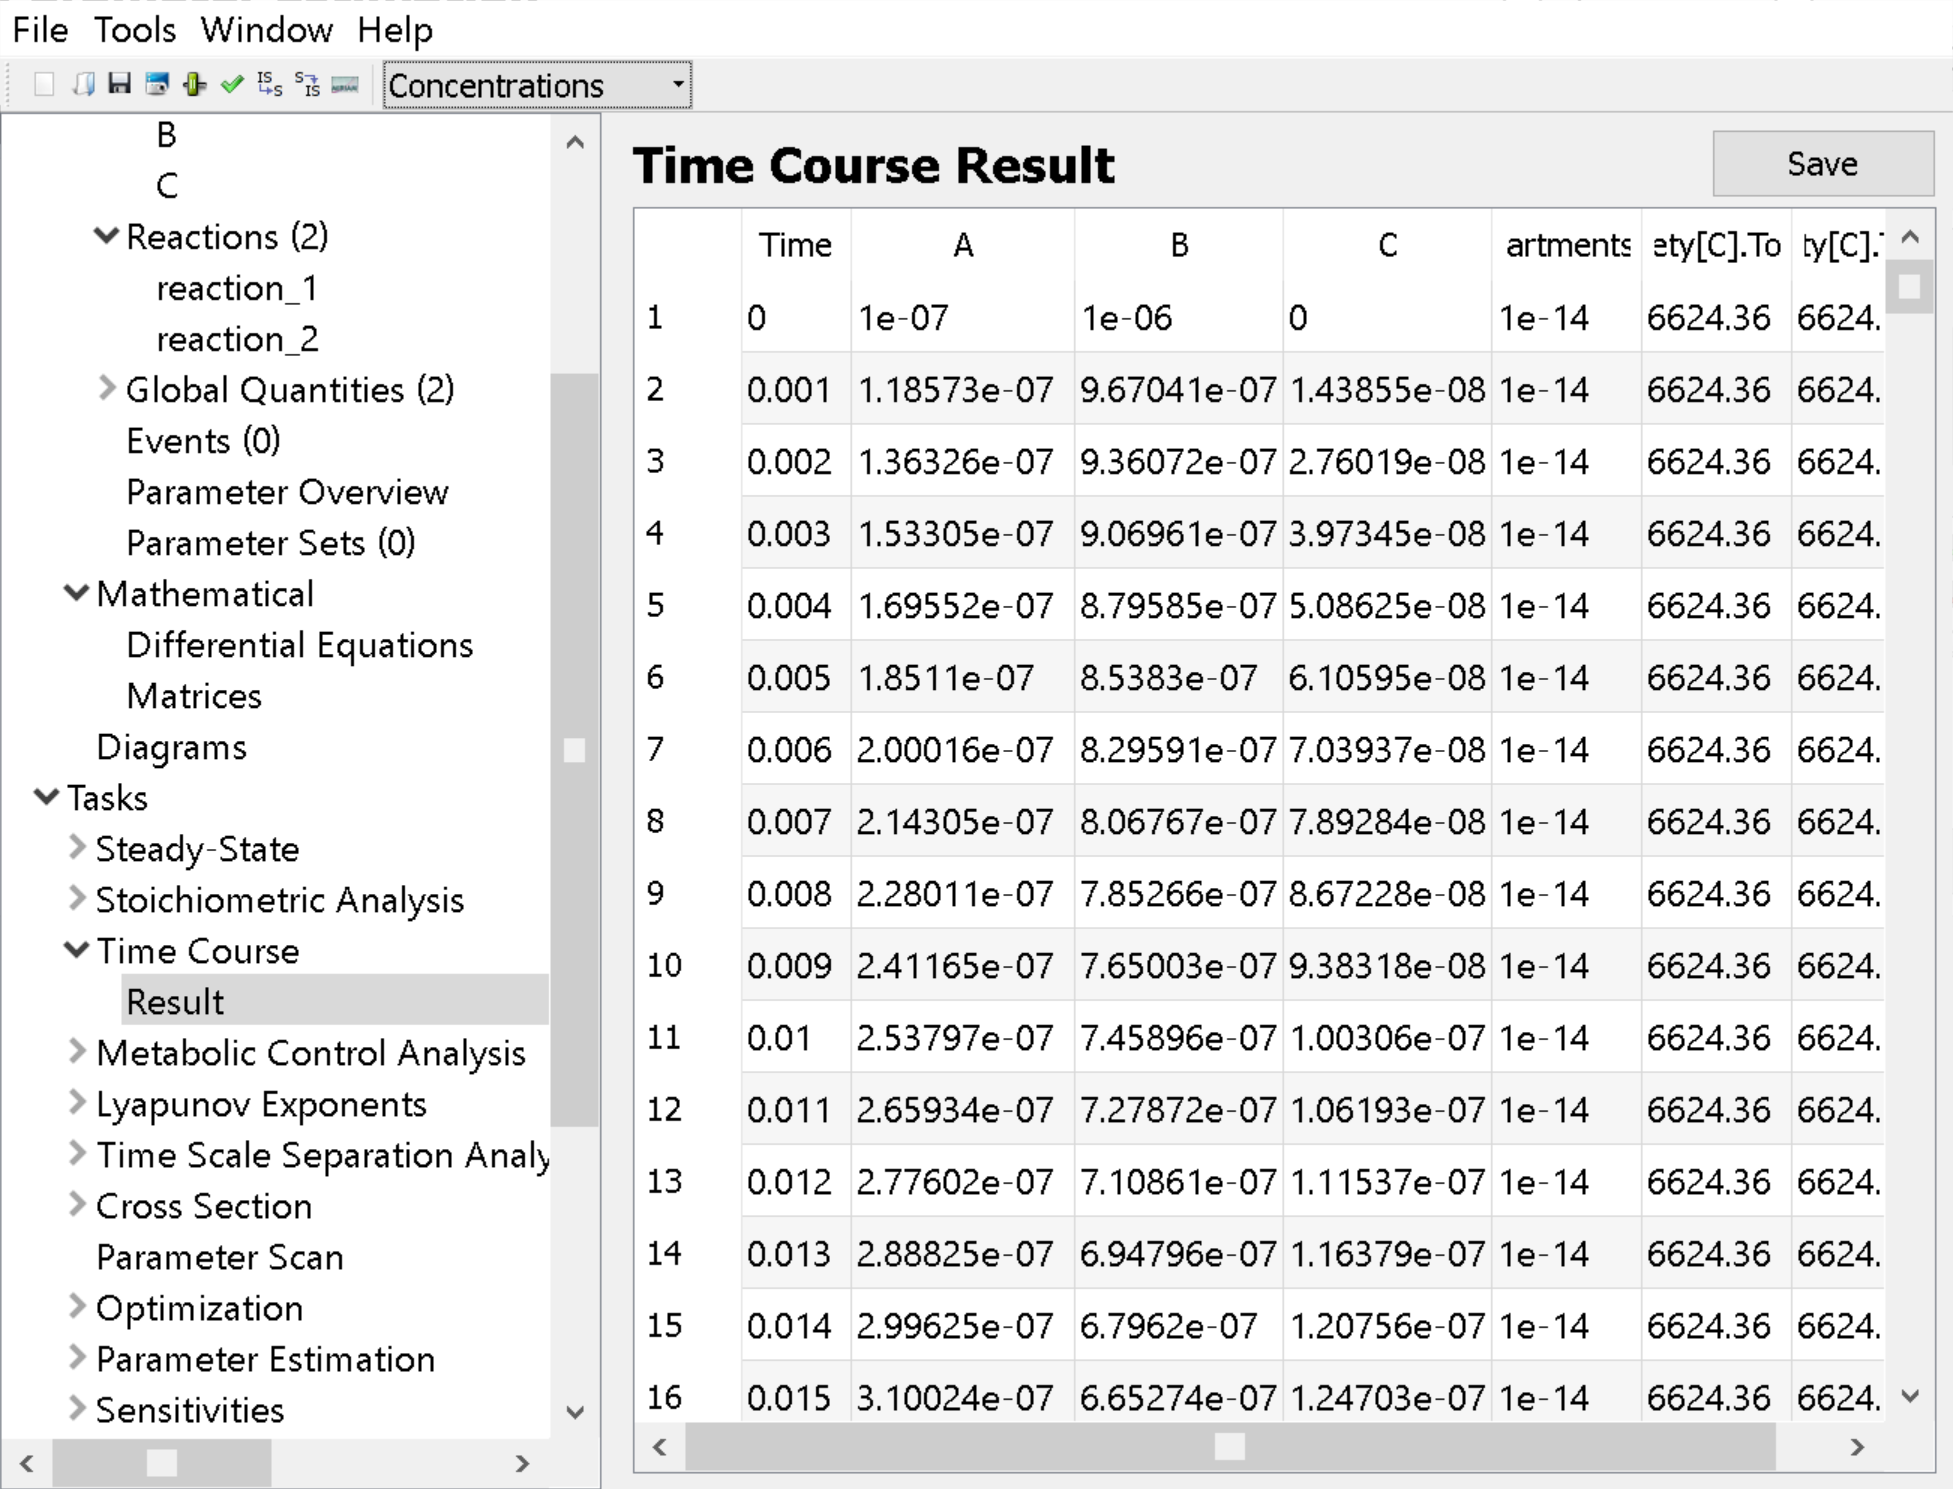
\includegraphics[height=8cm]{Images/R1a.png}		
	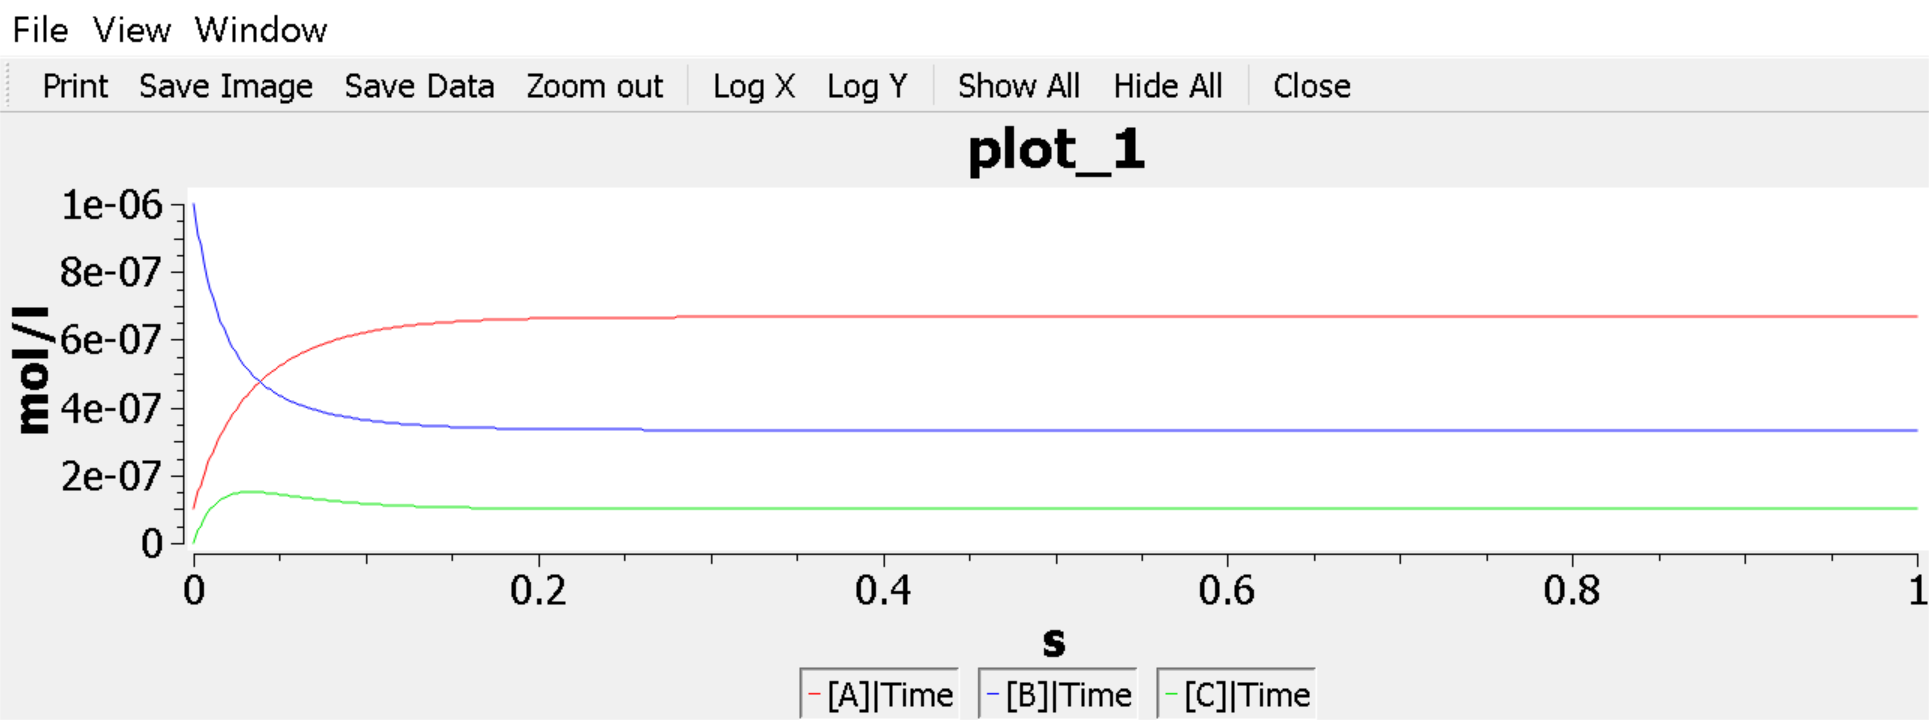
\includegraphics[height=5cm]{Images/R1b.png}
	\caption{Result plot}
	\label{Result1}
	\end{figure}
	There are multiple ways to visualize the result. First,  the raw data of the simulation in \textbf{Results} under \textbf{Time Course}. Other options are generating \textbf{Plots} and \textbf{Reports} of the result using \textbf{Output Assistant}. 
	
	\subsubsection{Plot-Figure~\ref{8png}}
	There are multiple predefined templates of plots are available in COPASI, which is capable of generating plots for most of the situations. However, we can also create customized plots if necessary.
	\begin{figure}[!htb]
		\centering
		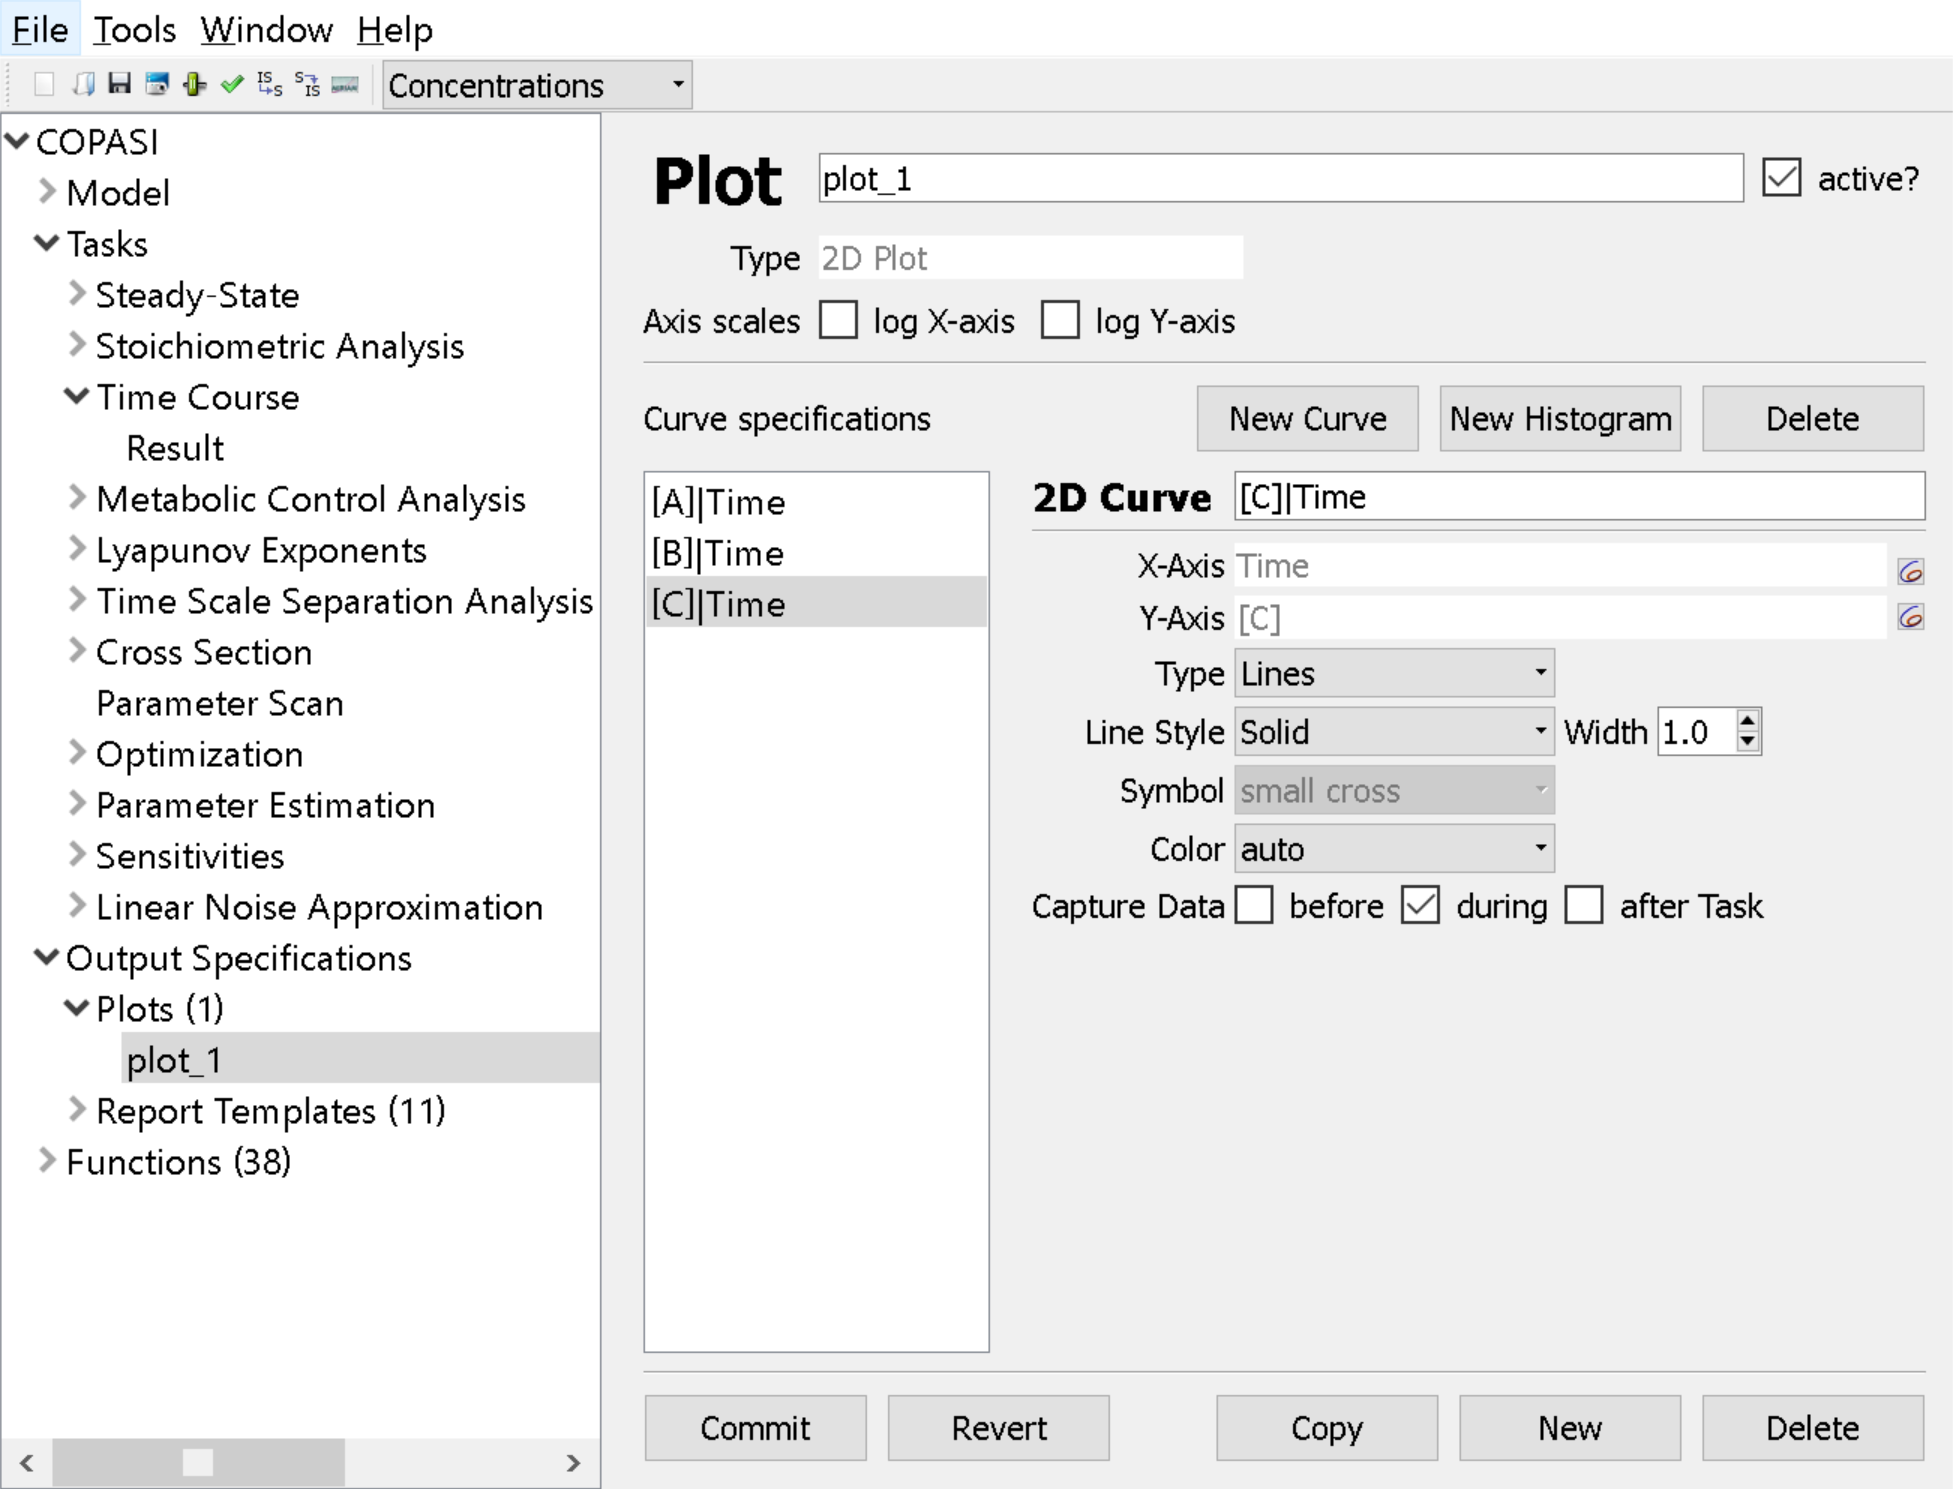
\includegraphics[height=5cm]{Images/8a.png}
		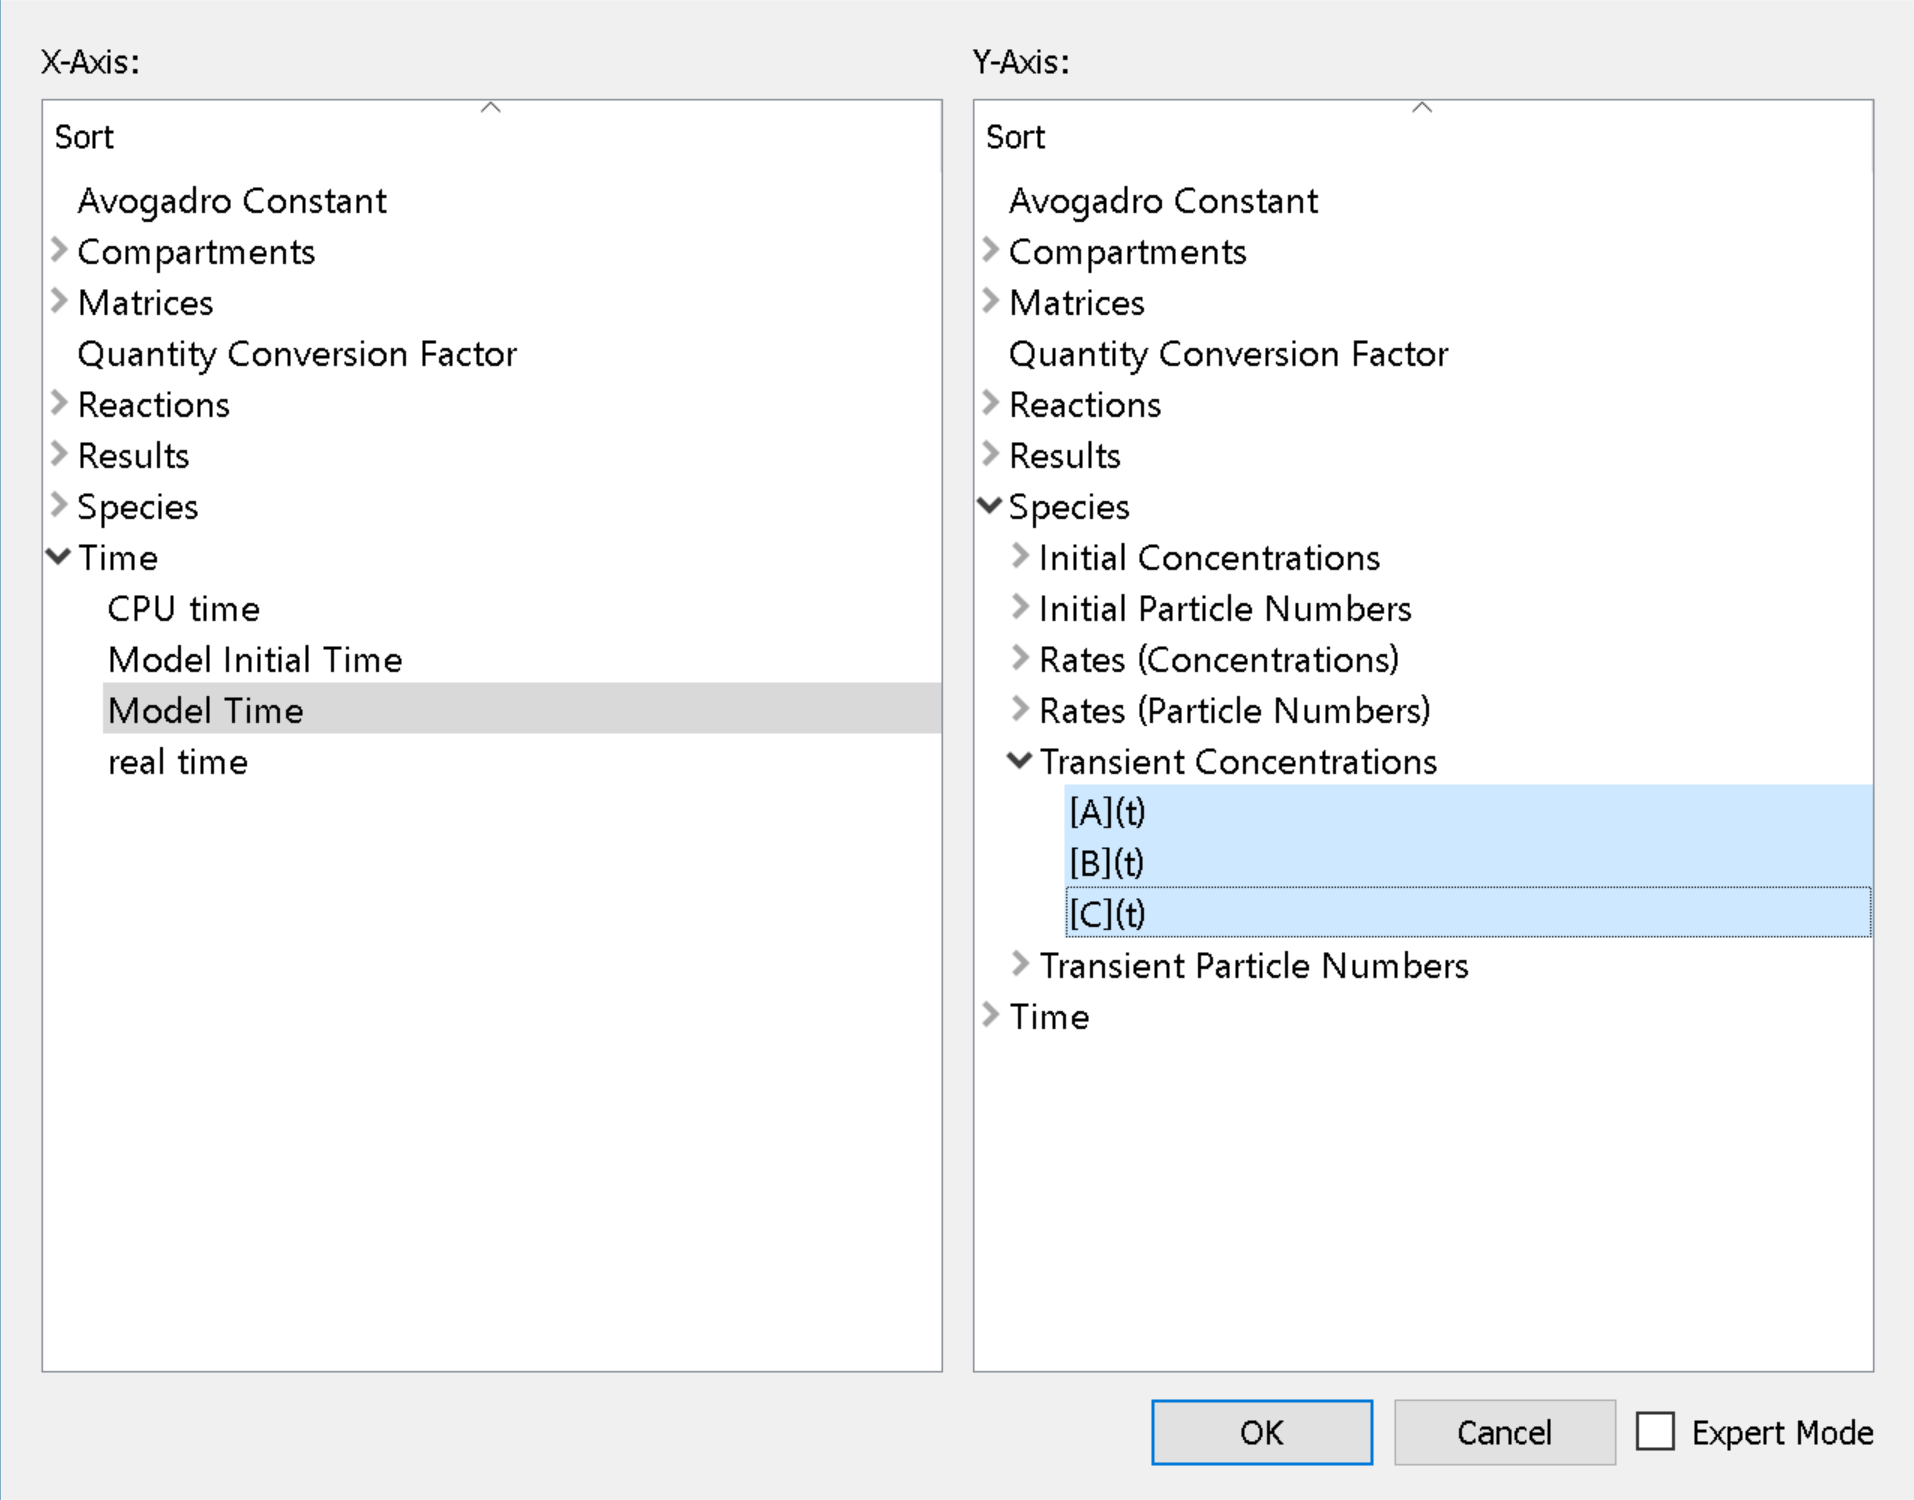
\includegraphics[height=5cm]{Images/8b.png}
		\caption{Plot setup}
		\label{8png}
	\end{figure}
	\begin{enumerate}[start=1]\def\makelabel{\textbf{Step}~}
		\item In the \textbf{Object tree}, Under \textbf{Output Specifications}, select \textbf{Plots}
		\item In the \textbf{Editor} pane, Click on \textbf{New}
		\item Double click on newly created plot \textbf{plot\_1}
		\item (optional) Change name of the plot (\textbf{Time Course Analysis})
		\item Choose the type of plot (\textbf{Curve} or Histogram) by selecting \textbf{New Curve} or \textbf{New Histogram}. Select \textbf{New Curve} for now.
		\item In the pop-up box, select the \textbf{X} and \textbf{Y} axis elements. In the column \textbf{X-Axis}, expand \textbf{Time} and select \textbf{Model Time}. In the column \textbf{Y-Axis}, expand \textbf{Species} and then expand \textbf{Transient Concentrations} and choose the species which needs to show in the plot (\textbf{[A](t), [B](t), [C](t)}) and select \textbf{OK}.\\
	\end{enumerate}
	Once we created a plot output \textbf{Run} the \textbf{Task -Time Course} again to see the plot generated from the result.
	
	\subsubsection{Reports-Figure~\ref{9png}}
	Reports are a customized way of exporting raw data of the analysis. In reports, we can choose the variables of interest.
	\begin{figure}[!htb]
		\centering
		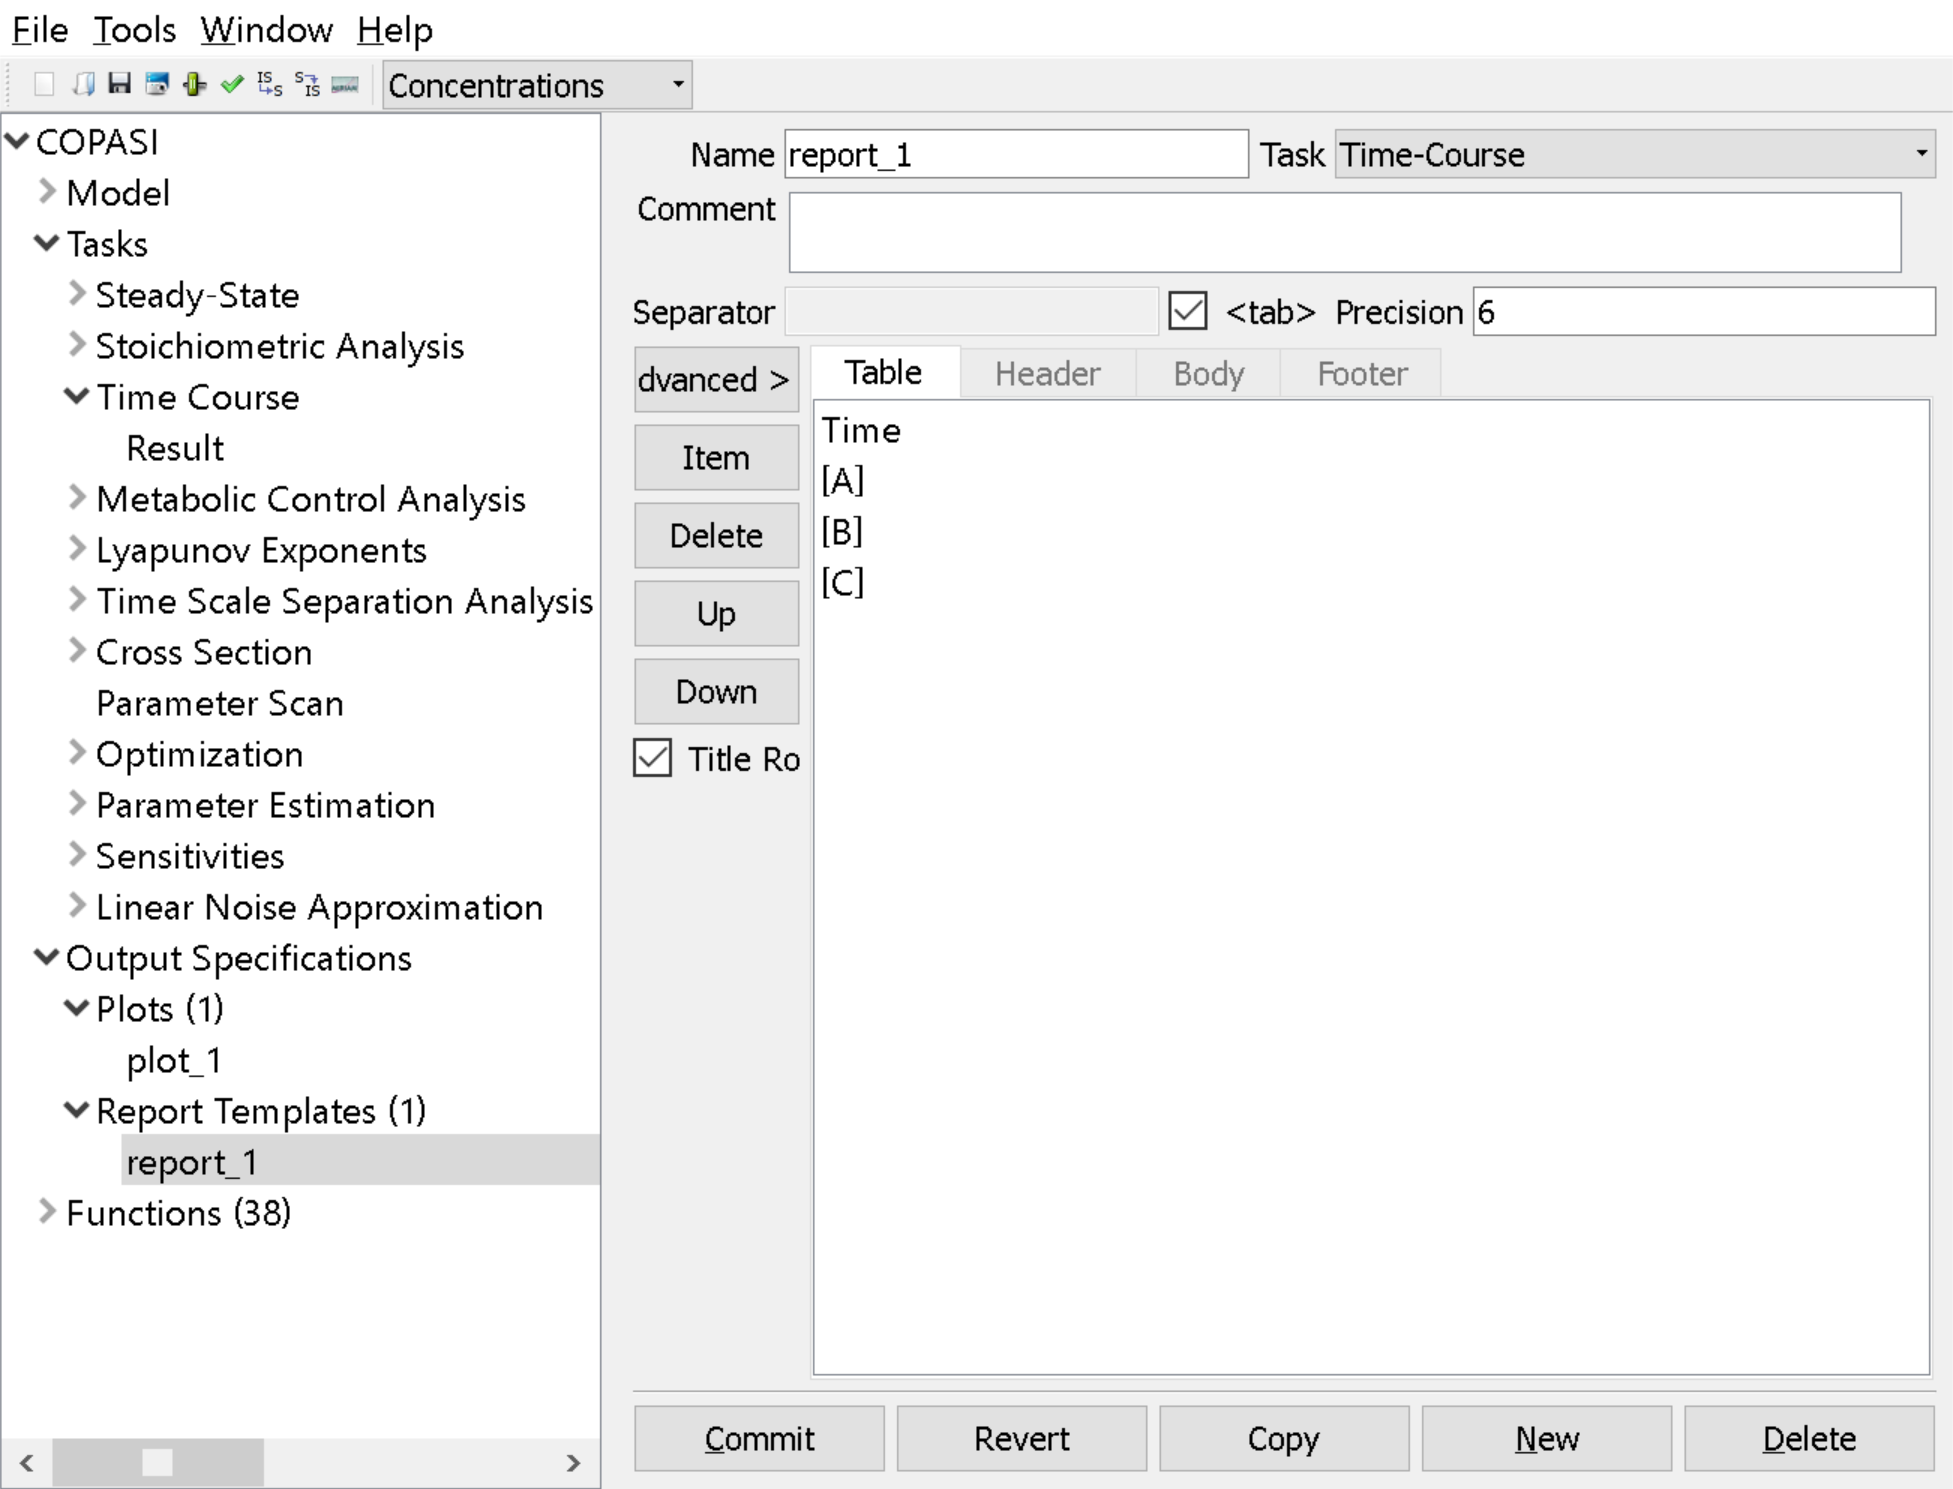
\includegraphics[height=5cm]{Images/9a.png}
		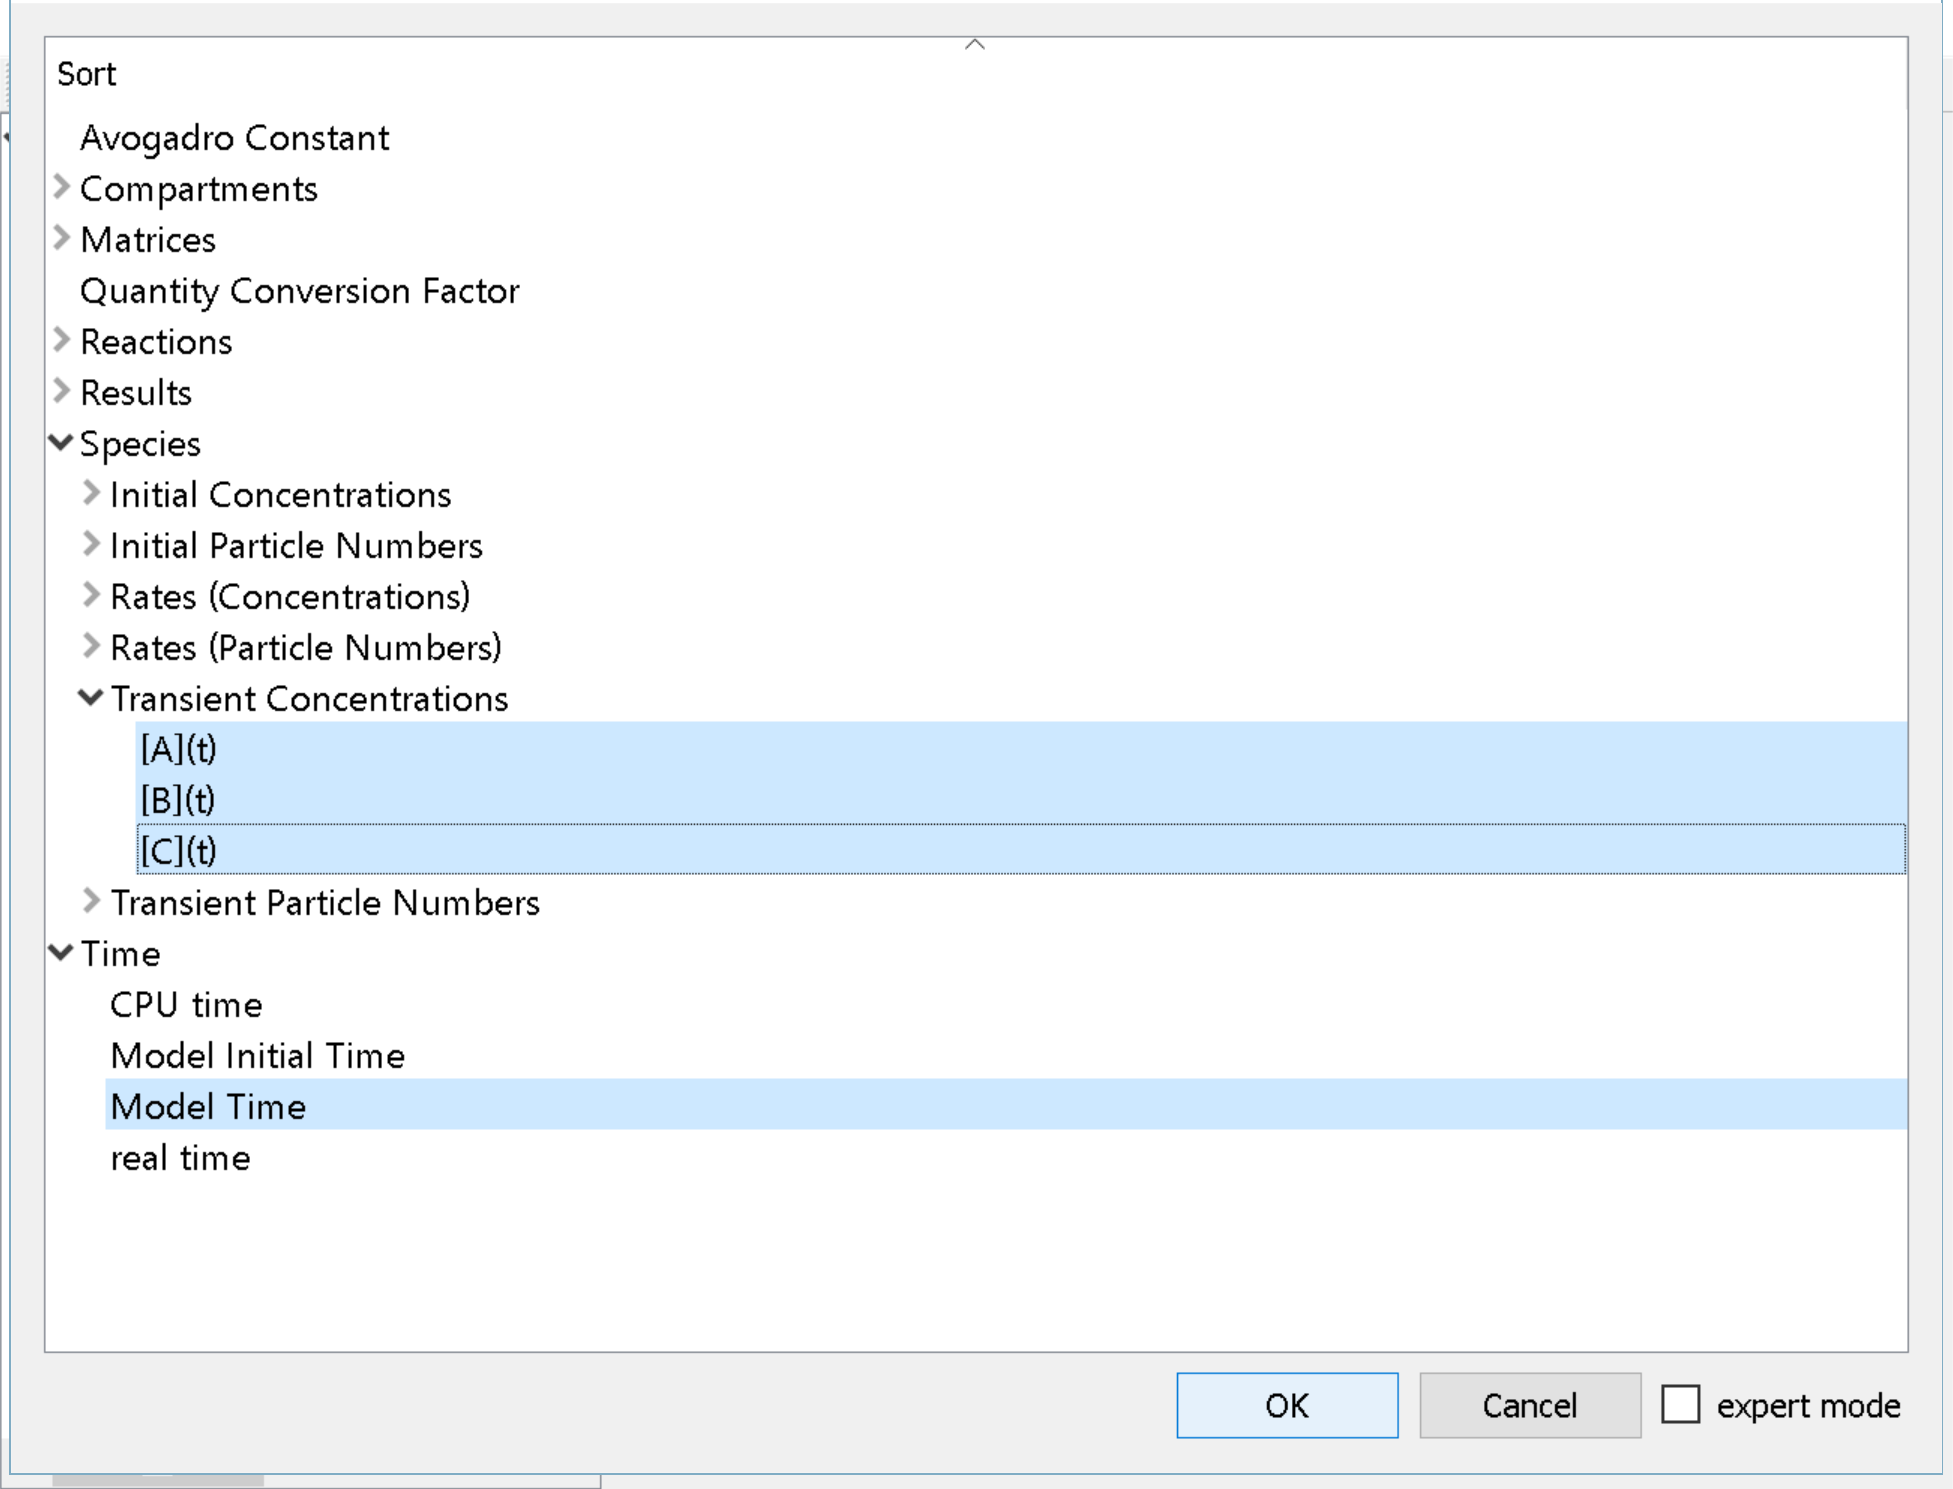
\includegraphics[height=5cm]{Images/9b.png}
		\caption{Report setup}
		\label{9png}
	\end{figure}
	\begin{enumerate}[start=1]\def\makelabel{\textbf{Step}~}
		\item In the \textbf{Object tree}, Under \textbf{Output Specifications}, select \textbf{Reports}
		\item In the \textbf{Editor} pane, Click on \textbf{New}
		\item Double click on newly created report \textbf{report\_1}
		\item (optional) Change \textbf{Name} of the Report (\textbf{Time Course Analysis Report})
		\item Choose the \textbf{Task} next to \textbf{Name} for which the report needs to be generated (\textbf{Time Course})
		\item Select \textbf{Item} in the \textbf{Editor} pane to select variables in the report.
		\item In the pop-up box, expand \textbf{Species} and then expand \textbf{Transient Concentrations} and choose the species which needs to show in the report (\textbf{[A](t), [B](t), [C](t)}). Then expand \textbf{Time} and select \textbf{Model Time} (use Control/Command button to select multiple items). Finally select \textbf{OK}.\\
		%\end{enumerate}
		Note: Unlike plots, reports are needed to be saved onto a text file. Therefore we need to create/select a text file to save the results. Even if the type of reports are same, we need to generate different text files for different \textbf{Tasks}.
		%\begin{enumerate}[start=1]\def\makelabel{\textbf{Step}~}
		\item (For the \textbf{Time Course} task) go to \textbf{Time Course} and in the \textbf{Editor} pane, click on \textbf{Report} from the right bottom.
		\item From the pop-up box, type the location of the \textbf{Filename}. This can be done using clicking on the \textbf{file chooser} icon next to the cell corresponding to \textbf{Filename} (\textbf{Report-Time Course Linear.txt}).
		\item (optional) Check \textbf{Append}, if we wish to keep all the result of repeated trials of the analysis.\\
	\end{enumerate} 
	
	\textbf{Note}: There are many inbuilt plot and report templates which can be used to generate plots and reports. This can be accessed through \textbf{Output Assistant} which is available in the \textbf{Editor} pane of all \textbf{Tasks} listed in the \textbf{Object tree}.
	
	\section{Sensitivity Analysis-Figure~\ref{11png}}
	Some parameters of the system may be highly sensitive to the evolution of the system and some may not. These sensitive characteristics are used to optimize the model using reduction methods. COPASI's \textbf{Sensitivities} task is used to quantify the parameter sensitivities.
	\begin{figure}[!htb]
		\centering
		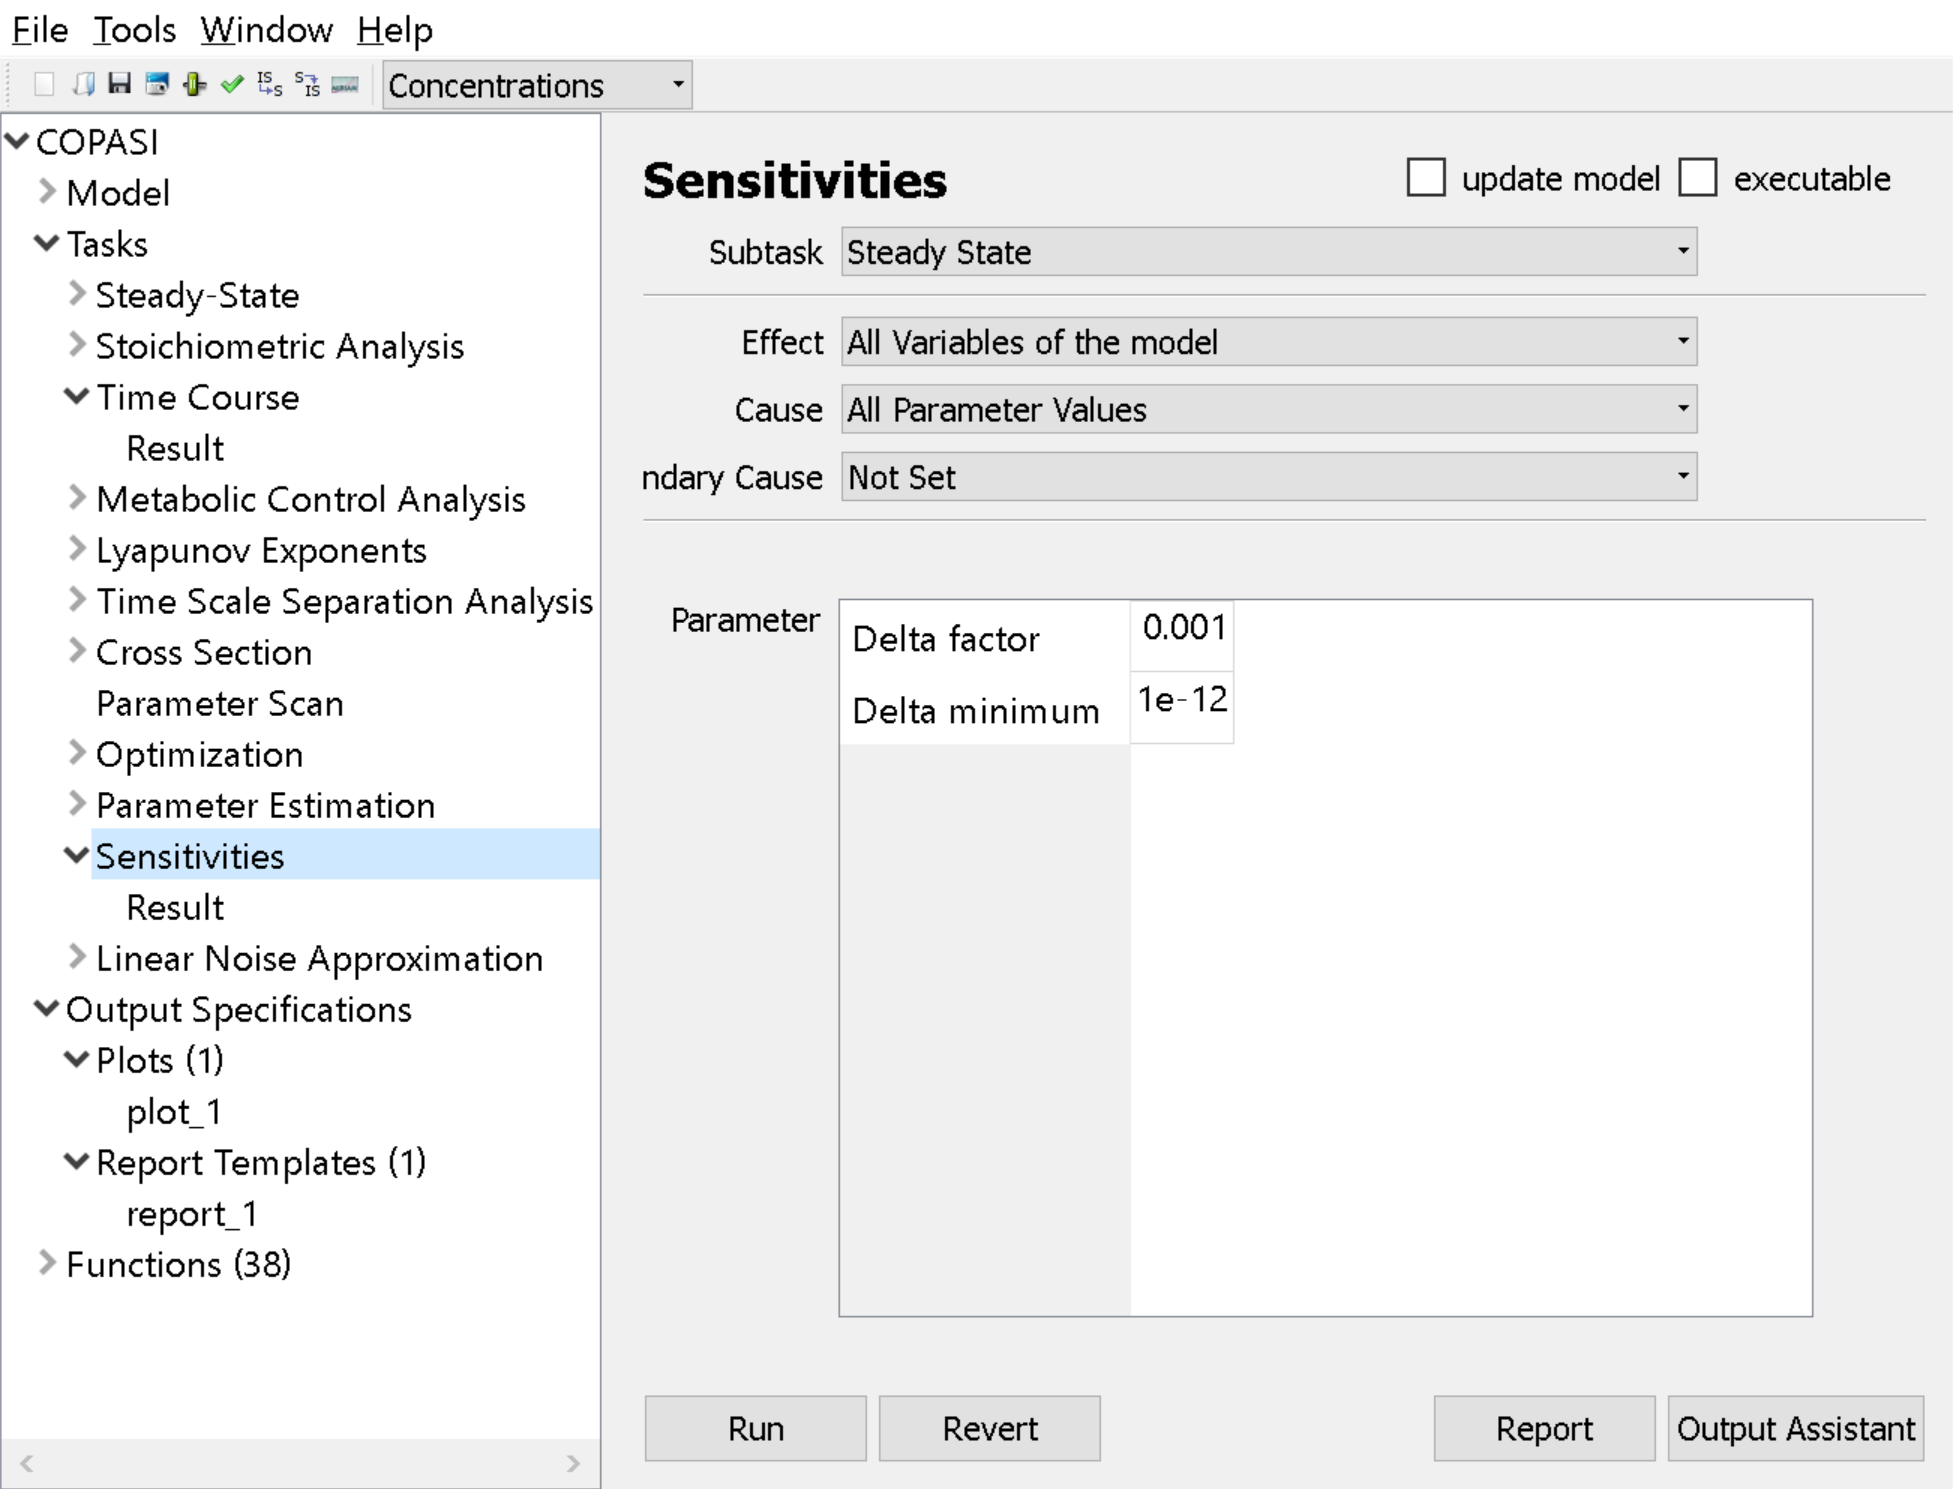
\includegraphics[height=5cm]{Images/11a.png}
		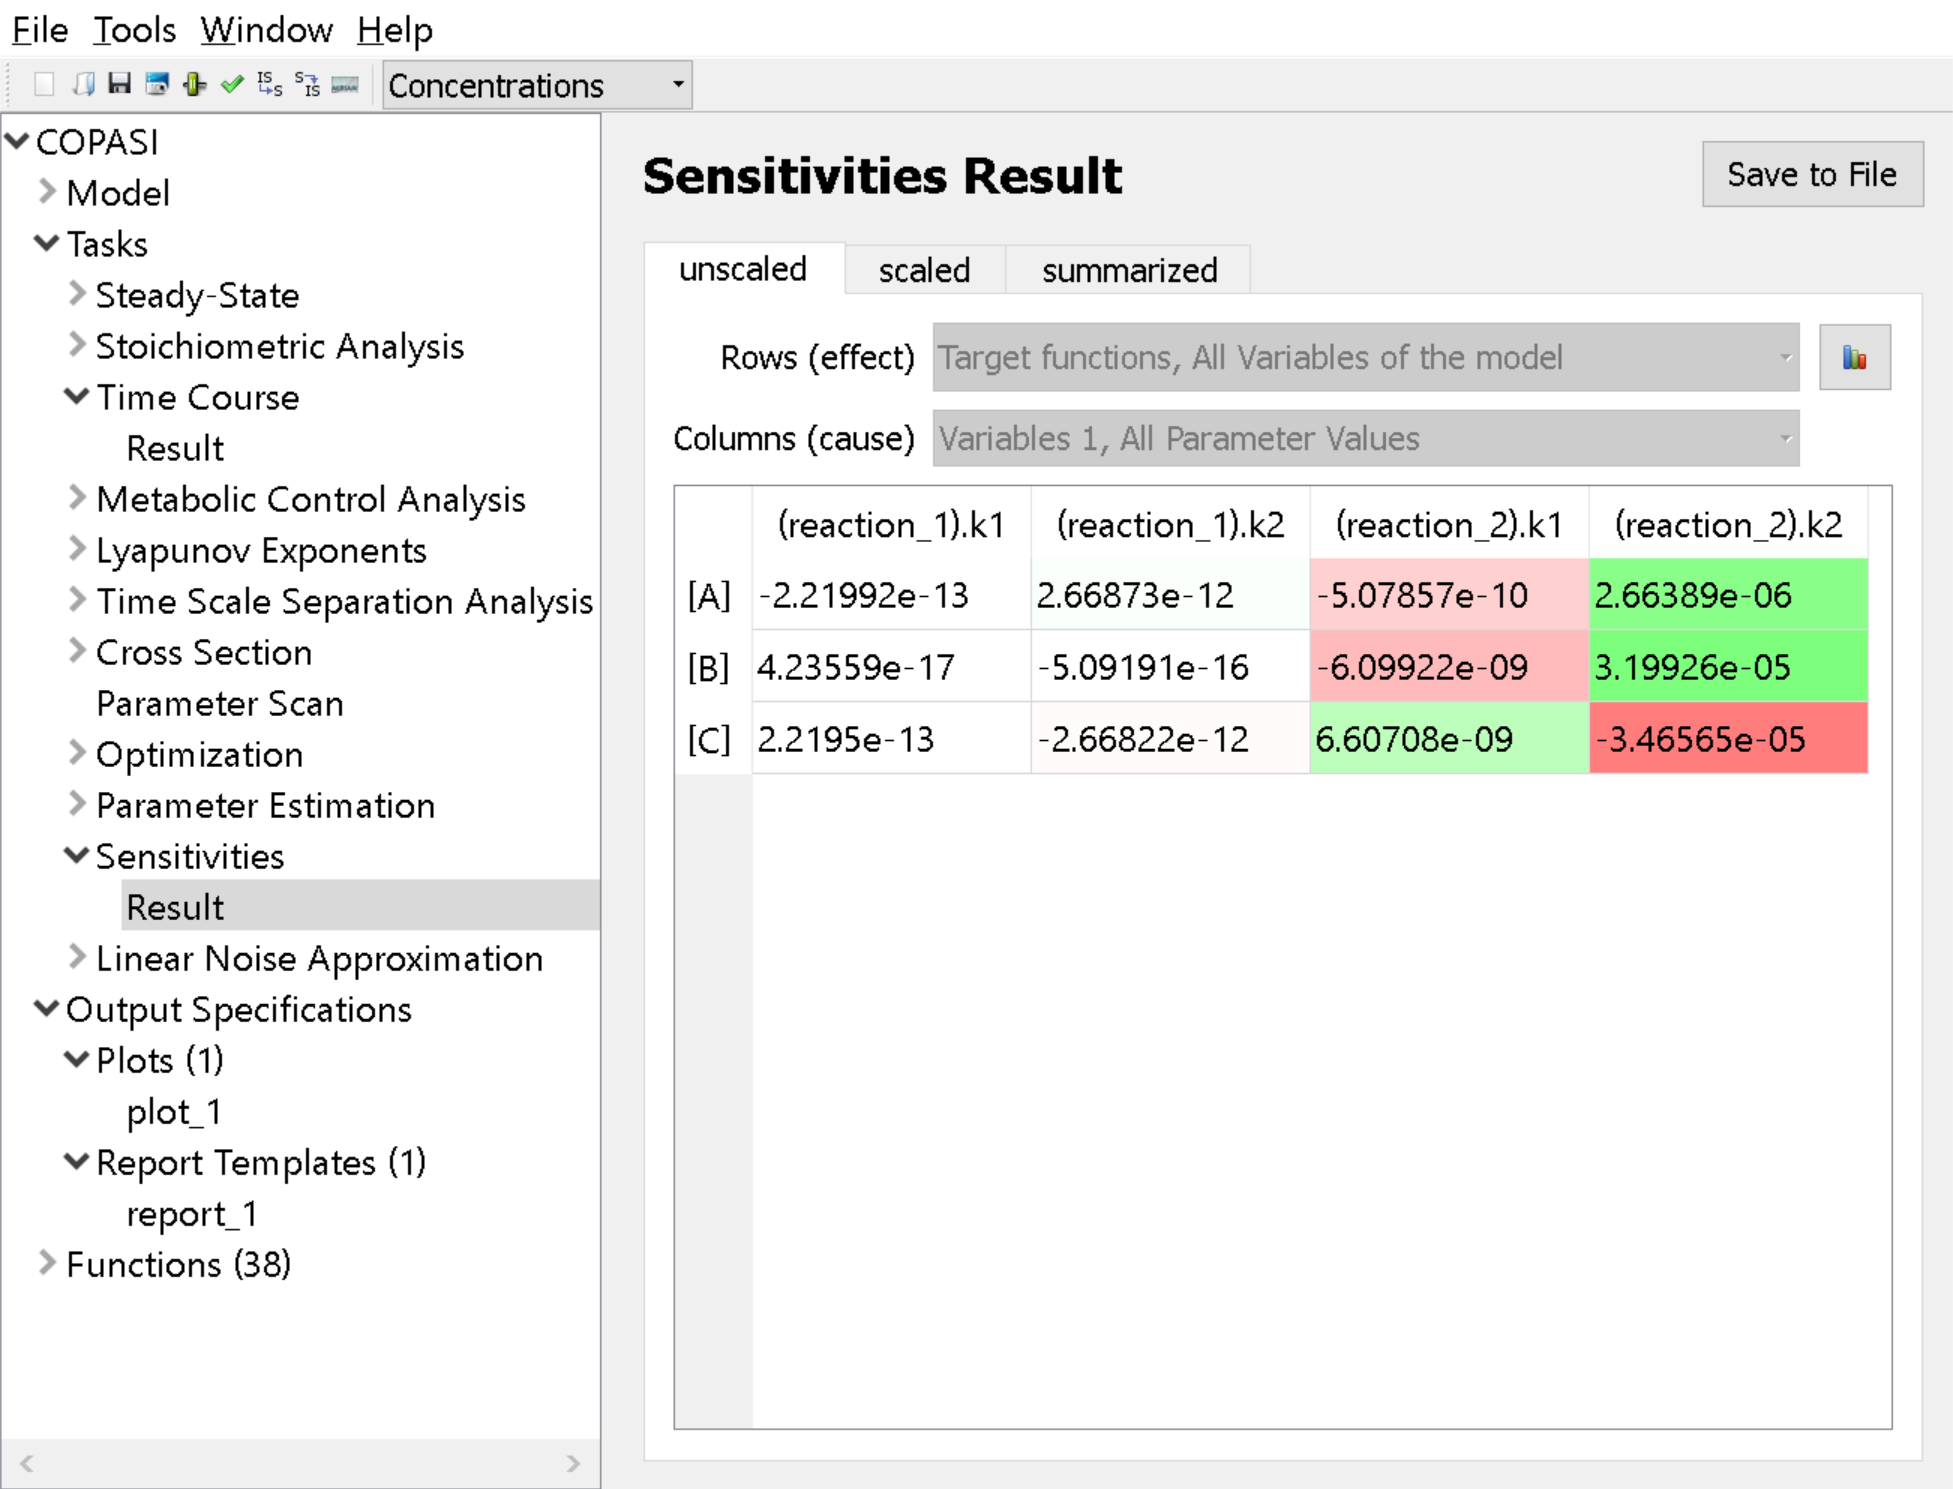
\includegraphics[height=5cm]{Images/11b.png}
		\caption{Sensitivity Analysis}
		\label{11png}
	\end{figure}
	\begin{enumerate}[start=1]\def\makelabel{\textbf{Step}~}
		\item In the \textbf{Object tree}, under \textbf{Tasks}, select \textbf{Sensitivities}.
		\item In the \textbf{Editor} pane, select the  \textbf{Subtask} as \textbf{Steady State} from the drop down menu.
		\item Choose the variables to analyze (\textbf{Effect} as \textbf{All Variables of the model}) with respect to the parameters (\textbf{Cause} as \textbf{All Parameter Values}) . (Leave the \textbf{Secondary Cause} as \textbf{Not Set})
		\item In the \textbf{Editor} pane, select \textbf{Report} from the bottom right and choose a file (\textbf{Sensitivity Report.txt}) to save the report.
		\item Click on Run.
		\item In the \textbf{Object tree}, under \textbf{Sensitivities}, select \textbf{Results}. This will show the \textbf{Scaled} and \textbf{Unscaled} sensitivities calculated.
	\end{enumerate}
	
		
		\section{Parameter Estimation}
		In most of the situation, parameters of the system are unknown. COPASI's parameter estimation is a great tool to identify the unknown parameters. COPASI uses the time-evolution or steady state data to determine the parameters of the system employing a variety of methods. 
		\subsection*{Setup-Figure~\ref{10png}}
		\begin{figure}[!htb]
			\centering
			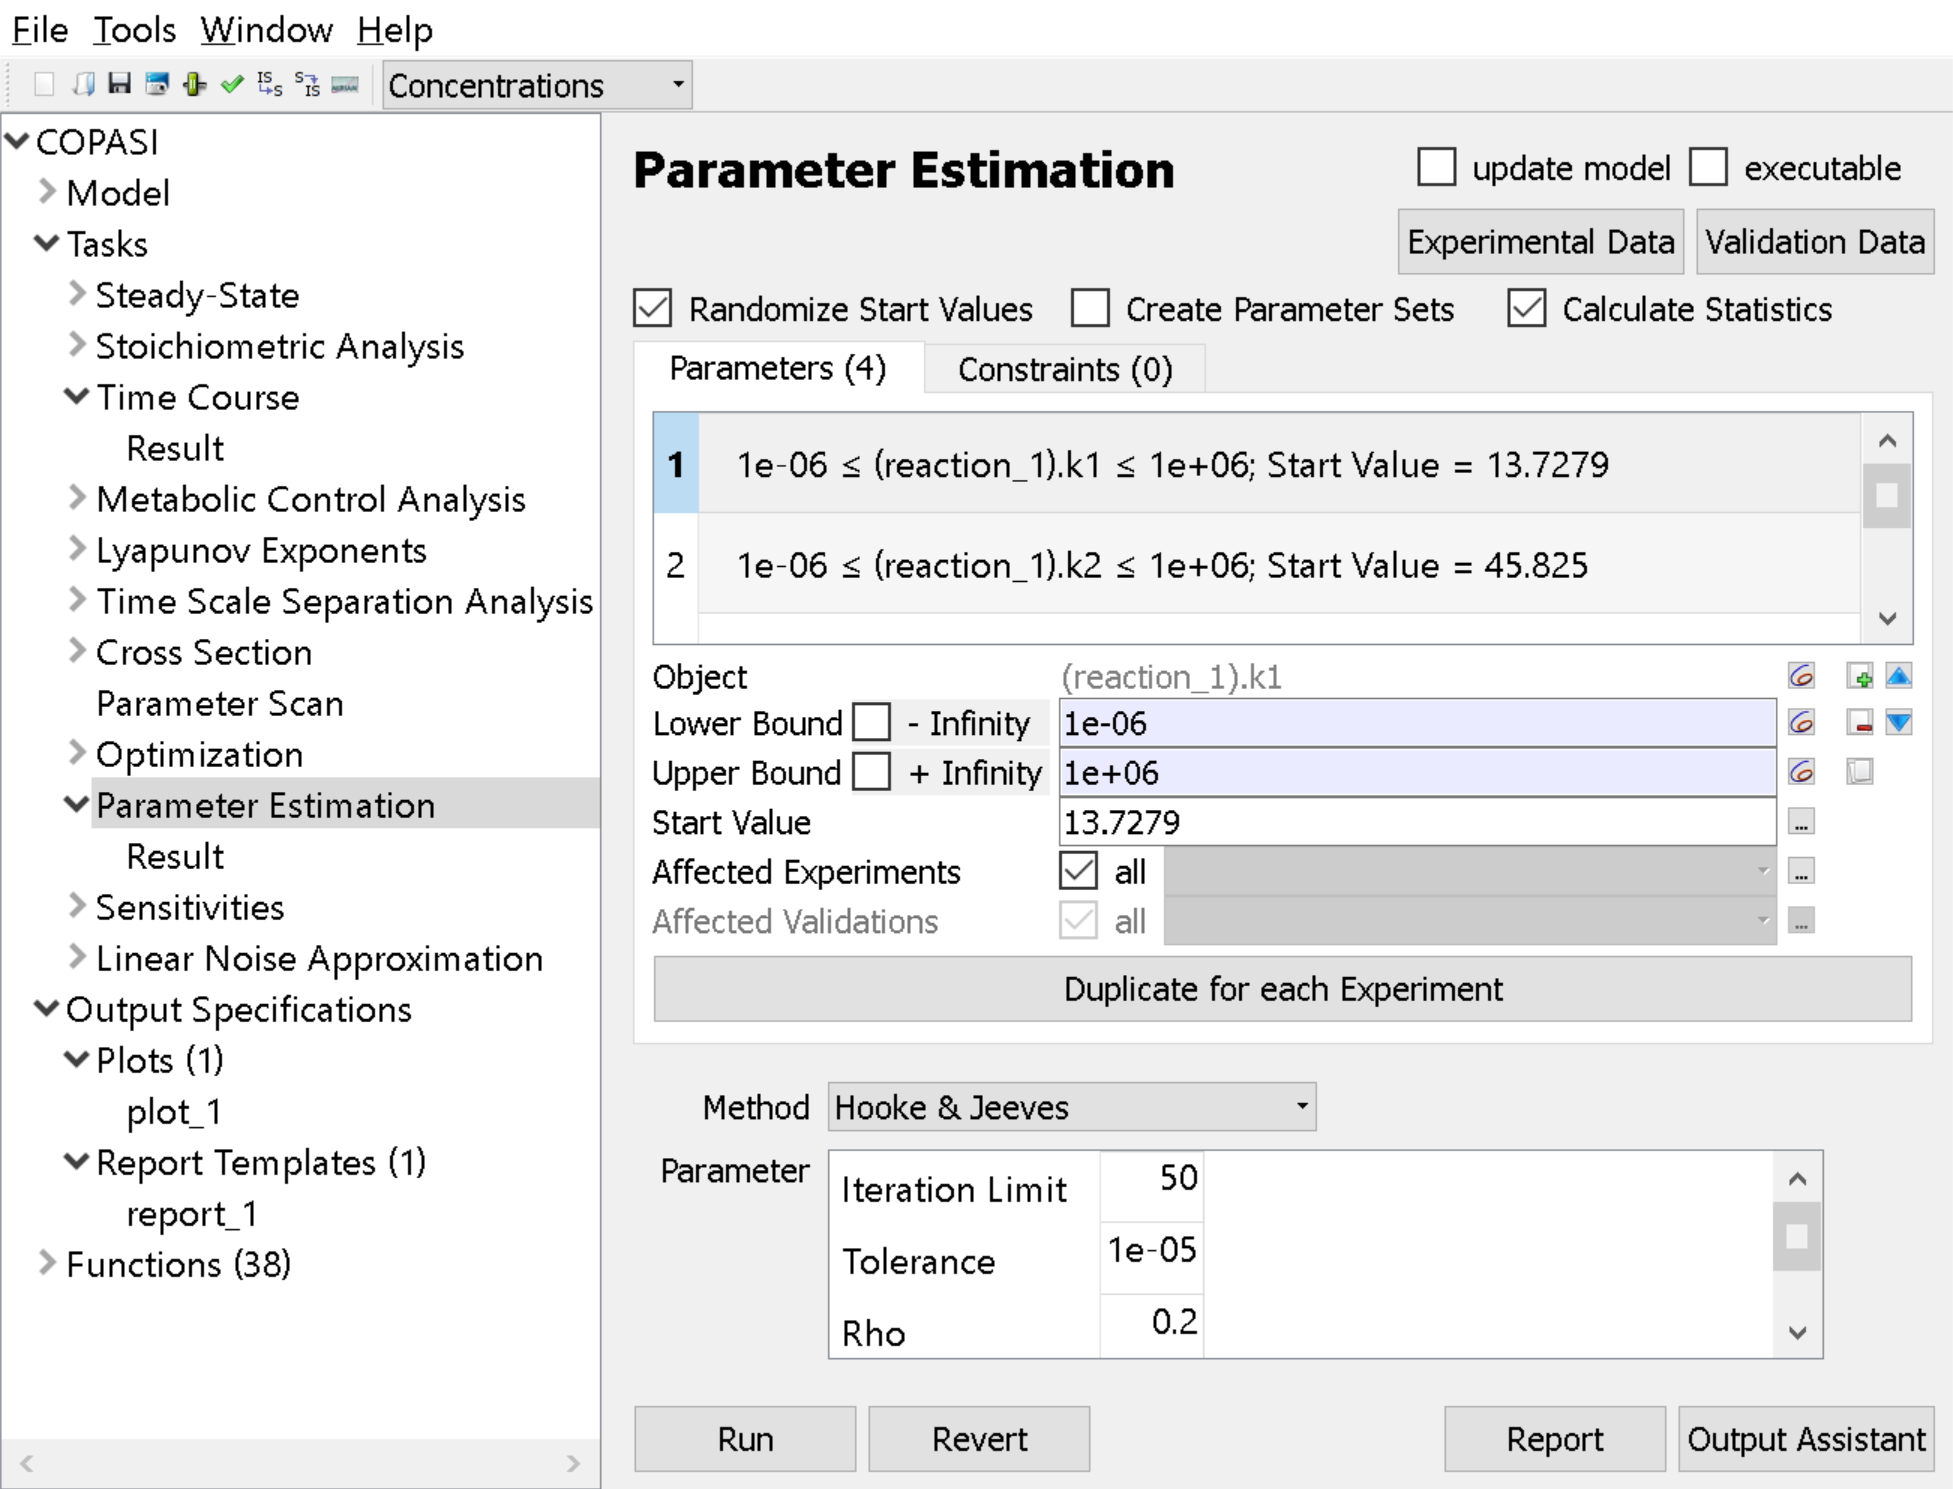
\includegraphics[height=5cm]{Images/10a.png}
			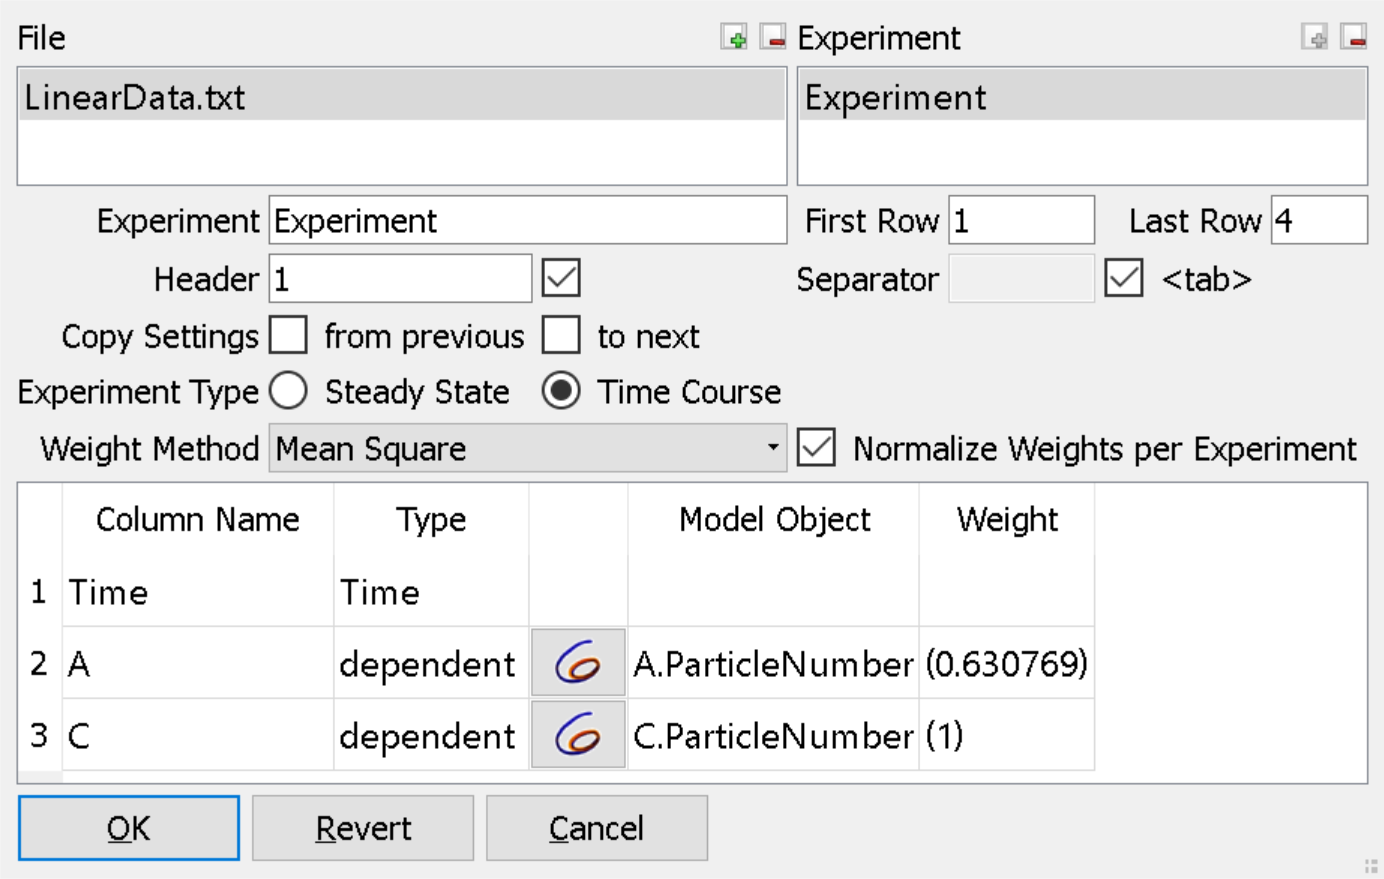
\includegraphics[height=5cm]{Images/10b.png}
			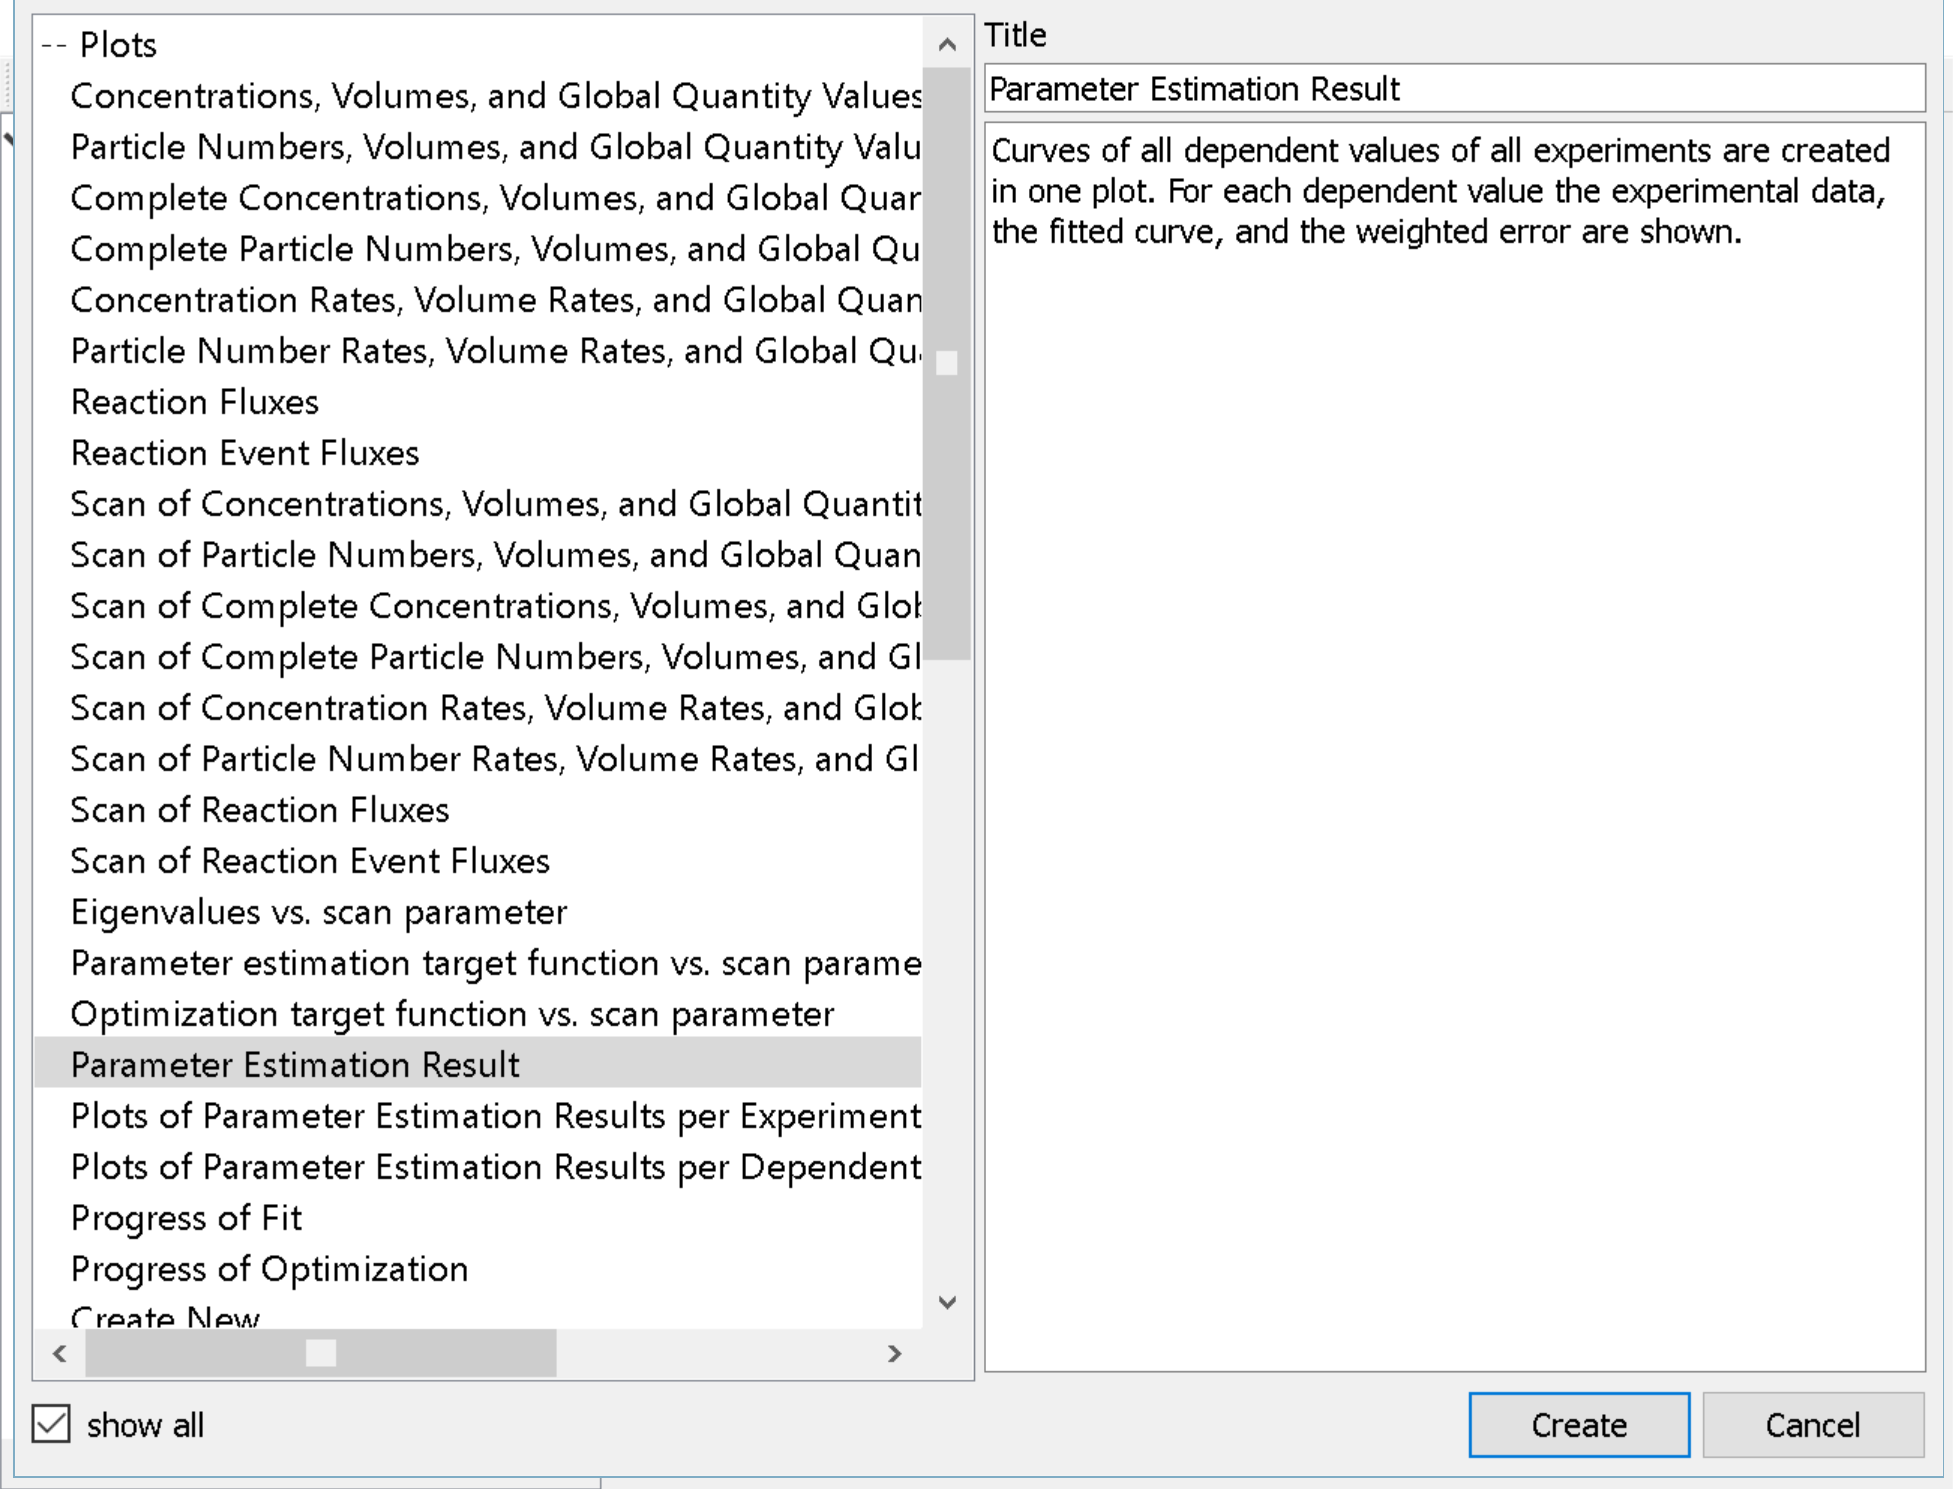
\includegraphics[height=5cm]{Images/10c.png}
			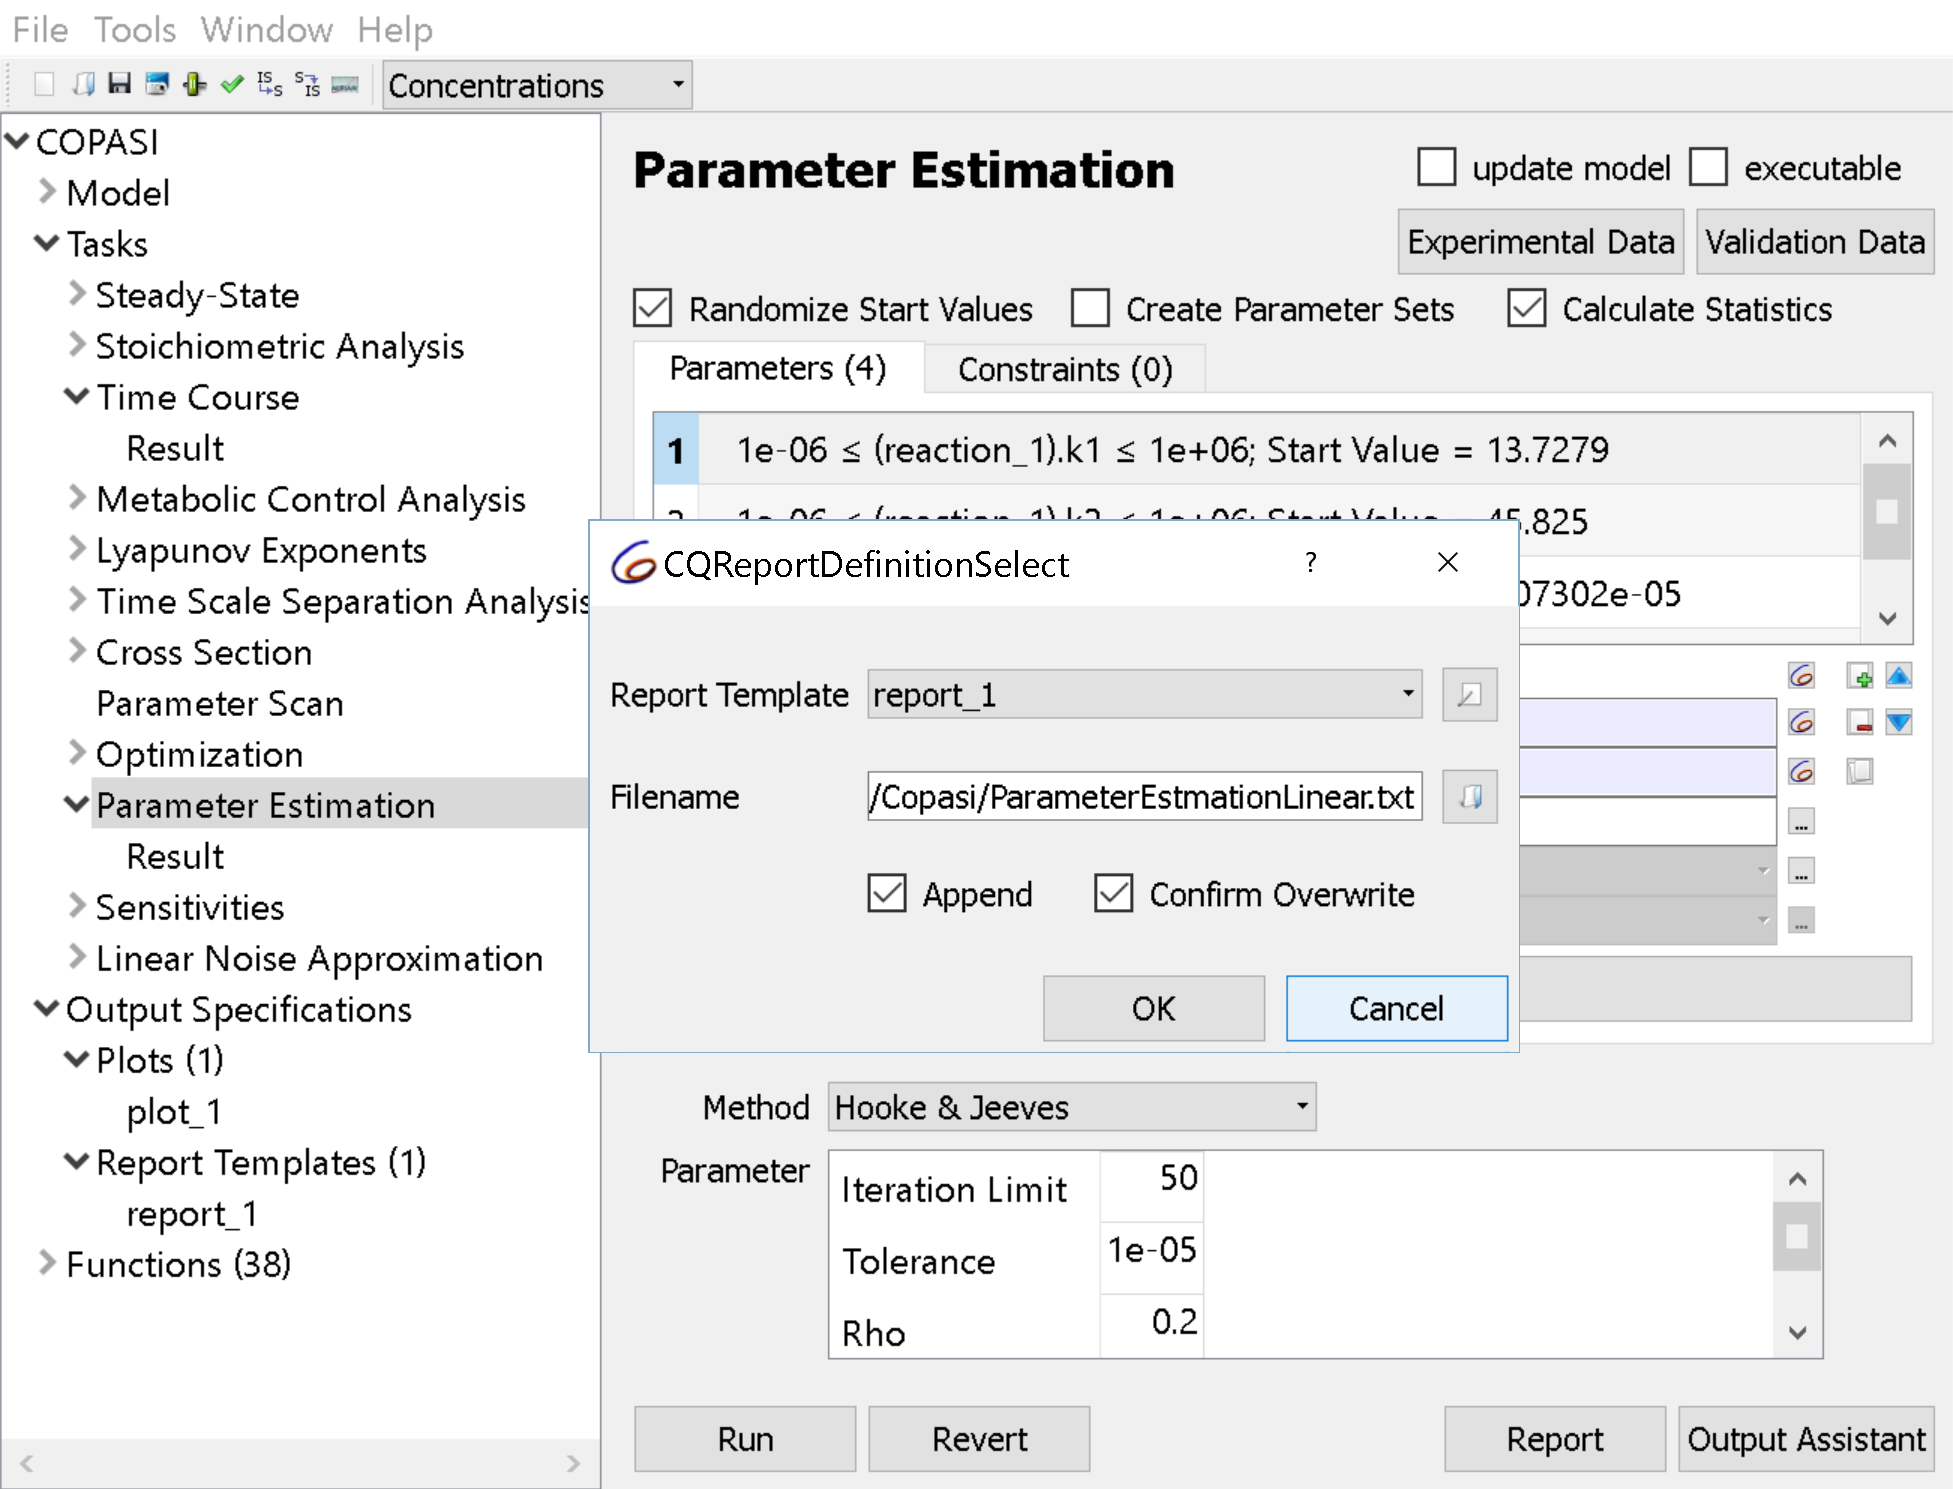
\includegraphics[height=5cm]{Images/10d.png}
			\caption{Parameter Estimation setup}
			\label{10png}
		\end{figure}
		\begin{enumerate}[start=1]\def\makelabel{\textbf{Step}~}
			\item In the \textbf{Object tree}, under \textbf{Tasks}, click on \textbf{Parameter Estimation}
			\item In the \textbf{Editor} pane, click on \textbf{Experimental Data} (for which we need to estimate the parameters of the system). This will open a pop-up window-\textbf{Experimental Data}. 
			\item In the \textbf{Experimental Data} window, we need to import the file that has experimental data. Download the file \textbf{Experimental Data-Timecourse Linear.txt} from dropbox.
			\item In the \textbf{Experimental Data} window, choose the browse button next to \textbf{File} and select the file  \textbf{Experimental Data-Timecourse Linear.txt}.
			\item In \textbf{Experiment Type}, Choose \textbf{Time Course} since our data is a time course result.
			\item In the bottom Data box, under Column \textbf{Type}, choose \textbf{Time} corresponding to \textbf{Time} in the \textbf{Column Name}. For the species \textbf{A} and \textbf{B} in the \textbf{Column Name}, Choose \textbf{Type} as \textbf{dependent} and select the type of data in the experimental data (\textbf{Transient Particle Numbers} \textbf{A(t) \& C(t)}) 
			\item Click \textbf{OK}
			\item In the \textbf{Editor} pane, Choose the the parameters to be identified using \textbf{Object}. Click on the COPASI sign next to \textbf{Object}'s blank cell which will open a pop up window-{Select Items}.
			\begin{enumerate}
				\item Under Reactions, choose \textbf{Reaction Parameters} which will select all rate constants under \textbf{Reaction parameters}. 
				\item Click \textbf{OK}
			\end{enumerate}
			\item In the bottom box, Choose \textbf{Method} as \textbf{Hooke \& Jeeves}.
			\item To generate a parameter plot, Choose \textbf{Output Assistant} from the bottom right which will open a pop-up Window- {Output Assistant}.
			\begin{enumerate}
				\item In the window, \textbf{Output Assistant}, choose a predefined plot \textbf{Parameter Estimation Result} (note: make sure \textbf{show all} check box in the bottom left is checked).
				\item click on \textbf{Create}.        
			\end{enumerate}
			\item In the \textbf{Editor} pane, click on \textbf{Run}. This will identify optimal parameter values, generates a time course plot predicted with determined parameters, error with the experimental data, and a detailed report of the parameter estimation.
		\end{enumerate}
		\subsection*{Results-Figure~\ref{Result2}}
		\begin{figure}[!htb]
			\centering
			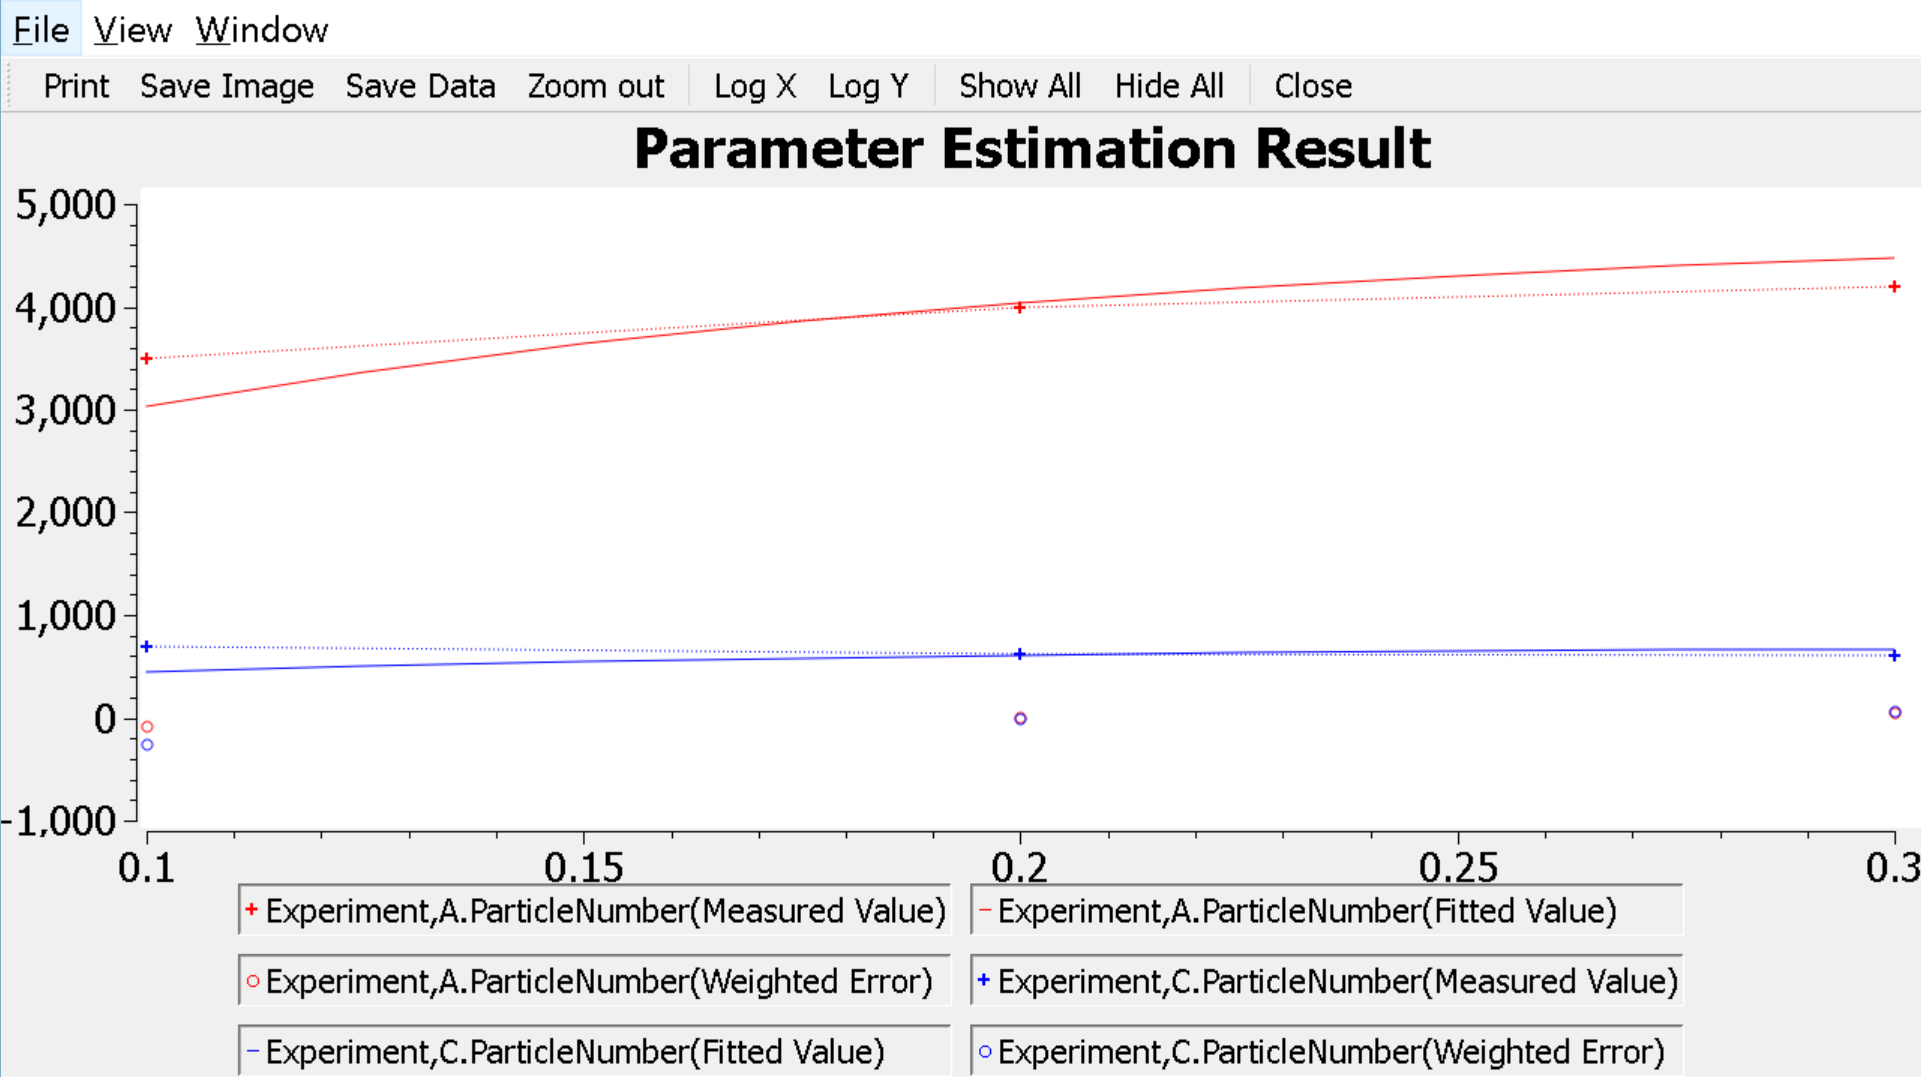
\includegraphics[height=5cm]{Images/R2a.png}
			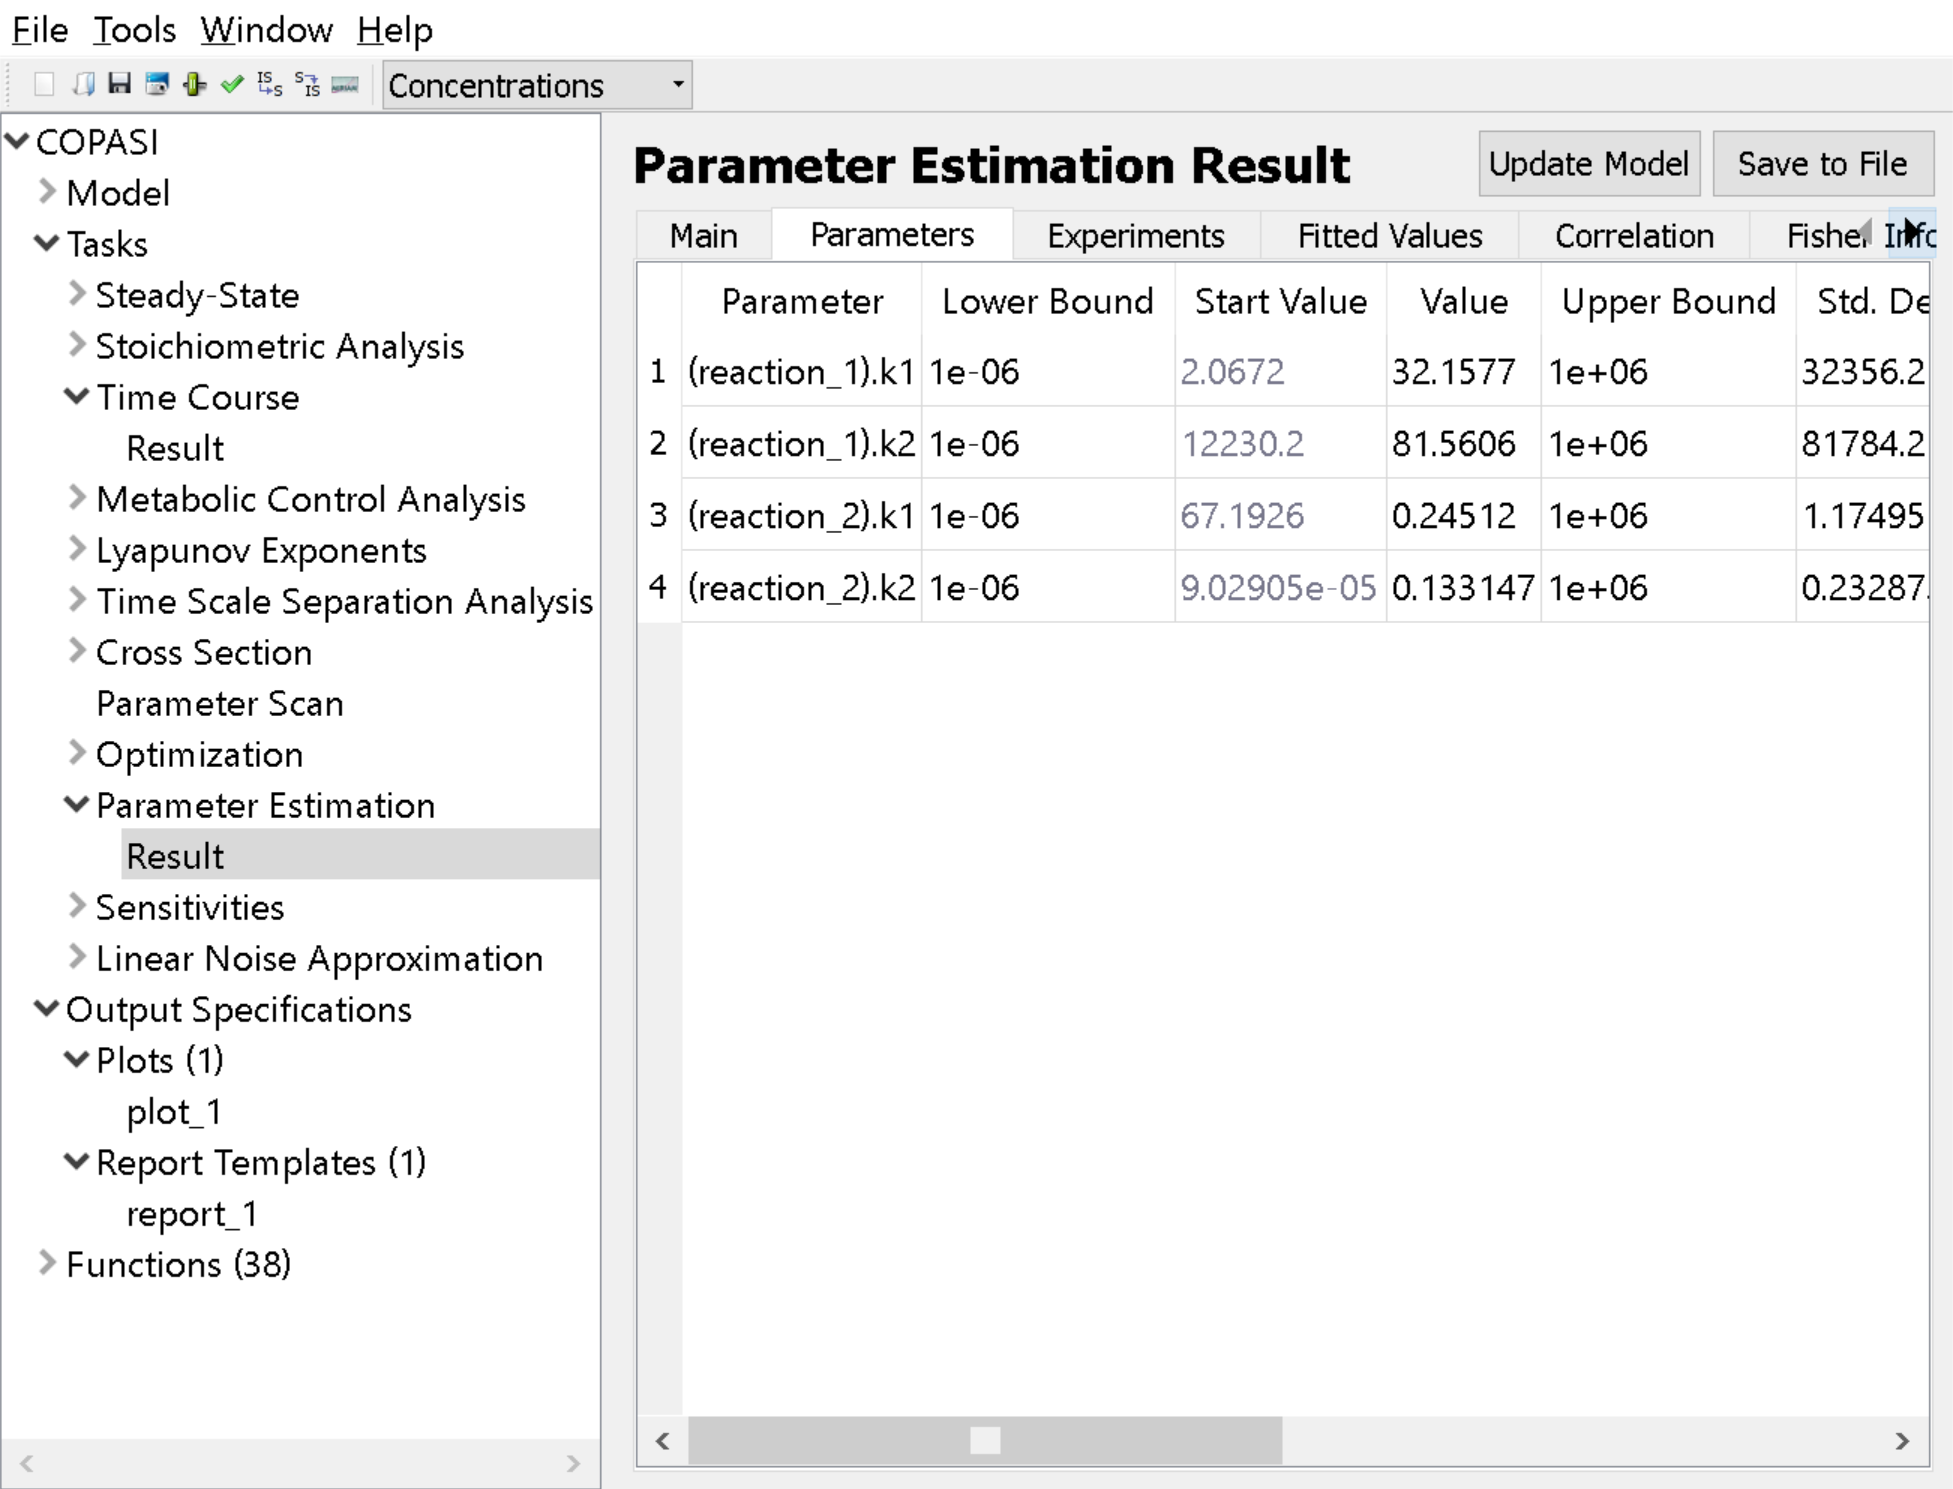
\includegraphics[height=8cm]{Images/R2b.png}
			\caption{Parameter Estimation Results}
			\label{Result2}
		\end{figure}
		\begin{enumerate}[start=1]\def\makelabel{\textbf{Step}~}
			\item In the \textbf{Object tree}, under \textbf{Parameter Estimation}, select \textbf{Results}
			\item In the \textbf{Editor} pane, choose \textbf{Parameters} tab. Under \textbf{Values}, we can see the optimal values identified. 
			\item We can then update the model with these parameters using \textbf{Update Model} located at the top right of \textbf{Editor} pane. If we run the time course analysis again, we can compare the experimental data with the simulated results.
		\end{enumerate}				
	
	\section{Exercise: Gene regulatory Networks}
	\subsection*{Autoinhibition}
	\begin{enumerate}
		\item Download the model of an auto inhibitory gene (\textbf{GRN-AutoInhibition.cps}) from the Dropbox.
		
		\item Determine the sensitivity of the steady state protein concentration (\textbf{P}) to the maximal expression rate ({$\textbf{E}_{\textbf{max}}$}).
		
		\item Reduce the inhibition strength (increase dissociation constant $\textbf{K}$) and confirm that the sensitivity of the unregulated protein level is higher.
		
		\item If you increase the inhibition strength (decrease dissociation constant $\textbf{K}$) you can reduce the sensitivity significantly. What would be the downside of very strong inhibition?
		
		\item Modify the model so that the protein product *activates* expression. Confirm that the sensitivity to the maximum expression rate is high in this case. 

		\item Introduce cooperativity to the activation term, and confirm that the system can act as a bistable switch.
	\end{enumerate}
	
\subsection*{Goodwin Oscillator}
	\begin{enumerate}
		\item Open Goodwin oscillator model (\textbf{Goodwin Oscillator.cps}) from the dropbox.
		\item Modify the model by adding a fourth step to the activation cascade. (Use dynamics identical to the third step.) Verify that the additional lag introduced by this fourth component allows the system to exhibit sustained oscillations with n < 8.
		\item Replace the term for degradation of Z by a Michaelis-Menten term: $\delta Z/(K_M + Z)$. Verify that this modified system oscillates with no cooperativity (i.e. with n = 1). Take $a = 150\ concentration. time^{-1}, k = 1\ concentration,b = \alpha = \beta = \gamma= 0.2\  time^{-1}$ , $\delta = 15\ time^{-1}$, and $K_M = 1$.
	\end{enumerate}
	
	\section*{Additional Tasks}
	\subsection*{Steady State-Figure~\ref{12png}}
	\begin{figure}[!htb]
		\centering
		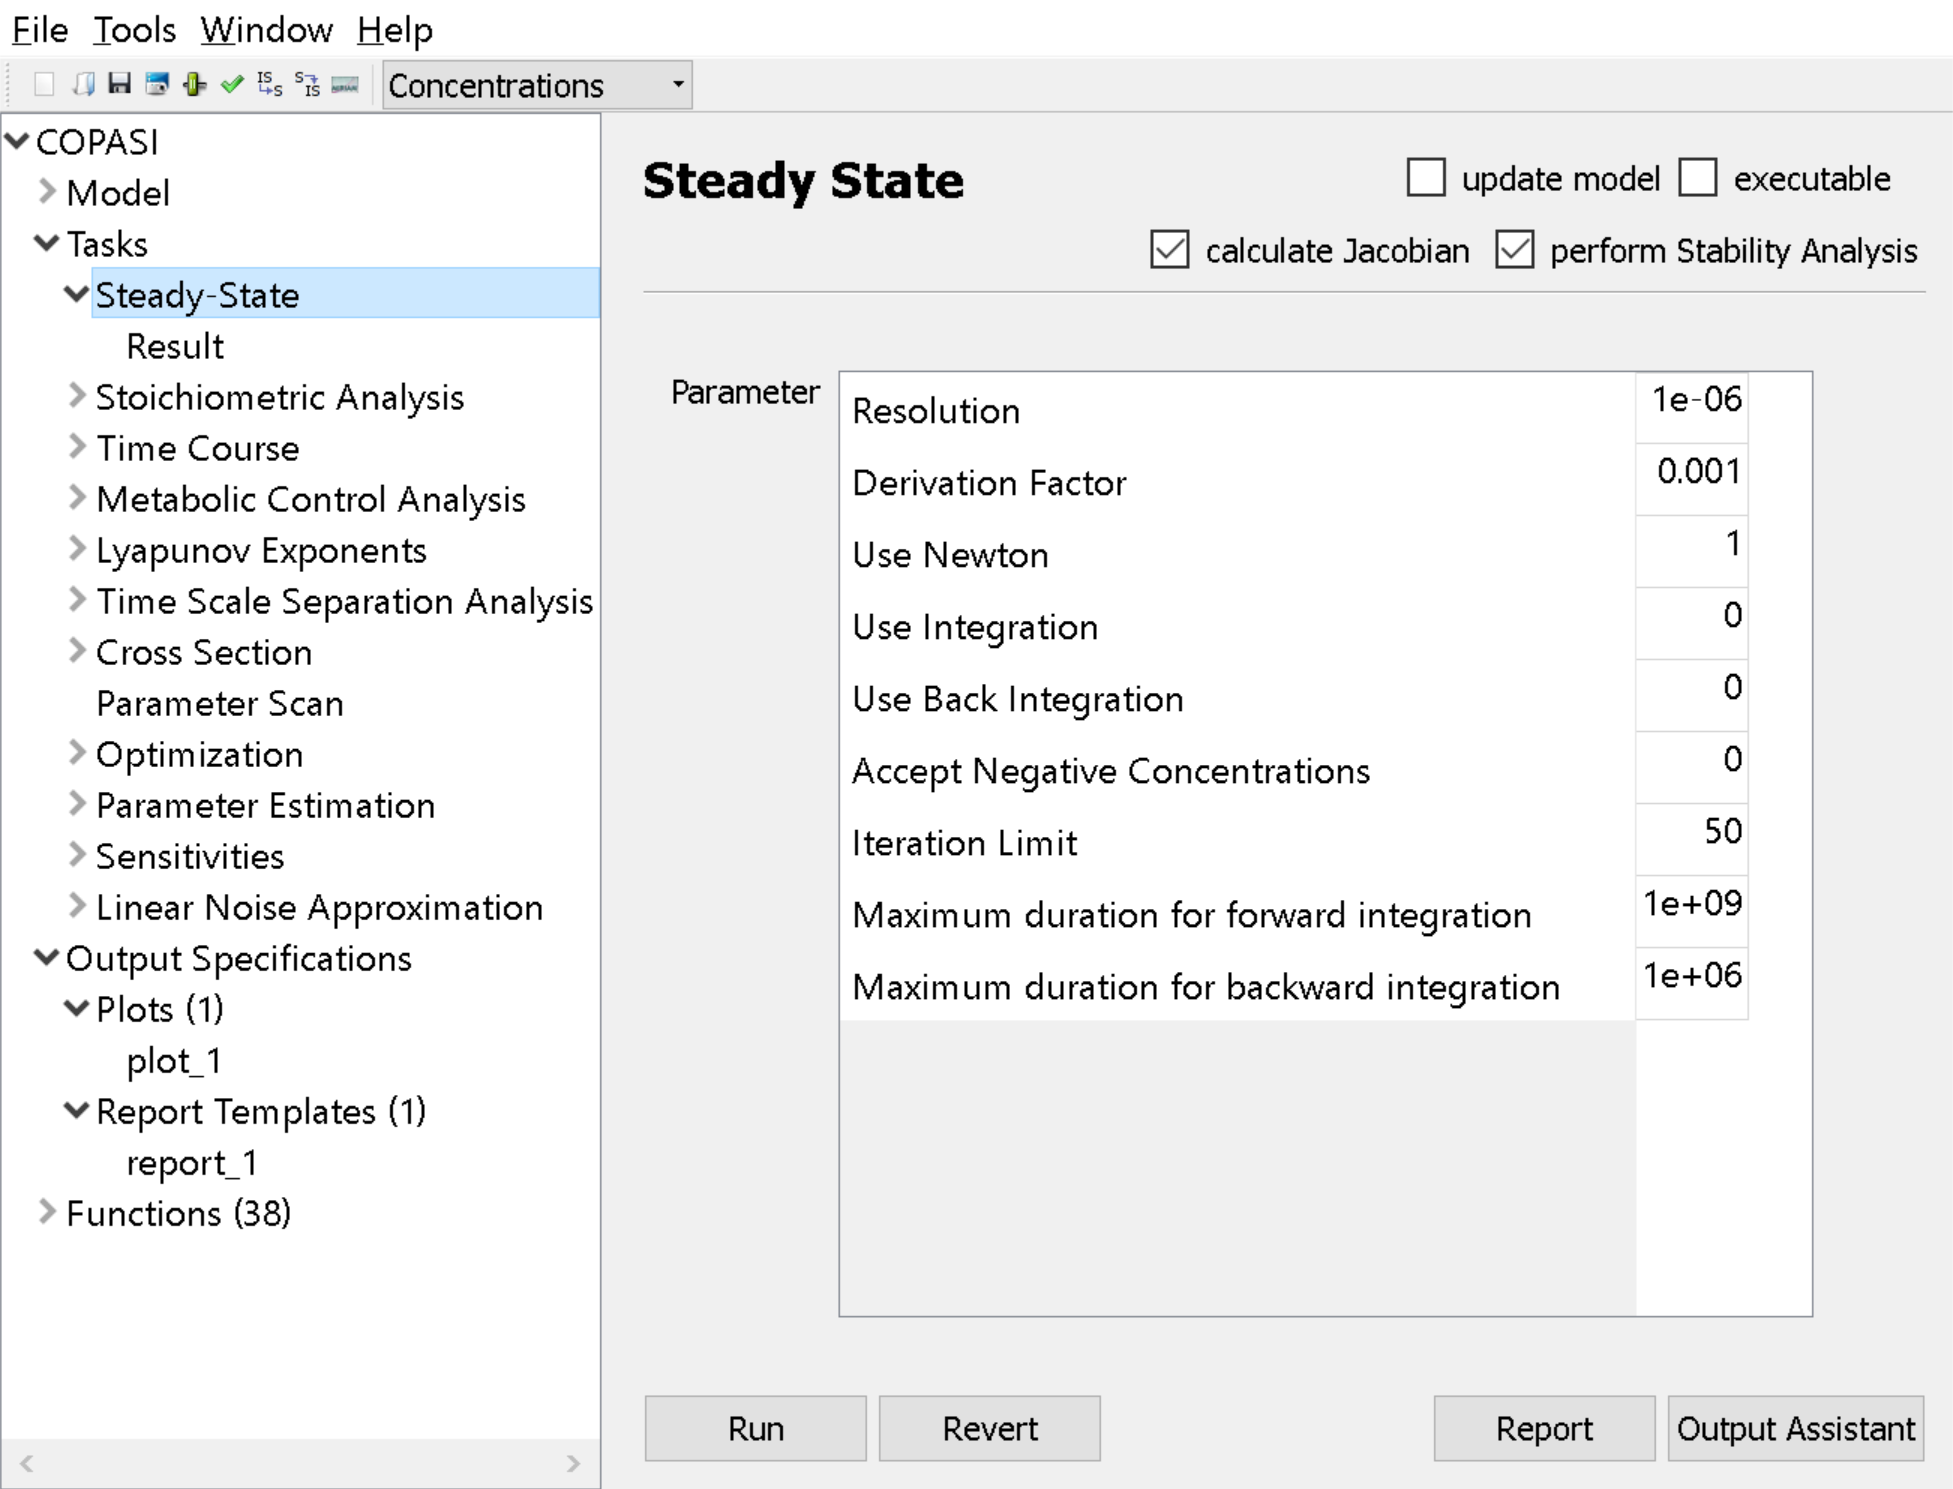
\includegraphics[height=5cm]{Images/12a.png}
		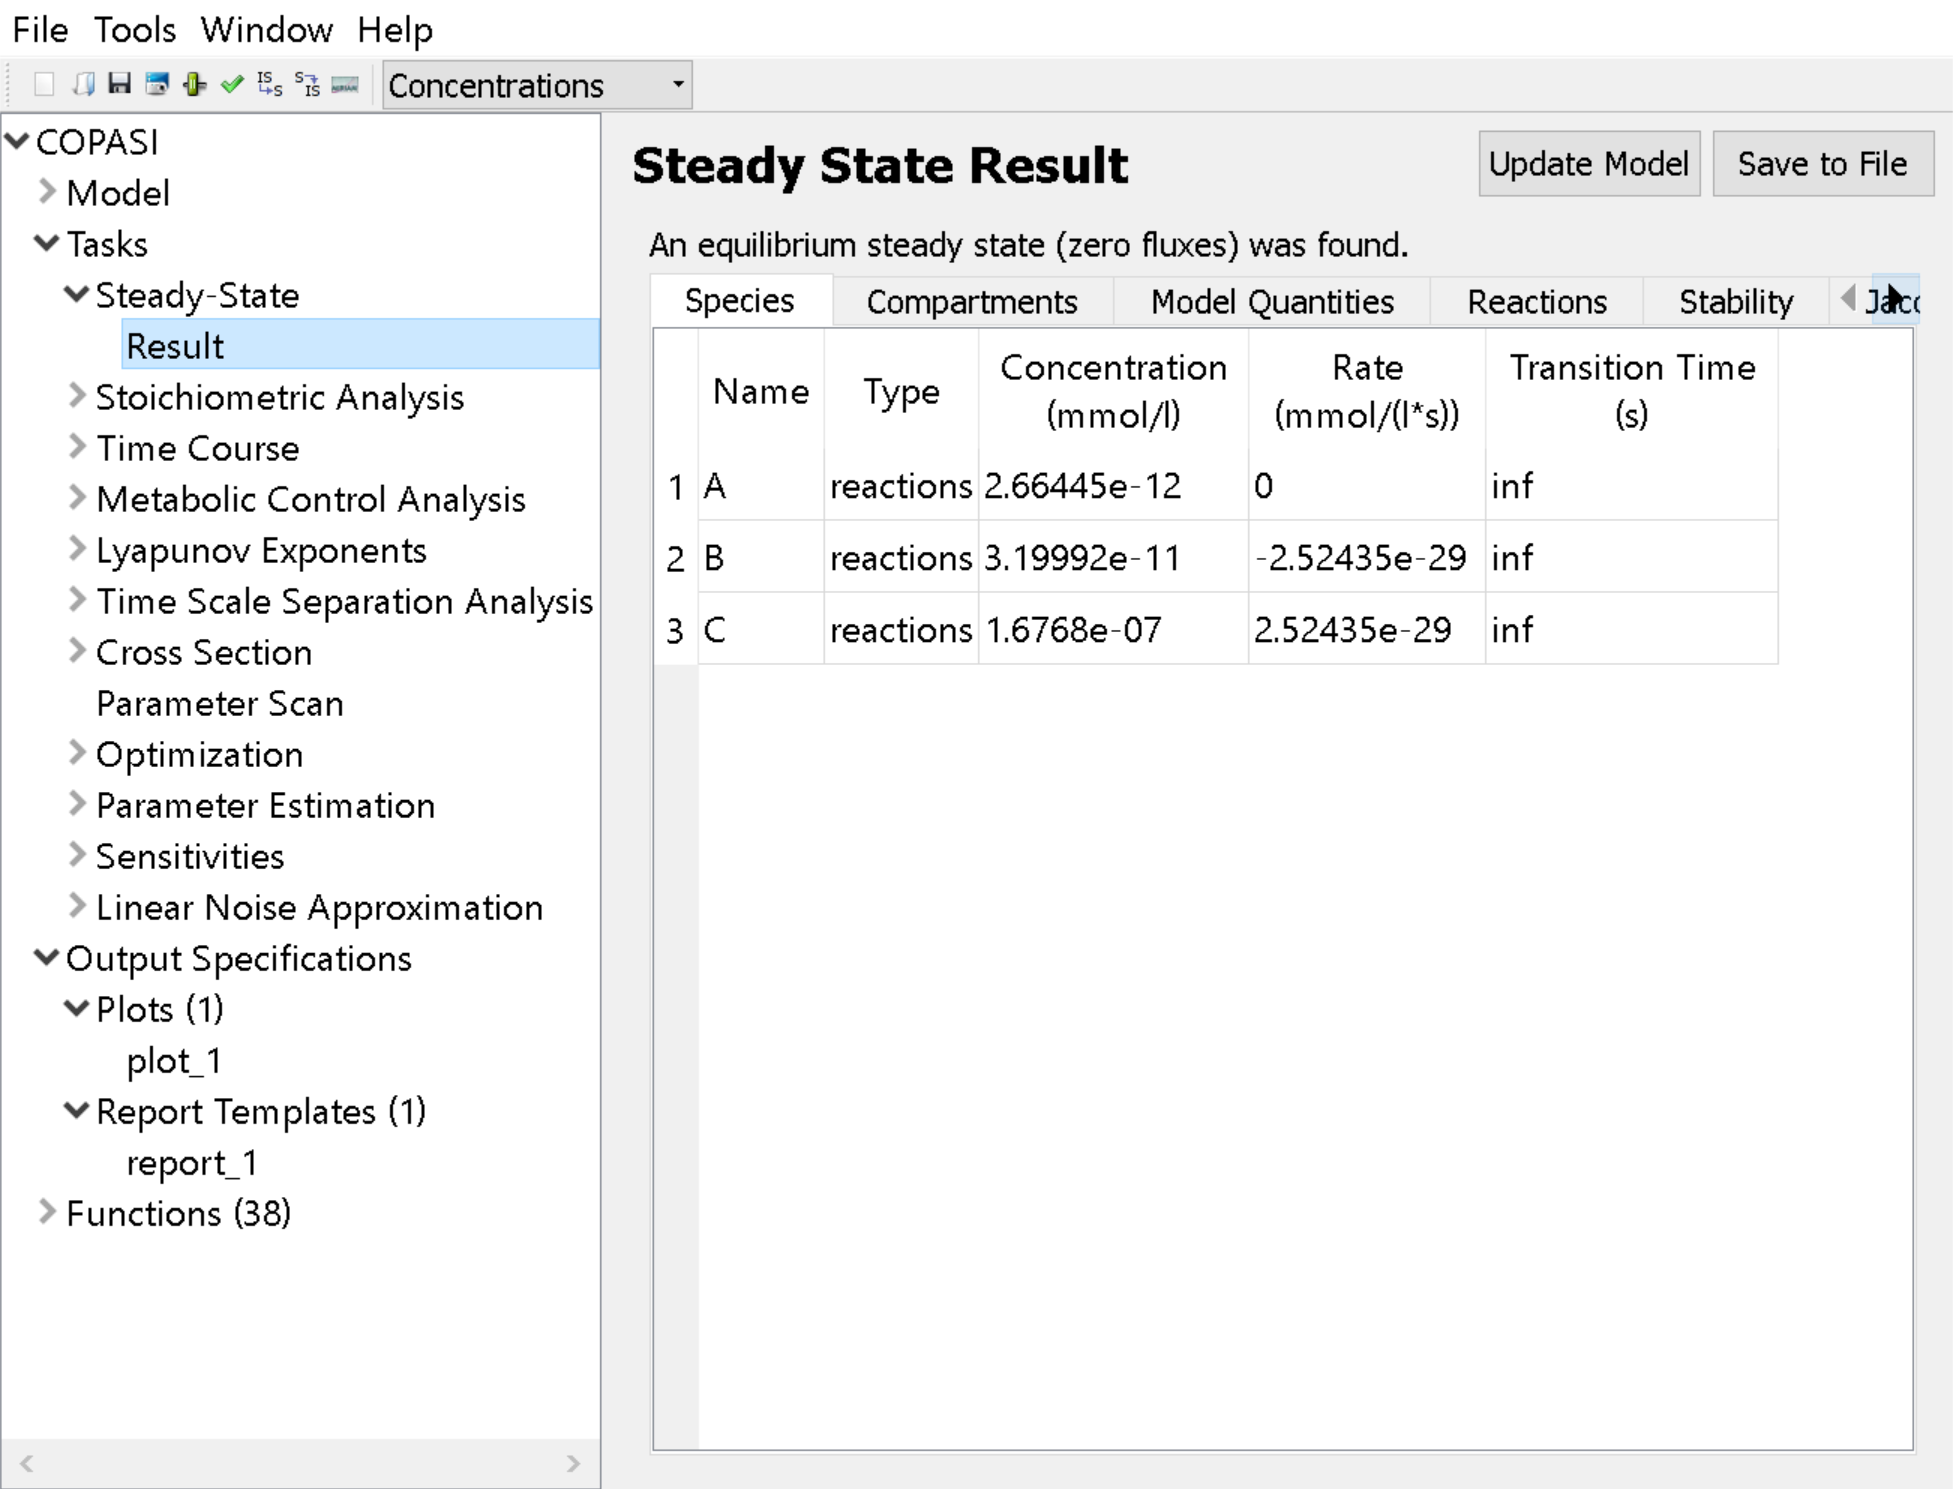
\includegraphics[height=5cm]{Images/12b.png}
		\caption{Steady state}
		\label{12png}
	\end{figure}
	
	In steady state analysis, we will be identifying steady state concentration of each species and the stability of the steady state. There are three methods to identify the steady state. They are \textbf{Newton's method}, \textbf{Integration} and \textbf{Back Integration}. 
	\begin{enumerate}[start=1]\def\makelabel{\textbf{Step}~}
		\item In the \textbf{Object tree}, under \textbf{Tasks}, select \textbf{Steady-State}
		\item In the \textbf{Editor} pane, Check \textbf{Calculate Jacobian} and \textbf{perform Stability Analysis} for computing the stability
		\item Enter \textbf{1} in the cell corresponds to \textbf{Use Newton} and keep other two methods value to \textbf{zero}. (Note:choose the method using a boolean value (\textbf{0} or \textbf{1}).
		\item (optional) Choose the number of iteration in Newton's method by choosing \textbf{Iteration Limit}
		\item Click on \textbf{Run}
		\item In the \textbf{Object tree}, choose \textbf{Results} under \textbf{Steady-State}.
		\item In the \textbf{Editor} pane, choose the tab \textbf{Species}. Here we can see the steady state concentration of each species under column \textbf{Concentration}. Note that the column \textbf{Rate} has values close to zero (less than $10^{-12}$). If it is not close to zero, then the steady state is not identified using Newton's method with given accuracy. This will be mentioned at one row above \textbf{Species} tab. Then to find the steady state, either change values of \textbf{Resolution}, \textbf{Derivative Factor}, and/or \textbf{Iteration Limit}) or change the methods to \textbf{Integration} or \textbf{Back Integration} methods.
		\item Once we found the steady state, select \textbf{Stability} tab in the \textbf{Editor} pane. Here we can see the summary of stability of steady state.
	\end{enumerate}
	
	\subsection*{Stoichiometry Analysis-Figure~\ref{13png}}
	\begin{figure}[!htb]
		\centering
		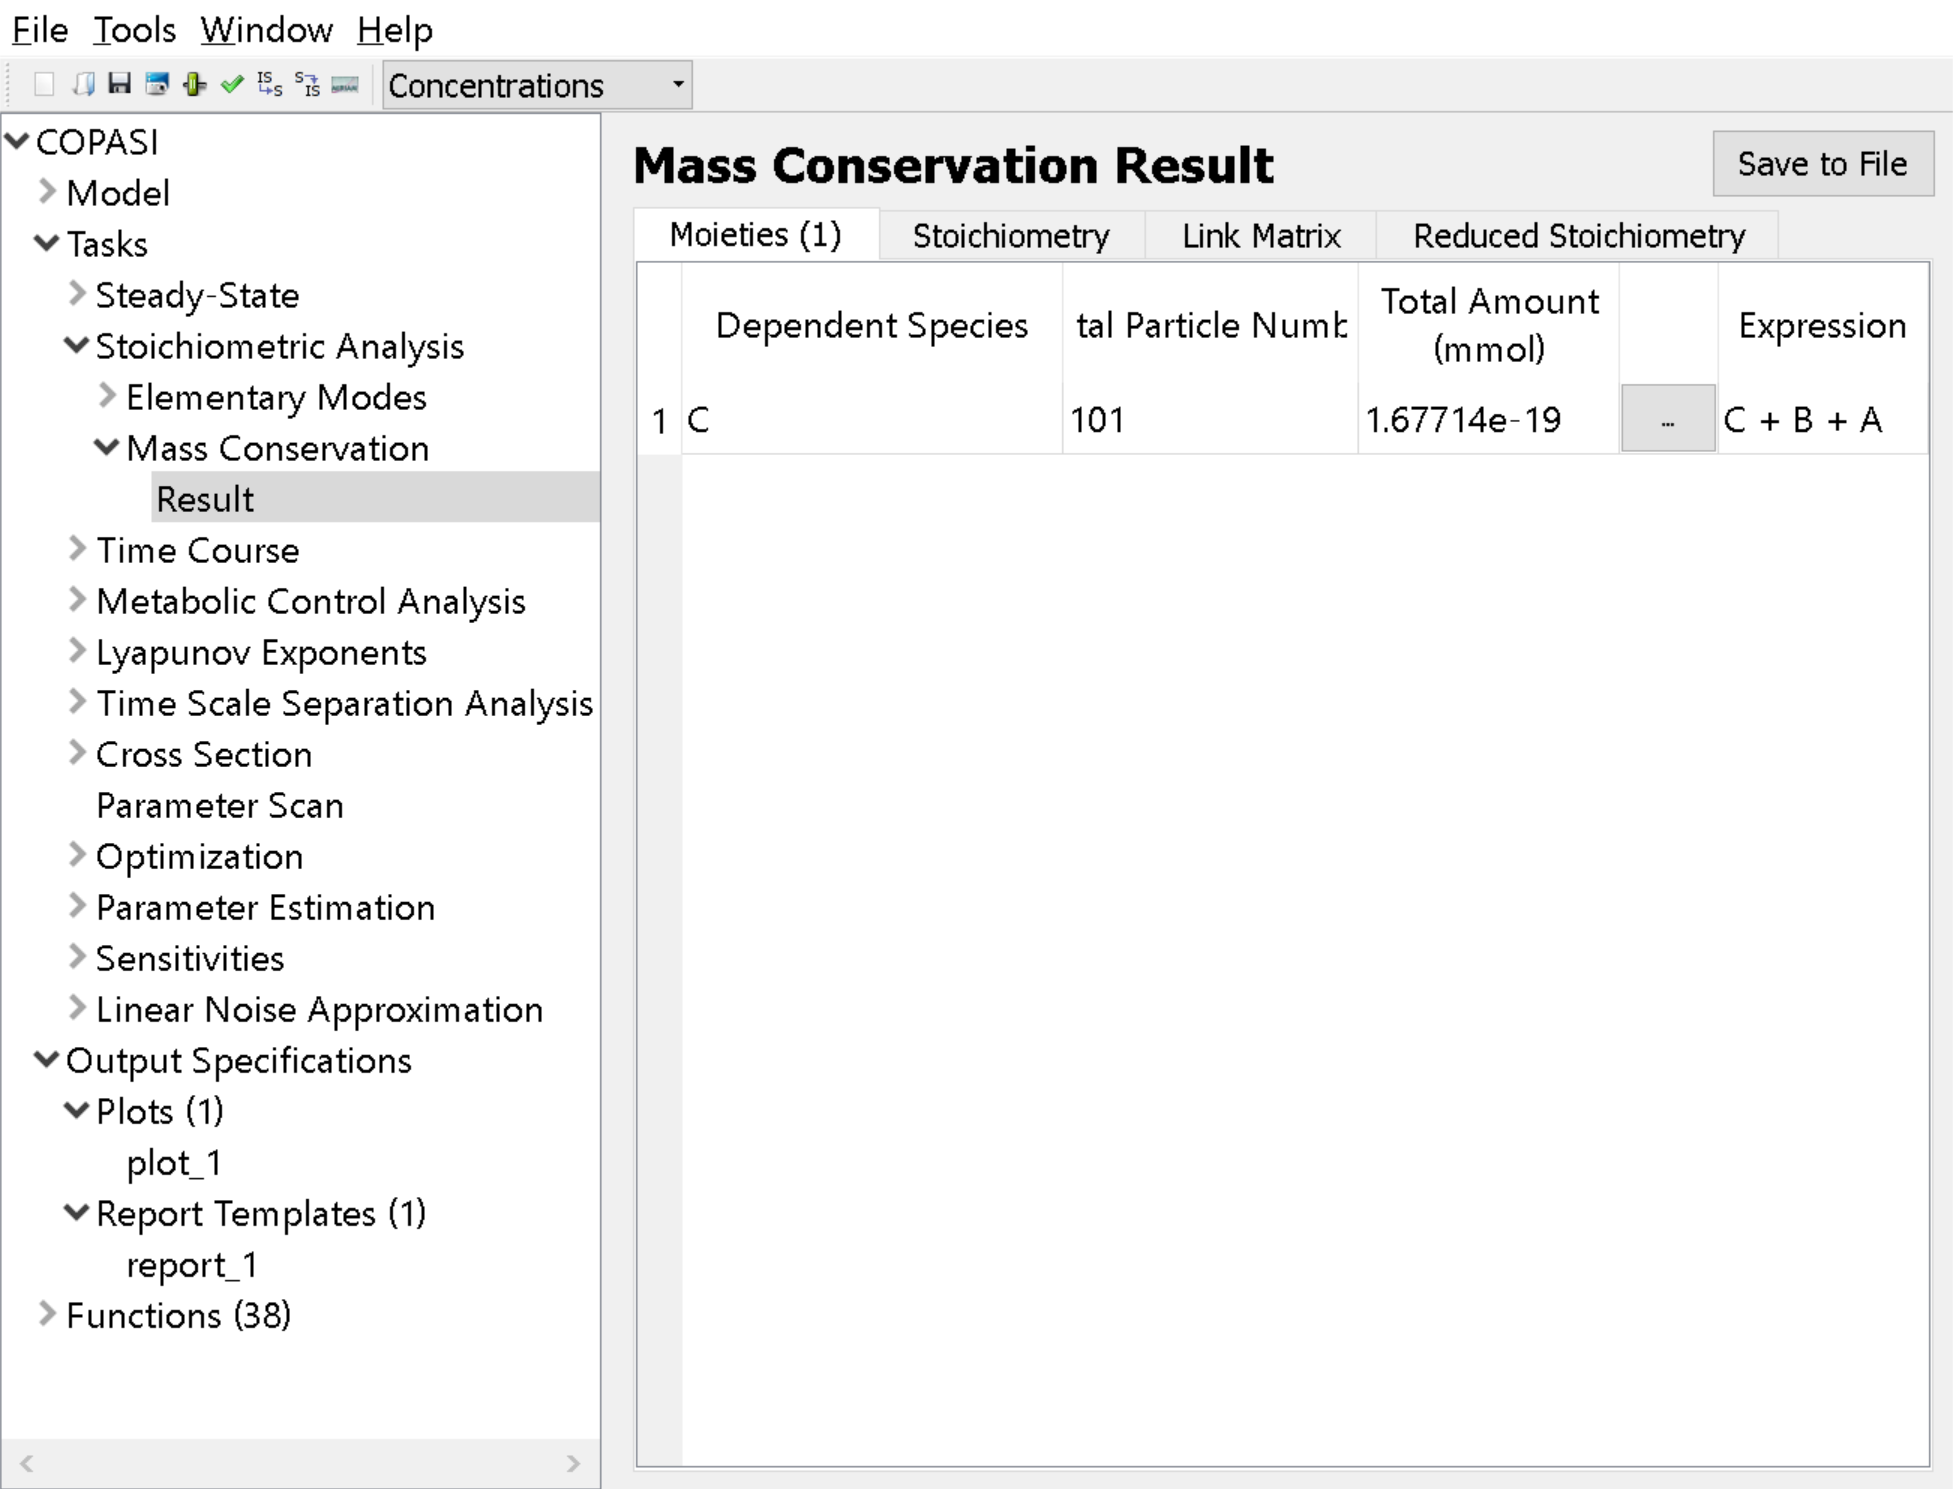
\includegraphics[height=5cm]{Images/13a.png}
		\caption{Stoichiometry Analysis}
		\label{13png}
	\end{figure}
	In stoichiometry analysis, we identify the mass conservation laws available in the system.
	\begin{enumerate}[start=1]\def\makelabel{\textbf{Step}~}
		\item In the \textbf{Object tree}, under \textbf{Tasks}, expand \textbf{Stoichiometry Analysis} and select \textbf{Mass Conservation}.
		\item In the \textbf{Editor} pane, Click on \textbf{Run} and \textbf{Results} will be shown in the \textbf{Editor} pane.
		\item Under the \textbf{Moieties} tab, we can see a number of mass conservations (A+B+C=constant for all time) available in the system.
	\end{enumerate}
	
	
	
	
	
	
	
	
	
\end{document}